
% AGUJournalTemplate.tex: this template file is for articles formatted with LaTeX
%
% This file includes commands and instructions
% given in the order necessary to produce a final output that will
% satisfy AGU requirements, including customized APA reference formatting.
%
% You may copy this file and give it your
% article name, and enter your text.
%
%
% Step 1: Set the \documentclass
%
%

%% To submit your paper:
\documentclass[draft]{agujournal2019}
\usepackage{url} %this package should fix any errors with URLs in refs.
\usepackage{lineno}
\usepackage[inline]{trackchanges} %for better track changes. finalnew option will compile document with changes incorporated.
\usepackage{soul}
\linenumbers

%%%%%%%
% As of 2018 we recommend use of the TrackChanges package to mark revisions.
% The trackchanges package adds five new LaTeX commands:
%
%  \note[editor]{The note}
%  \annote[editor]{Text to annotate}{The note}
%  \add[editor]{Text to add}
%  \remove[editor]{Text to remove}
%  \change[editor]{Text to remove}{Text to add}
%
% complete documentation is here: http://trackchanges.sourceforge.net/
%%%%%%%

\draftfalse

%% Enter journal name below.
%% Choose from this list of Journals:
%
% JGR: Atmospheres
% JGR: Biogeosciences
% JGR: Earth Surface
% JGR: Oceans
% JGR: Planets
% JGR: Solid Earth
% JGR: Space Physics
% Global Biogeochemical Cycles
% Geophysical Research Letters
% Paleoceanography and Paleoclimatology
% Radio Science
% Reviews of Geophysics
% Tectonics
% Space Weather
% Water Resources Research
% Geochemistry, Geophysics, Geosystems
% Journal of Advances in Modeling Earth Systems (JAMES)
% Earth's Future
% Earth and Space Science
% Geohealth
%
% ie, \journalname{Water Resources Research}

\journalname{Journal of Advances in Modeling Earth Systems (JAMES)}


\begin{document}

%% ------------------------------------------------------------------------ %%
%  Title
%
% (A title should be specific, informative, and brief. Use
% abbreviations only if they are defined in the abstract. Titles that
% start with general keywords then specific terms are optimized in
% searches)
%
%% ------------------------------------------------------------------------ %%

% Example: \title{This is a test title}

\title{Impact of grids and dynamical cores in CESM2.2 on the surface mass balance of the Greenland Ice Sheet}

%% ------------------------------------------------------------------------ %%
%
%  AUTHORS AND AFFILIATIONS
%
%% ------------------------------------------------------------------------ %%

% Authors are individuals who have significantly contributed to the
% research and preparation of the article. Group authors are allowed, if
% each author in the group is separately identified in an appendix.)

% List authors by first name or initial followed by last name and
% separated by commas. Use \affil{} to number affiliations, and
% \thanks{} for author notes.
% Additional author notes should be indicated with \thanks{} (for
% example, for current addresses).

% Example: \authors{A. B. Author\affil{1}\thanks{Current address, Antartica}, B. C. Author\affil{2,3}, and D. E.
% Author\affil{3,4}\thanks{Also funded by Monsanto.}}
\authors{Adam R. Herrington\affil{1}, Peter H. Lauritzen\affil{1}, Marcus Lofverstrom\affil{2}, William H. Lipscomb\affil{1}, Andrew Gettelman\affil{1} \ and Mark A. Taylor\affil{3}}

 \affiliation{1}{National Center for Atmospheric Research, 1850 Table Mesa Drive, Boulder, Colorado, USA}
\affiliation{2}{Department of Geosciences, University of Arizona, 1040 E. 4th Street, Tucson, Arizona USA}
\affiliation{3}{Sandia National Laboratories, Albuquerque, New Mexico, USA}
% \affiliation{1}{First Affiliation}
% \affiliation{2}{Second Affiliation}
% \affiliation{3}{Third Affiliation}
% \affiliation{4}{Fourth Affiliation}

%\affiliation{=number=}{=Affiliation Address=}
%(repeat as many times as is necessary)

%% Corresponding Author:
% Corresponding author mailing address and e-mail address:

% (include name and email addresses of the corresponding author.  More
% than one corresponding author is allowed in this LaTeX file and for
% publication; but only one corresponding author is allowed in our
% editorial system.)

% Example: \correspondingauthor{First and Last Name}{email@address.edu}

\correspondingauthor{Adam Herrington}{aherring@ucar.edu}

%% Keypoints, final entry on title page.

%  List up to three key points (at least one is required)
%  Key Points summarize the main points and conclusions of the article
%  Each must be 140 characters or fewer with no special characters or punctuation and must be complete sentences

% Example:
% \begin{keypoints}
% \item	List up to three key points (at least one is required)
% \item	Key Points summarize the main points and conclusions of the article
% \item	Each must be 140 characters or fewer with no special characters or punctuation and must be complete sentences
% \end{keypoints}

\begin{keypoints}
\item The CESM2.2 release includes several enhancements to the spectral-element dynamical core, including two new Arctic refined mesh configurations.
\item Uniform resolution grids degrade the surface mass balance of the Greenland Ice Sheet compared with equivalent low resolution latitude-longitude grids.
\item The refined Arctic meshes substantially improve the surface mass balance over all low resolution grids.
\end{keypoints}

%% ------------------------------------------------------------------------ %%
%
%  ABSTRACT and PLAIN LANGUAGE SUMMARY
%
% A good Abstract will begin with a short description of the problem
% being addressed, briefly describe the new data or analyses, then
% briefly states the main conclusion(s) and how they are supported and
% uncertainties.

% The Plain Language Summary should be written for a broad audience,
% including journalists and the science-interested public, that will not have 
% a background in your field.
%
% A Plain Language Summary is required in GRL, JGR: Planets, JGR: Biogeosciences,
% JGR: Oceans, G-Cubed, Reviews of Geophysics, and JAMES.
% see http://sharingscience.agu.org/creating-plain-language-summary/)
%
%% ------------------------------------------------------------------------ %%

%% \begin{abstract} starts the second page

\begin{abstract}

Six different configurations, a mixture of grids and atmospheric dynamical cores available in the Community Earth System Model, version 2.2 (CESM2.2), are evaluated for their skill in representing the climate of the Arctic and the surface mass balance of the Greenland Ice Sheet (GrIS). The more conventional $1^{\circ}-2^{\circ}$ uniform resolution grids systematically overestimate both accumulation and ablation over the GrIS. Of these conventional grids, the latitude-longitude grids outperform the quasi-uniform unstructured grids owing to their greater degrees of freedom in representing the GrIS. Two Arctic-refined meshes, with $1/4^{\circ}$ and $1/8^{\circ}$ refinement over Greenland, are documented as newly supported configurations in CESM2.2. The Arctic meshes substantially improve the simulated clouds and precipitation rates in the Arctic. Over Greenland, these meshes skillfully represent accumulation and ablation processes, leading to a more realistic GrIS surface mass balance. As CESM is in the process of transitioning away from conventional latitude-longitude grids, these new Arctic refined meshes improve the representation of polar processes in CESM by recovering resolution lost in the transition to quasi-uniform grids.

\end{abstract}

%\section*{Plain Language Summary}
%[ enter your Plain Language Summary here or delete this section]


%% ------------------------------------------------------------------------ %%
%
%  TEXT
%
%% ------------------------------------------------------------------------ %%

%%% Suggested section heads:
\section{Introduction}

General Circulation Models (GCMs) are powerful tools for understanding the meteorology and climate of the high latitudes, which are among the most sensitive regions on Earth to global and environmental change. GCMs differ vastly in their numerical treatment of polar regions because of the so-called \textit{pole-problem} \cite{W2007JMSJ}. The pole problem refers to numerical instability arising from the convergence of meridian lines into polar singularities on latitude-longitude grids (e.g., Figure~\ref{fig:uni-grids}a, hereafter referred to as \textit{lat-lon} grids). Depending on the numerics, methods exist to suppress this instability, and lat-lon grids may be advantageous for polar processes by representing structures with finer resolution than elsewhere in the computational domain. With the recent trend towards globally uniform unstructured grids, any potential benefits of lat-lon grids in polar regions may be lost. In this study we evaluate a number of grids and dynamical cores (hereafter referred to as \textit{dycores}) available in the Community Earth System Model, version 2.2 \cite<CESM2.2;>{CESM2}, including new variable-resolution grids, to understand their impacts on the simulated Arctic climate. We focus specifically on the climate and surface mass balance of the Greenland Ice Sheet.

In the 1970s, the pole problem was largely defeated through the adoption of efficient spectral transform methods in GCMs. 
{\color{blue}(WHL: Add refs)}
These methods transform grid point fields into a global, isotropic representation in wave space, where linear operators (e.g., horizontal derivatives) in the (truncated) equation set can be solved exactly. While spectral transform methods are still used today, local numerical methods have become desirable for their ability to run efficiently on massively parallel systems. The pole problem has thus re-emerged in contemporary climate models that use lat-lon grids, and some combination of reduced grids 
{\color{blue}(define 'reduced grids')}
and polar filters are necessary to ameliorate this instability \cite{JW2010LNCSE}. Polar filters subdue the growth of unstable modes by applying additional damping to the solution over polar regions. This damping reduces the effective resolution in polar regions such that the resolved scales are \textit{approximately} the same everywhere on the grid. We emphasize \textit{approximately} since it's at least conceivable that marginal increases in effective resolution occur over polar region in lat-lon grids, despite polar filtering, since resolved waves can be represented with more grid points than at lower latitudes.

Dycores built on lat-lon grids have some advantages over unstructured grids. Lat-lon coordinate lines are orthogonal, and aligned with zonally symmetric circulations that characterize many large-scale features of Earth's atmosphere. \citeA{LJTN2010JAMES} has experimented with rotating lat-lon models such that their coordinate lines no longer align with an idealized, zonally balanced circulation. For the finite-volume lat-lon dycore considered in this paper (hereafter \textit{FV}), numerical errors were shown to be largest when the polar singularity is rotated into the baroclinic zone ($45^{\circ}$N latitude), generating spurious wave growth much earlier on in the simulation than for other rotation angles. This illustrates the advantages of coordinate surfaces aligned with latitude bands, albeit an extreme example where the polar singularity and the polar filter are also contributing to the spurious wave growth. The unstructured grids all generate spurious baroclinic waves earlier on in the simulations than the (unrotated) lat-lon models, although the unstructured model considered in this paper, the spectral-element dycore (hereafter \textit{SE}), holds a balanced zonal flow without wave growth appreciably longer than the rotated FV experiments, regardless of how the SE grid is rotated \cite{LJTN2010JAMES}.

The polar filter in the FV model impedes efficiency at large processor (CPU) counts because it requires a spectral transform, which have large communication overhead \cite{ST1995GEOS,DetAl2012IJHPCA}. Unstructured grids support quasi-uniform grid spacing globally, and there is no pole-problem (e.g., Figure~\ref{fig:uni-grids}c). Unstructured grids are becoming increasingly common due to their improved performance on massively parallel systems and lack of constraints on grid structure. {\color{blue} (WHL: Add 1 or 2 refs)} This grid flexibility allows for variable-resolution grids (e.g., Figure~\ref{fig:vr-grids}; hereafter abbreviated as \textit{VR}), sometimes referred to as regional grid refinement. In principle, grid refinement over polar regions can make up for any loss of resolution in transitioning away from lat-lon grids (e.g., Figure~\ref{fig:vr-grids}).  However, refinement comes at the cost of a smaller CFL-limited time step in the refined region. (The CFL-condition --- short for Courant–Friedrichs–Lewy condition --- is a necessary condition for numerical stability when using discrete data in time and space.)

It is important to emphasize that the pole-problem is a feature of the dycore. Polar filters do not directly interfere with the physical parameterizations, nor do they have any bearing on the surface models; e.g., the land model can take full advantage of the greater number of grid cells in polar regions on lat-lon grids. This is particularly relevant for the surface mass balance of the Greenland Ice Sheet (\textit{SMB}; the integrated sum of precipitation and runoff), which relies on hydrological processes handled by the land model.

The SMB of the Greenland Ice Sheet (hereafter \textit{GrIS}) is determined by processes occurring over a range of scales that are difficult to represent in GCMs \cite{P2010CC}. GrIS precipitation is concentrated at the ice-sheet margins, where steep topographic slopes drive orographic precipitation. The truncated topography used by low resolution GCMs enables moisture to penetrate well into the GrIS interior, manifesting as a positive precipitation bias (Pollard 2000) \cite{VETAL2018TC}. GrIS ablation areas (marginal regions where seasonal melting exceeds the annual mass input from precipitation) are typically less than 100\,km wide and are confined to low-lying areas or regions with low precipitation. These narrow ablation zones are not fully resolved in low resolution GCMs, and may further degrade the simulated SMB. For example, CESM, version 2.0 (CESM2) underestimates ablation in the northern GrIS, leading to unrealistic ice advance when run with an interactive ice sheet component \cite{LETAL2020JAMES}.

Regional climate models (RCMs) are commonly relied upon to provide more accurate SMB estimates (citations for MM5, RACMO and MAR). The limited area domain used by RCMs permits the use of high resolution grids able to resolve the SMB processes, and can skillfully simulate the GrIS SMB. However, unlike GCMs, RCMs are not a freely evolving system and boundary conditions must be prescribed at the lateral boundaries. The inability of the RCM solution to influence larger-scale dynamics outside the RCM domain (due to the prescribed boundary conditions) severely limits this approach from properly representing the role of the GrIS in the climate system. 

In order to retain the benefits of RCMs in a GCM, \citeA{VETAL2018TC} utilized the VR capabilities of the SE dycore in CESM, generating a grid where Greenland is represented with $1/4^{\circ}$ resolution, and elsewhere with the more conventional $1^{\circ}$ resolution. The simulated SMB compared favorably to the SMB from RCMs and observations. The VR approach is therefore emerging as a powerful tool for simulating and understanding the GrIS and its response to different forcing scenarios, in the freely evolving GCM framework.

The SE dycore has been an available option since CESM, version 1, but has been under active development ever since. This includes the switch to a dry-mass vertical coordinate \cite{LetAl2018JAMES} and incorporation of an accelerated multi-tracer transport scheme \cite{LTOUNGK2017MWR}, made available in CESM2. This paper documents several additional enhancements to the SE dycore as part of the release of CESM2.2. These include three new VR configurations (Figure~\ref{fig:vr-grids}), two Arctic meshes and a Contiguous United-States mesh ($\tt CONUS$; featured in \citeA{GetAl2017JAMES,MUSCIA}). While there are many published studies using VR in CESM \cite<e.g., >{ZetAl2014JC,RHUZ2016JAMC,bambach}, these studies either used development code or collaborated closely with model developers. CESM2.2 is the first code release that contains out of the box VR functionality in CESM.

This study compares the representation of high-latitude regions using the SE and FV dycores in CESM2.2 (see description below), as these two dycores treat high latitudes (i.e., the pole problem) in different ways. Section~\ref{sec:methods} documents the grids, dycores, and physical parameterizations used in this study, and also describes the experiments, datasets, and evaluation methods. Section~\ref{sec:results} analyzes the results of the experiments, and Section~\ref{sec:conclusions} provides a general discussion and conclusions.

%{\color{blue} (WHL: Would it be worth mentioning that quasi-uniform grids also have benefits in polar regions, e.g. by removing elongated grid cells?)}{\color{red} (ARH: I don't think it's worth getting into that here. You'll see later in the manuscript that b/c the cells are narrower in the E-W direction, more cells can fit into the big ablation zone on the western margin.)}{\color{purple}(PHL: another advantage of lat-lon grids is that the coordinate lines are orthogonal!)}

%{\color{blue} (WHL: This raises the question: How do lat-lon grids better resolve polar regions at a given nominal global resolution, if the filtering makes them effectively coarser?  Does the damping degrade some processes more than others?)}{\color{red} (ARH - The phrase "approximately the same" doing a lot of heavy lifting here b/c I frankly don't know. The results from this paper suggest that the effective resolution is finer over polar regions, but this is a bit hand-wavy, despite my attempts to quantify it more exactly, and based on the precipitation rates having smaller biases. Also, to be clear, effective resolution is specific to atmospheric features; the land model is free to take advantage of these additional grids cells representing the ablation zone, and they certainly do. Perhaps I can add something to the effect of ``approximately the same everywhere on the grid, although marginal increases in effective resolution over the polar regions cannot be ruled out...")\\

%{\color{purple}PHL: These are good points! I think it is useful to separate dynamics from physics in this discussion. Physics is called at more columns on the lat-lon grid as one approaches the poles. There is no "polar filtering" in physics so effectively the physics resolution is much higher than on a the cubed-sphere grid as one approaches the mid-latitudes and poles. Dynamics, on the other hand, filters out smaller scales so effectively it should only retain the 1 degree scale. That said, you will get a more accurate solution since you have more grid-points to represent waves (even though smaller scales are filtered) compared to the cubed-sphere grid. I think that is pretty clear in flow over orography. One can compare the lat-lon grid setup to a spectral model where one keeps viscosity coefficients fixed as one increased horizontal resolution - in such a setup one will get convergence of the dynamics!}}

\begin{figure}[t]
\begin{center}
\begin{tabular}{cc}
         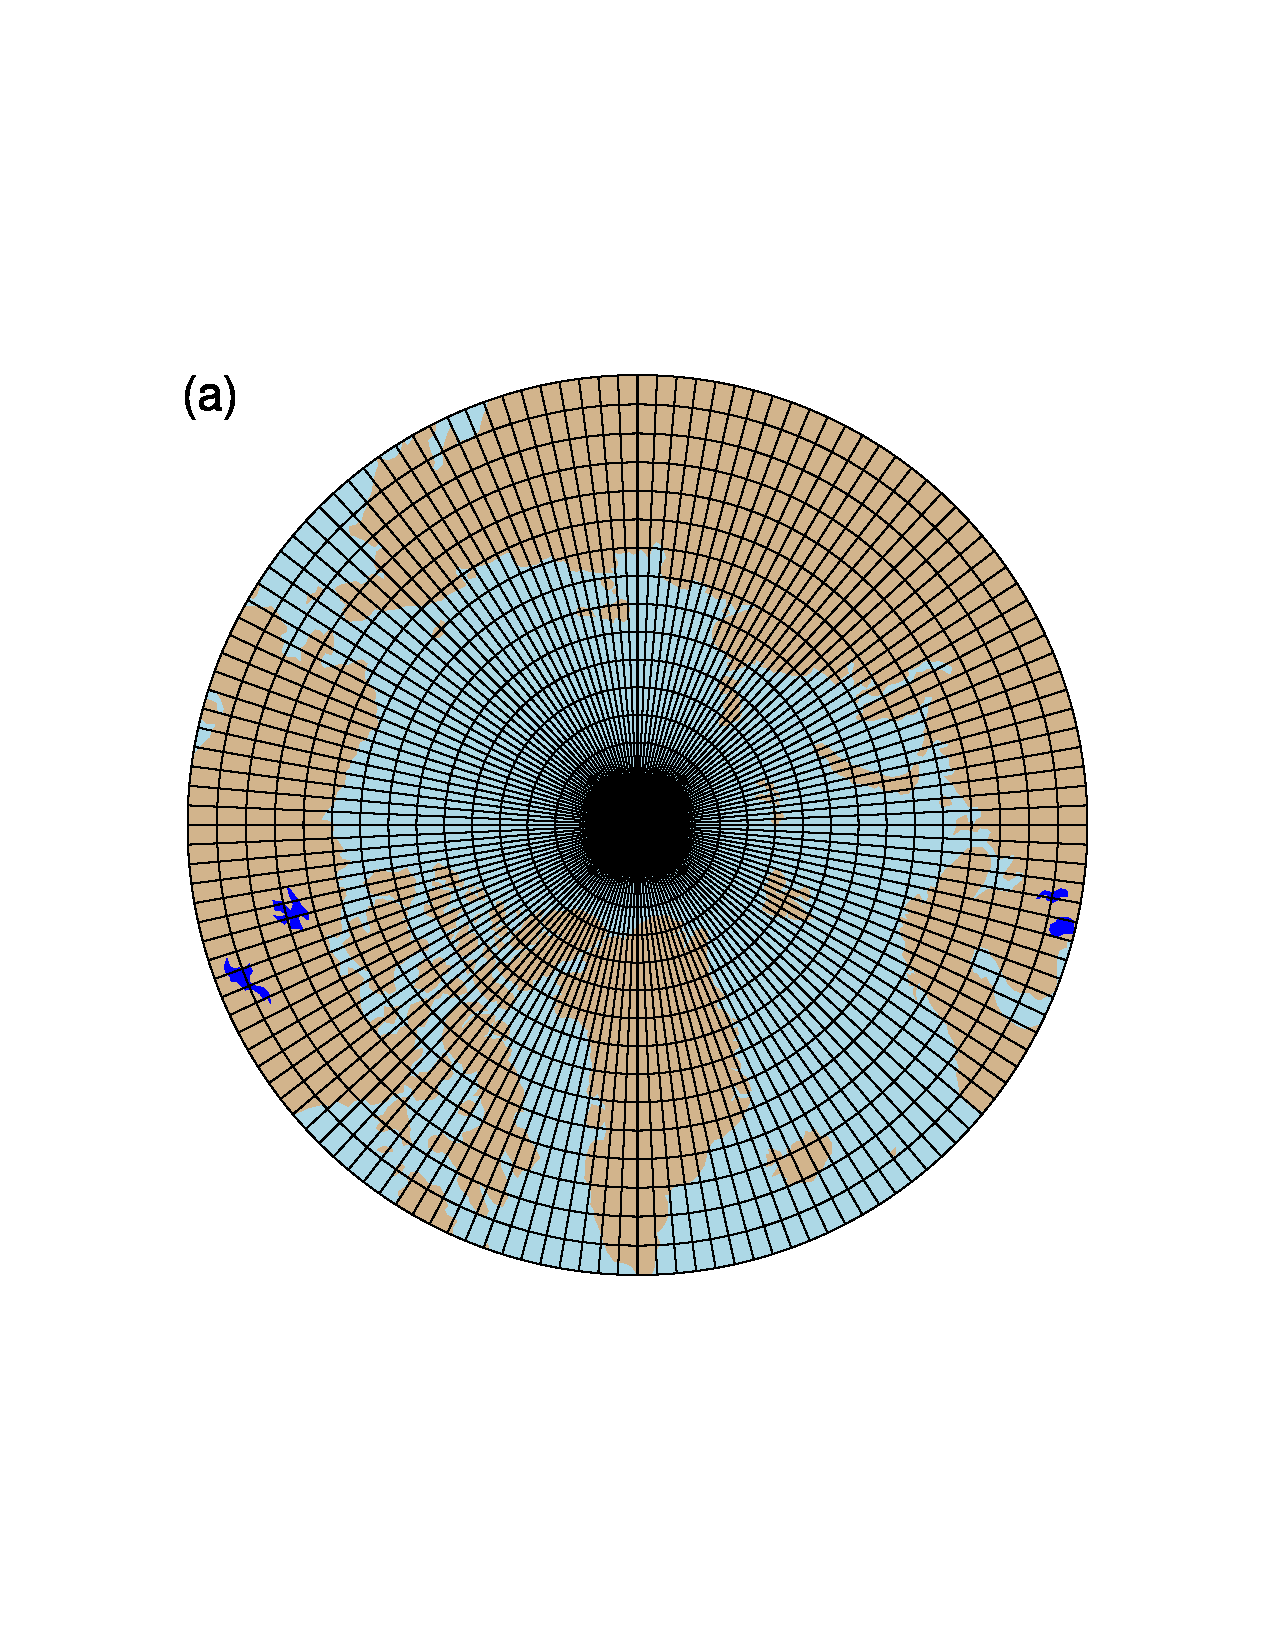
\includegraphics[width=60mm]{figs/grid-f19.pdf}&
         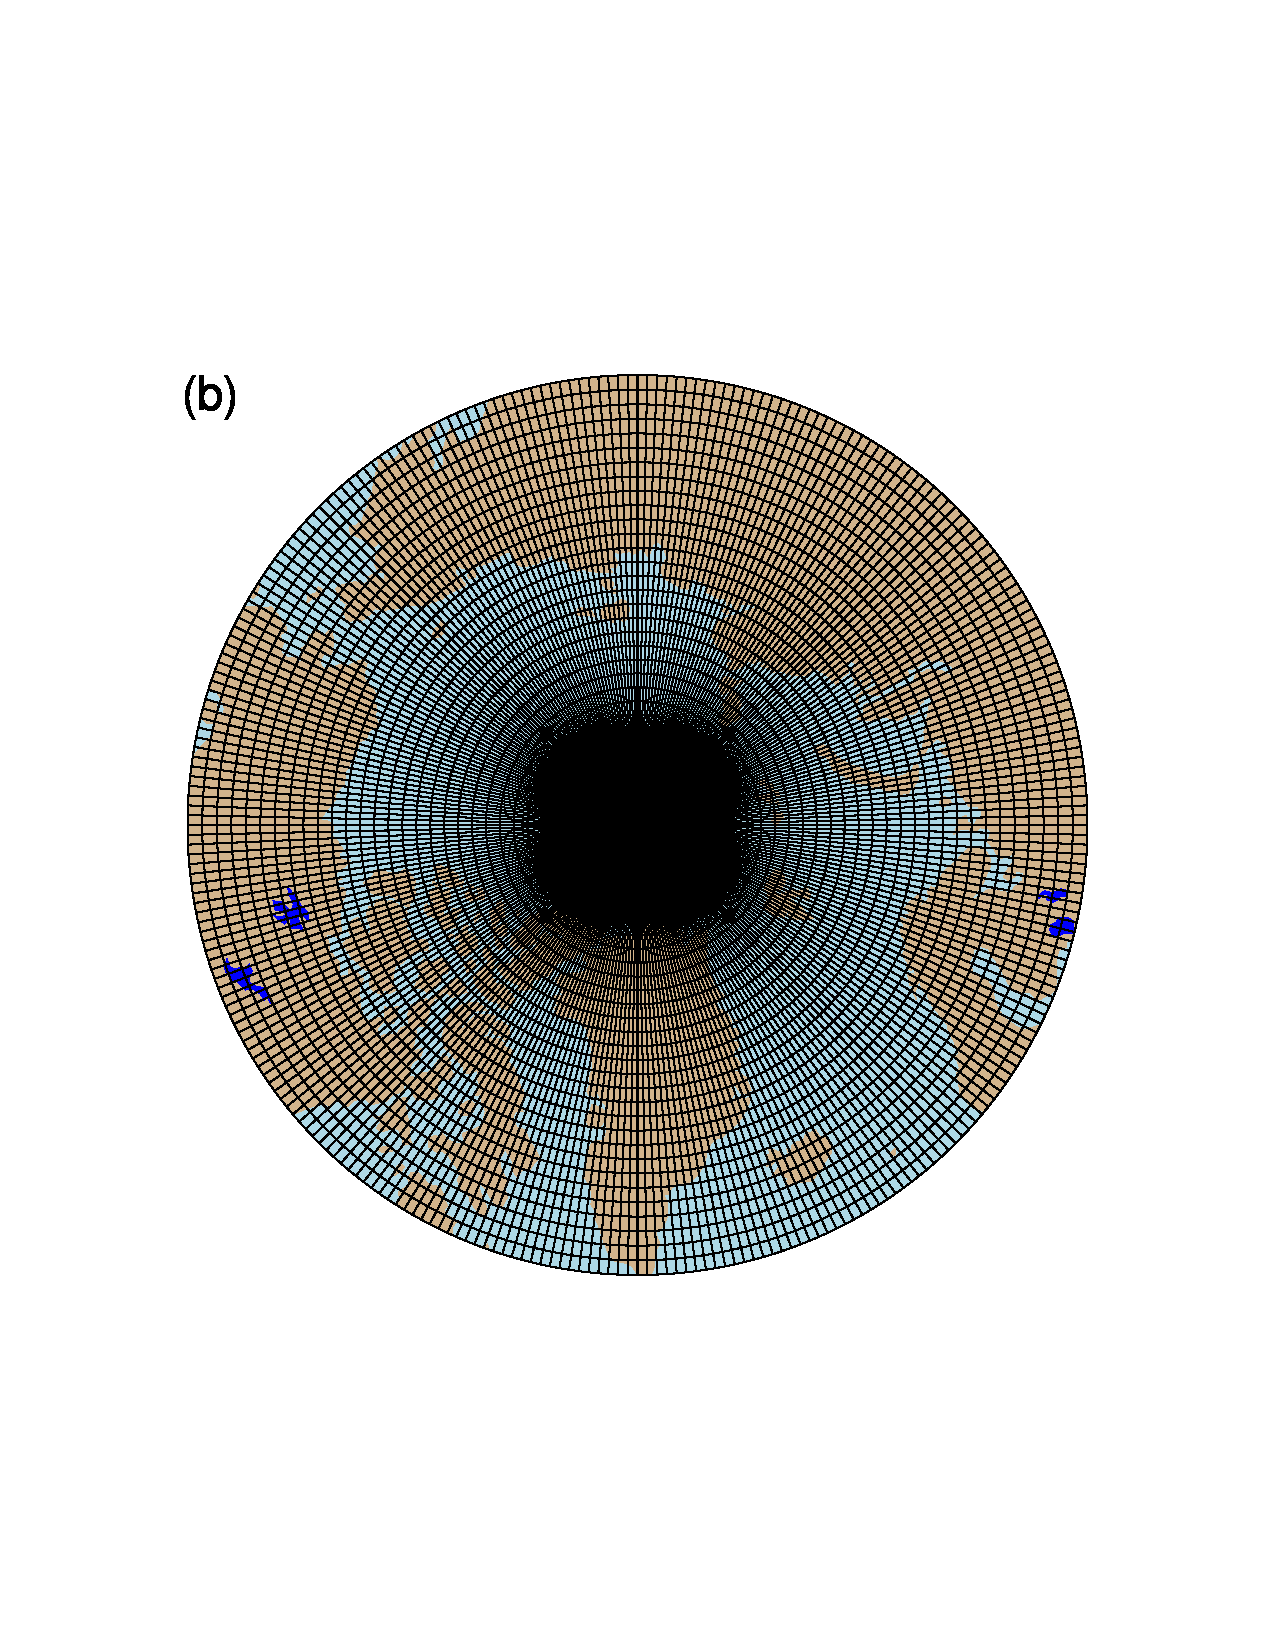
\includegraphics[width=60mm]{figs/grid-f09.pdf}\\
         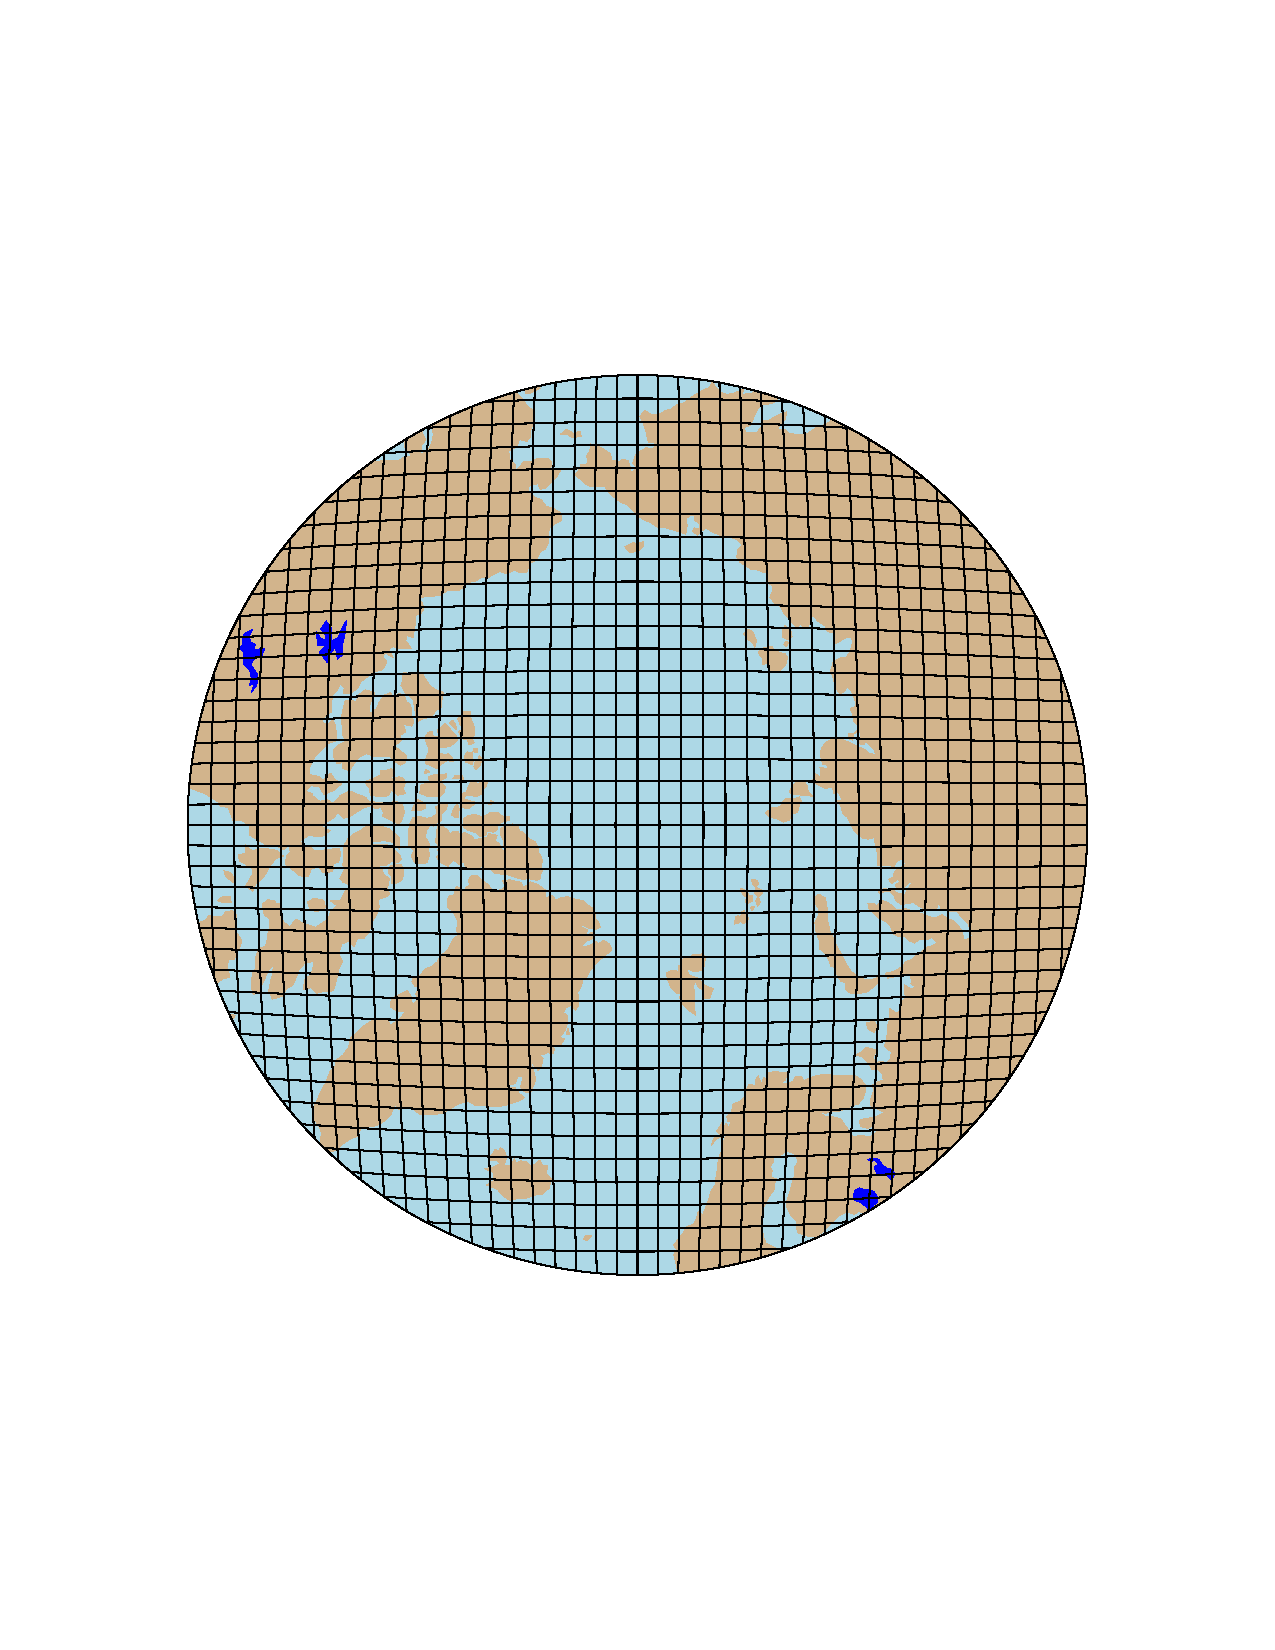
\includegraphics[width=60mm]{figs/grid-ne30pg2.pdf}&
         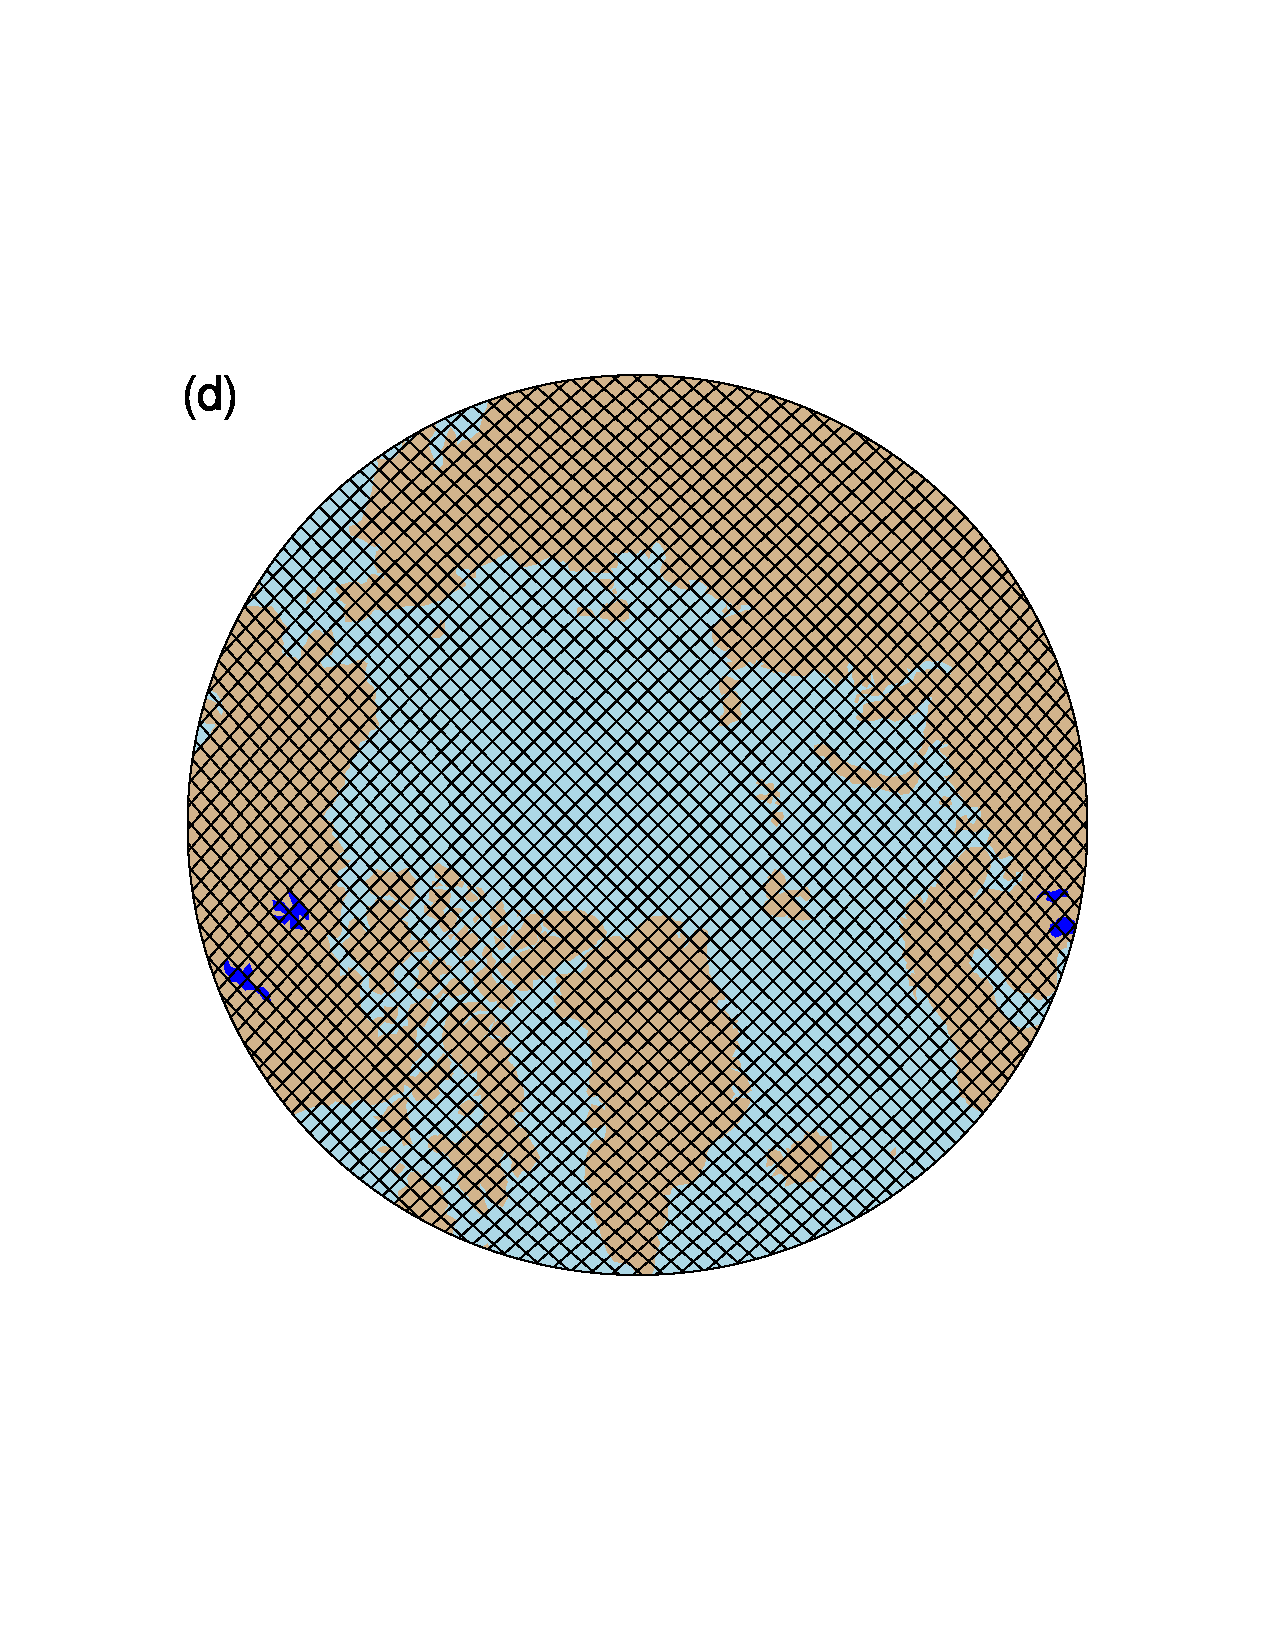
\includegraphics[width=60mm]{figs/grid-ne30pg3.pdf} \\
\end{tabular}
\end{center}
\caption{Computational grids for the uniform $1^{\circ}-2^{\circ}$ grids in this study. Grids names after Table~\ref{tbl:table1}, (a) $\tt f19$, (b) $\tt f09$, (c) $\tt ne30pg2$ and (d) $\tt ne30pg3$.}
\label{fig:uni-grids}
\end{figure}

\begin{figure}[t]
\begin{center}
\begin{tabular}{cccc}
         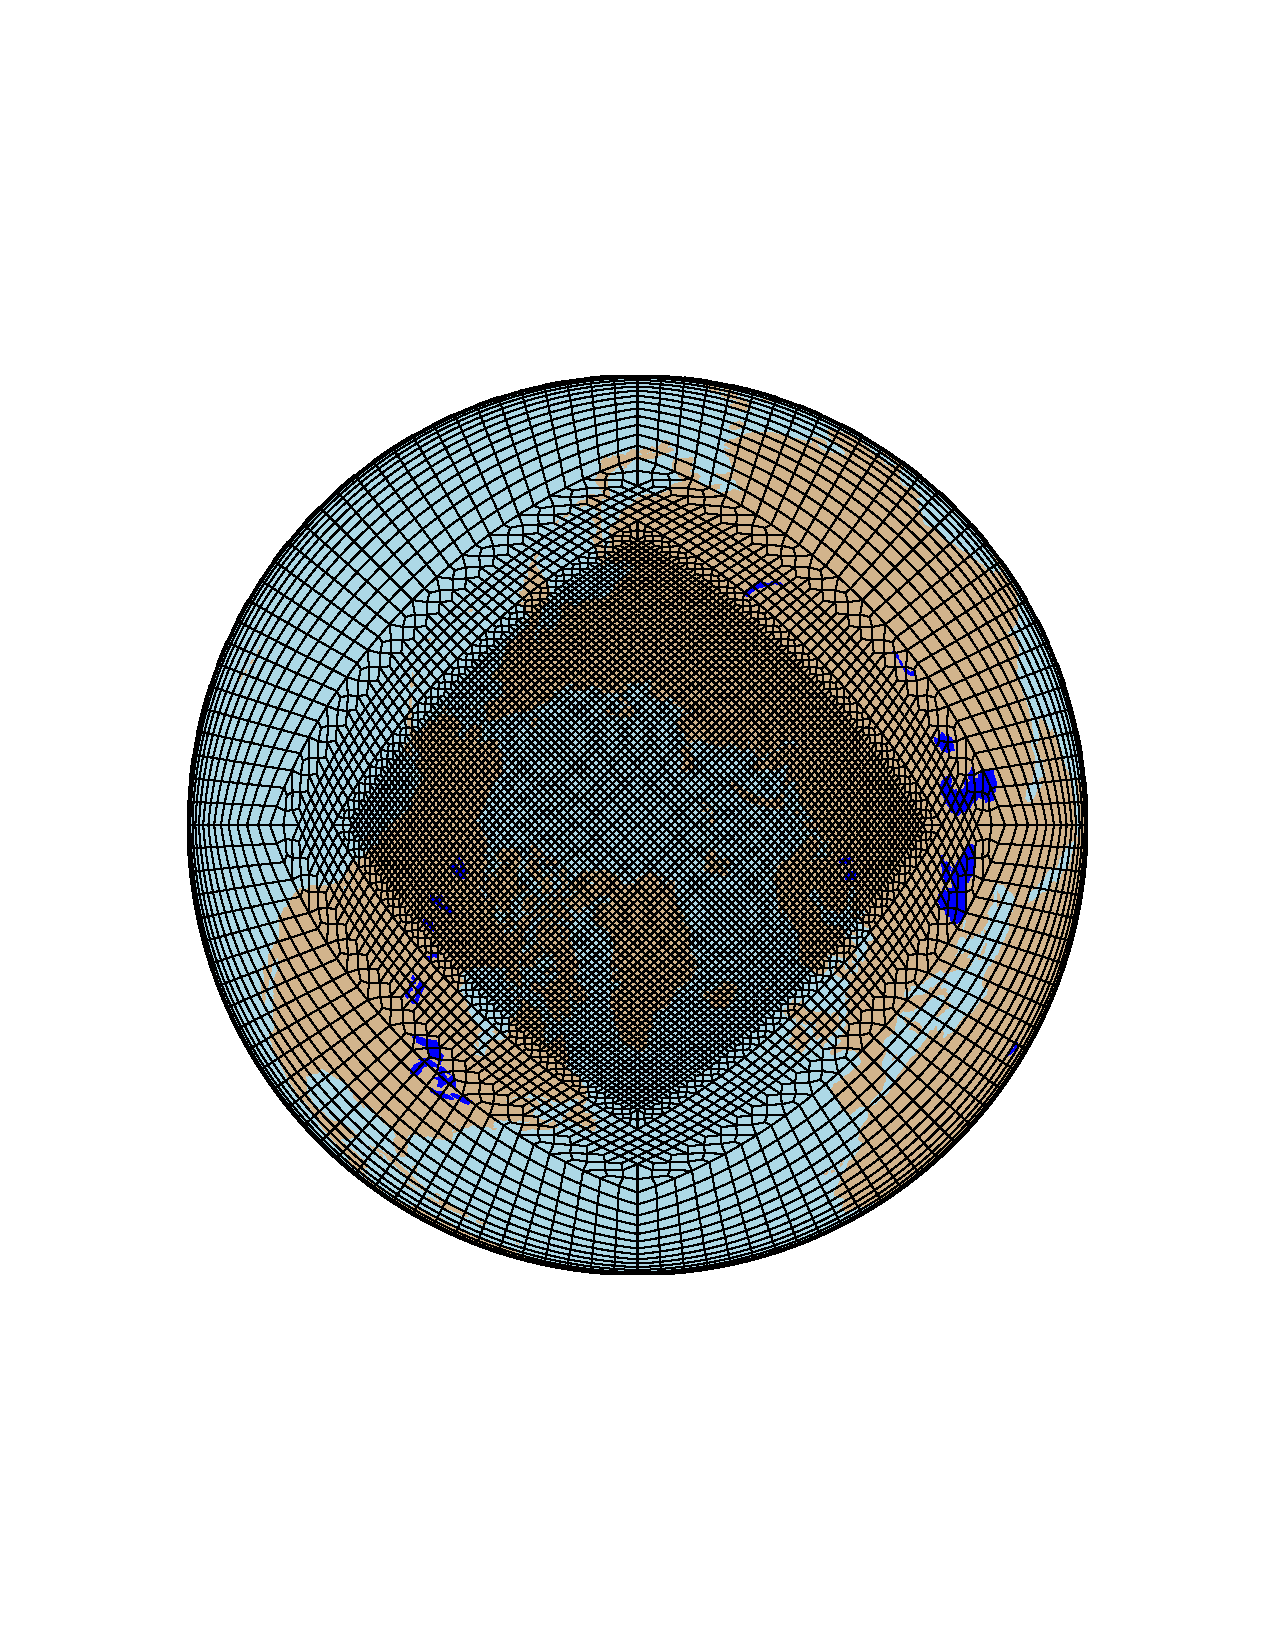
\includegraphics[width=60mm]{figs/grid-ARCTIC.pdf}&
         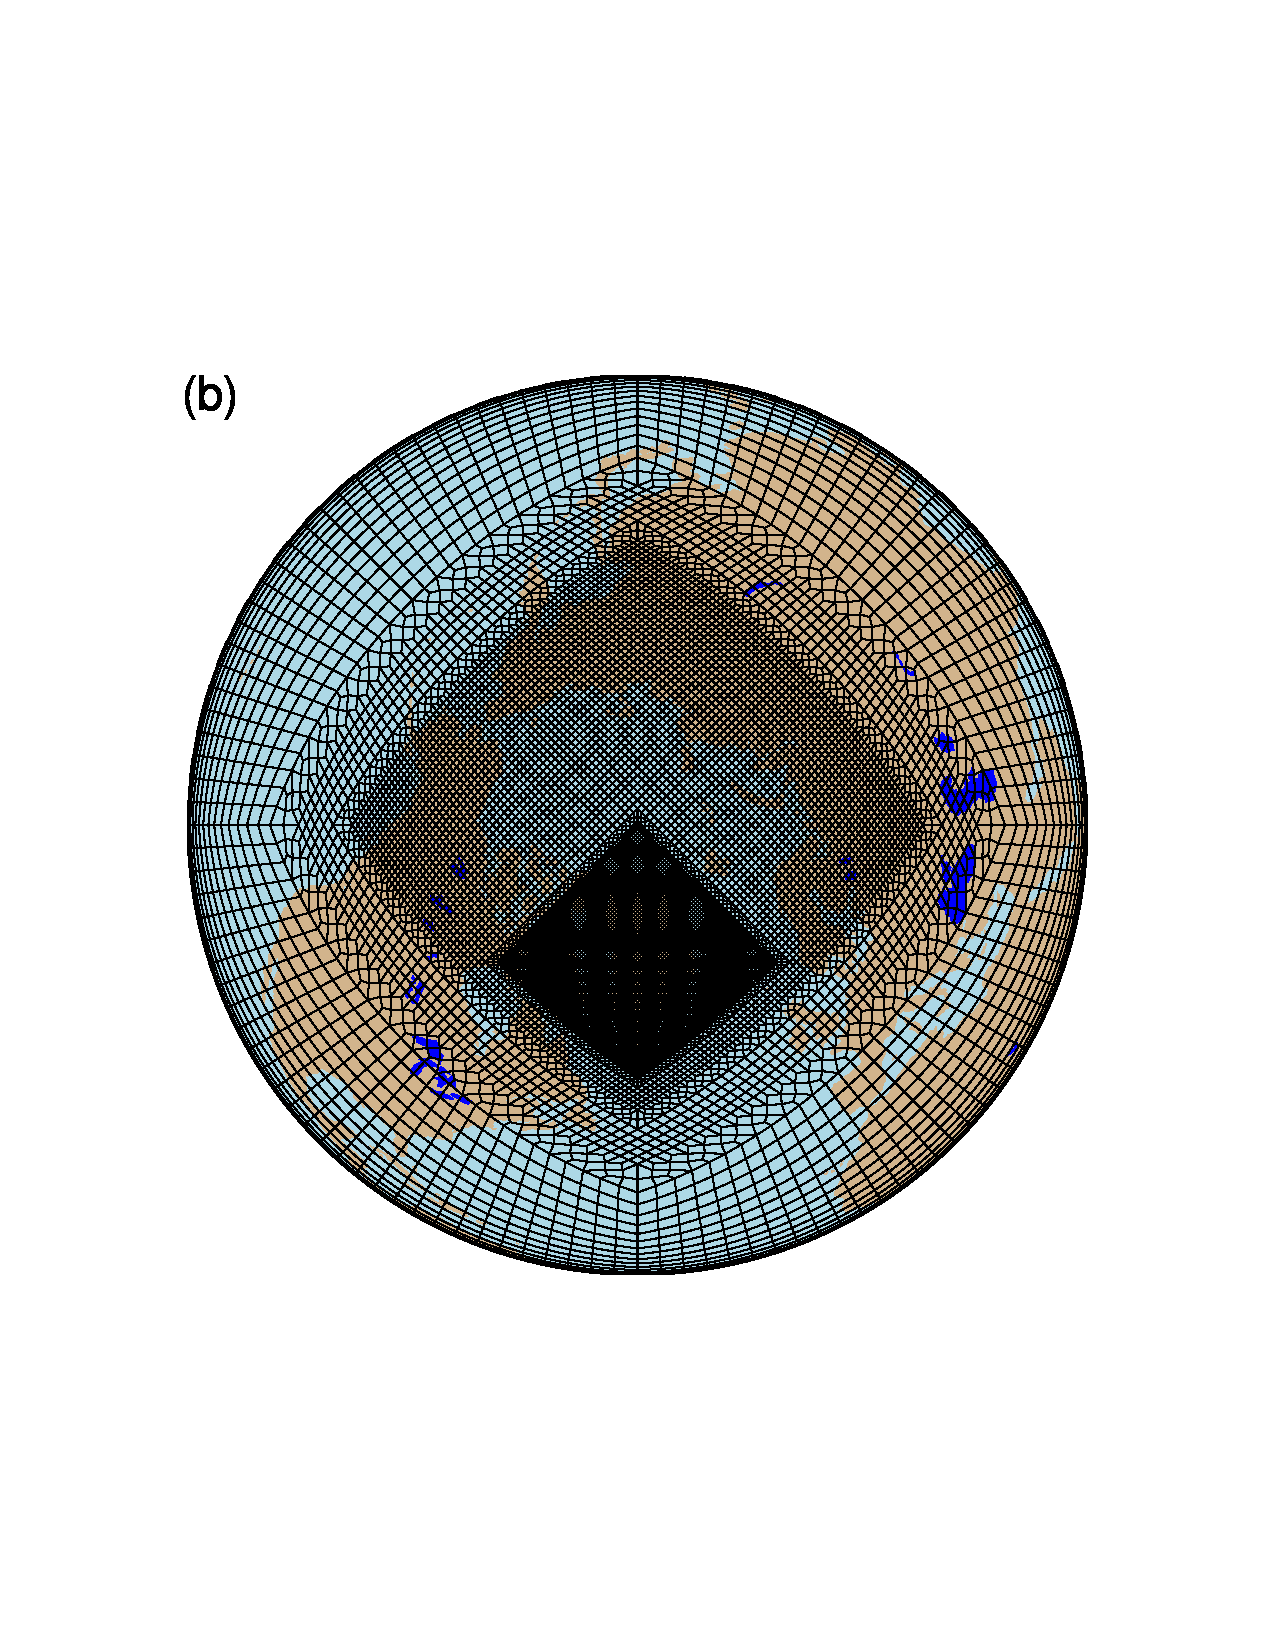
\includegraphics[width=60mm]{figs/grid-ARCTICGRIS.pdf} \\
\end{tabular}
\end{center}
\caption{Spectral-element grid for the VR grids in this study, (a)$\tt Arctic$, (b) $\tt Arctic-GrIS$ and (a) $\tt CONUS$. Note that this is not the computational grid; each element has $3\times3$ independent grid points. {\color{red}{add CONUS grid}}}
\label{fig:vr-grids}
\end{figure}

\section{Methods}\label{sec:methods}
\subsection{Dynamical cores}

The atmospheric component of CESM2.2 \cite{CESM2}, the Community Atmosphere Model, version 6.3 \cite<CAM;>{Gettelman2019GRL}, supports several different atmospheric dynamical cores. These include dycores on lat-lon grids, such as finite-volume \cite<FV;>{L2004MWR} and Eulerian spectral transform \cite<EUL;>{CETAL006JC} models, and dycores built on unstructured grids, including spectral-element \cite<SE;>{LetAl2018JAMES} and finite-volume 3 \cite<FV3;>{PL2007JCP} models. This study compares the performance of the SE and FV dycores, omitting the EUL and FV3 dycores {\color{green}{Andrew - maybe not mention EUL or FV3?}}.

[phl: maybe mention that FV was used for IPCC simulations; SE in iHESP]

\subsubsection{Finite-volume (FV) dynamical core}

The FV dycore is a hydrostatic model that integrates the equations of motion using a finite-volume discretization on a spherical lat-lon grid \cite{LR1997QJR}. The 2D dynamics evolve in floating Lagrangian layers that are periodically mapped to an Eulerian reference grid in the vertical \cite{L2004MWR}, using a hybrid-pressure vertical coordinate. Hyperviscous damping is applied to the divergent modes, while Laplacian damping is applied to momentum in the top few layers, referred to as a \textit{sponge layer} \cite{L2011IJHPC} [phl: as far as I know the Laplacian-like damping is not invoked in lower resolution setups - was implemented for 1/4 applications where the polar night jet became excessively strong]. A polar filter damps computational instability due to the convergence of meridians, allowing a longer time step. It takes the form of a Fourier filter in the zonal direction, with the damping coefficients increasing monotonically in the meridional direction \cite{ST1995GEOS}. The form of the filter is designed to slow down the propagation of large zonal wave-numbers to satisfy the CFL condition of the shortest resolved wave at some reference latitude.

\subsubsection{Spectral-element (SE) dynamical core}

The SE dycore is a hydrostatic model that integrates the equations of motion using a high-order continuous Galerkin method \cite{TTI1997JCP,TF2010JCP}. The computational domain is a cubed-sphere grid tiled with quadrilateral elements (see Figure~\ref{fig:vr-grids}). Each element contains a fourth-order basis set in each horizontal direction, with the solution defined at the roots of the basis functions, the Gauss-Lobatto-Legendre quadrature points. This results in 16 nodal points per element, with 12 of the points lying on the (shared) element boundary. Communication between elements uses the direct stiffness summation \cite{canuto2007}, which applies a numerical flux to the element boundaries to reconcile overlapping nodal values and produce a continuous global basis set. 

As with the FV dycore, the dynamics evolve in floating Lagrangian layers that are subsequently mapped to an Eulerian reference grid. A dry mass vertical coordinate was recently implemented for thermodynamic consistency with condensates \cite{LetAl2018JAMES}. The 2D dynamics have no implicit dissipation, and so hyperviscosity operators are applied to all prognostic variables to remove spurious numerical errors \cite{DetAl2012IJHPCA}. Laplacian damping is applied in the sponge layer.

The SE dycore supports regional grid refinement via its VR configuration, requiring two enhancements to uniform-resolution grids: (1) As the numerical viscosity increases with resolution, explicit hyperviscosity relaxes according to the local element size, reducing in strength  by an order of magnitude per halving of the grid spacing. A tensor-hyperviscosity formulation is used \cite{GetAl2014GMD}, which adjusts the coefficients in two orthogonal directions to more accurately target highly distorted quadrilateral elements. (2) The topography boundary conditions need to be smoothed in a way that does not excite grid scale modes, and so the NCAR topography software \cite{gmdd-8-4623-2015} has been modified to scale the smoothing radius by the local element size. 

For SE grids with quasi-uniform grid spacing, The SE tracer transport scheme is replaced with the Conservative Semi-Lagrangian Multi-tracer transport scheme (CSLAM) \cite<>{LTOUNGK2017MWR}. CSLAM has improved tracer property preservation and accelerated multi-tracer transport. It uses a separate grid from the spectral-element dynamics, dividing each element into $3\times3$ control volumes with quasi-equal area. The physical parameterizations are computed from the state on the CSLAM grid, which has clear advantages over the default SE dycore in which the physics are evaluated Gauss-Lobatto-Legendre points \cite{HL2018MWR}. {\color{purple}{Rene/Andrew - maybe elaborate further on the advantages of CSLAM?}}

\subsection{Grids}

We evaluate model simulations on six different grids in this study (Table~\ref{tbl:table1}). The FV dycore is run with nominal $1^{\circ}$ and $2^{\circ}$ grid spacing, referred to as $\tt f09$ and $\tt f19$, respectively (Figure~\ref{fig:uni-grids}a,b). We also run the $1^{\circ}$ equivalent of the CAM-SE-CSLAM grid, referred to as $\tt ne30pg3$ (Figure~\ref{fig:uni-grids}c), where $ne$ refers to a grid with of $ne \times ne$ elements per cubed-sphere face, and $pg$ denotes that there are $pg \times pg$  control volumes per element for computing the physics. We run an additional $1^{\circ}$ CAM-SE-CSLAM simulation with the physical parameterizations computed on a grid with $2\times2$ control volumes per element, $\tt ne30pg2$ \cite<Figure~\ref{fig:uni-grids}d; note CSLAM is still run on the $3\times3$ control volume grid;>{HETAL2019JAMES}.

Two VR meshes were developed for the CESM2.2 release to support grid refinement over the Arctic (Figure~\ref{fig:vr-grids}). This paper serves as the official documentation of these grids. The Arctic meshes were developed using the software package SQuadgen (\url{https://github.com/ClimateGlobalChange/squadgen}). The $\tt Arctic$ grid is a $1^{\circ}$ grid with $1/4^{\circ}$ regional refinement over the broader Arctic region. The $\tt Arctic-GrIS$ grid is identical to the $\tt Arctic$ grid, but with an additional patch covering the island of Greenland with $1/8^{\circ}$ resolution.

 \begin{table*}
 \centering
 \scriptsize
 \begin{tabular}{lccccc}
   \hline
   grid name & dycore & $\Delta x_{\mathrm{eq}}$ (km) & $\Delta x_{\mathrm{refine}}$ (km) & $\Delta t_{\mathrm{phys}}$ (s) \\ 
   \hline
   $\tt f19$ & FV & 278 & - &1800 \\
   $\tt f09$ & FV & 139 & - &1800 \\
   $\tt ne30pg2$ & SE-CSLAM & 167 & - & 1800 \\
   $\tt ne30pg3$ & SE-CSLAM & 111 & - & 1800 \\
   $\tt ne30pg3^{*}$ & SE-CSLAM & 111 & - & 450 \\
   $\tt Arctic$ & SE & 111 & 28 & 450 \\
   $\tt Arctic-GrIS$ & SE & 111 & 14 & 225 \\
 \hline
 \end{tabular}
  \caption{Grids and dycores used in this study. $\Delta x_{\mathrm{eq}}$ is the average equatorial grid spacing, $\Delta x_{\mathrm{refine}}$ is the grid spacing in the refined region (if applicable), and $\Delta t_{\mathrm{phys}}$ is the physics time step. FV refers to the finite-volume dycore, SE the spectral-element dycore, and SE-CSLAM the spectral-element dycore with CSLAM tracer advection.  We use the $\tt ne30pg3$ grid for two runs with different values of $\Delta t_{\mathrm{phys}}$.{\color{purple}{Rene - maybe include model cost?}}}
 \label{tbl:table1}
 \end{table*}

The physics time step depends on the grid resolution. Increased horizontal resolution permits faster vertical velocities that reduce characteristic time scales, so the physics time step is reduced to avoid large time truncation errors \cite{HR2018JAMES}. The $\tt Arctic$ and $\tt Arctic-GrIS$ grids are run with a $4\times$ and $8\times$ reduction in physics time step relative to the default 1800 s time step for the standard $1^{\circ}$ and $2^{\circ}$ grids (Table~\ref{tbl:table1}).

All grids and dycores in this study use 32 levels in the vertical, with a model top of about 1~hPa or 40~km. However, note that any grid or dycore can in principle be run with a higher model top or finer vertical resolution.

\subsection{Physical parameterizations}

All simulations in this study use the CAM6.3 physical parameterization package \cite<hereafter referred to as the \textit{physics};>{Gettelman2019GRL}. The physics in CAM6 differs from its predecessors through the incorporation of high-order turbulence closure, Cloud Layers Unified by Binormals \cite<CLUBB;>{GETAL2002JAS,BOG2013JCLIM}, which jointly acts as a planetary boundary layer, shallow convection, and cloud macrophysics scheme. CLUBB is coupled with the MG2 microphysics scheme \cite{MG2,Morrison2015}, with prognostic precipitation and classical nucleation theory to represent cloud ice for improved cloud-aerosol interactions. Deep convection is parameterized using a convective quasi-equilibrium, bulk plume mass flux scheme \cite{ZM1995AO,NRJ2008JC} and includes convective momentum transport \cite{RSG2010JAS}. Boundary layer form drag is modeled after \citeA{BBW2004QJRMS}, and orographic gravity wave drag is represented with an anisotropic method informed by the orientation of topographic ridges at the sub-grid scale (the ridge orientation is derived from a high-resolution, global topography dataset \cite{Danielson_Gesch_2011_GMTED2010}). 

Initial simulations with the $\tt ne30pg3$ SE grid produced weaker shortwave cloud forcing relative to the tuned finite-volume dycore. The SE dycore in CESM2.2 therefore has two CLUBB parameter changes to provide more realistic cloud forcing and top-of-atmosphere radiation balance. We reduced the width of the sub-grid distribution of vertical velocity ($\tt clubb_gamma$ is reduced from 0.308 to 0.270) and also reduced the strength of the damping for horizonatal component of turbulent energy ($\tt clubb_c14$ is reduced from 2.2 to 1.6) to increase cloudiness. For a thorough explanation of how CLUBB parameters impact the simulated climate, see \cite{GETAL2015JAMES}.

\subsection{Experimental design}

All simulations described here use an identical transient 1979-1998 Atmospheric Model Inter-comparison Project (AMIP) configuration, with prescribed monthly sea-surface temperature and sea ice following \citeA{CESMSST}. In CESM terminology, AMIP simuations use the $FHIST$ computational set and run out of the box in CESM2.2. {\color{orange}{Marcus - this is the only part that doesn't talk about CLM/CISM coupling. Move somewhere else and change section name?}}

All grids and dycores simulate the GrIS Surface Mass Balance (SMB). The SMB is the sum of mass accumulation of precipitation and mass loss from ablation. Ablation is the sum of evaporation/sublimation and liquid runoff, with runoff being a combination of liquid precipitation and snow and ice melt. Not all liquid precipitation runs off the ice sheet; liquid runoff (which is composed of both rain or ice/snow melt) can penetrate pore spaces in the snowpack/firn layer and freeze, increasing the ice mass. These processes are represented by different CESM components, but it is the Community Land Model, version 5 \cite<CLM;>{CLM5}, that aggregates these processes and computes the SMB.

CLM runs on the same grid as the atmosphere, using a downscaling technique to account for sub-grid variability in SMB. In short, the ice sheet patch in a CLM grid cell is subdivided into 10 elevation classes (ECs), each with a distinct surface energy balance and SMB. The area fraction of each EC is derived from a high-resolution GrIS elevation dataset. The near-surface air temperature, humidity, and air density are calculated for each EC using an assumed lapse rate and the elevation difference from the grid-cell mean. Precipitation from CAM is repartitioned into solid or liquid based on the surface temperature of the EC; precipitation falls as snow for temperatures between $T < -2^\circ$~C, as rain for $T > 0^\circ$~C,  and as a linear combination of rain and snow for temperatures between $-2^\circ$~C and $0^\circ$~C.
Snow accumulation in each EC is limited to a depth of 10 m liquid water equivalent. Any snow above the 10-m cap is routed to the ocean as solid runoff.  Refreezing of liquid water within the snowpack is an additional source of ice.  Integrating over all ECs, weighting by the area fractions, provides a more accurate SMB than would be found using the grid-cell mean elevation. For a more detailed description of how the SMB is computed in CESM, we refer the reader to \citeA{Muntjewerf_EA_2021_coupling,CISM1,SETAL2019TC,KETAL2020JAMES}. {\color{orange}{Marcus - mention you're not running CISM.}}

Changes in ice depth, but not snow depth, count toward the SMB.  That is, snow accumulation above the 10-m cap contributes a positive SMB, and surface ice melting (after melting of the overlying snow) yields a negative SMB.  Since snow in the accumulation zone must reach the cap to simulate a positive SMB, the snow depths on the VR grids were spun up by forcing CLM in standalone mode, cycling over a 20-year $\tt Arctic$ $FHIST$ run for about 500 years. The uniform-resolution grids are initialized with the SMB from an existing $\tt f09$ spun-up initial condition.

\subsection{Observational Datasets}

We use several observational datasets (Table~\ref{tbl:table2}) to assess the performance of the simulations. We gathered SMB datasets from several sources. RACMO2.3 11km and RACMO2.3p2 5.5km are regional model simulations targeting Greenland, forced by ERA40, ERA interim, and ERA5 renalysis products at the domain boundaries. The Regional Atmospheric Climate Model (\textit{RACMO}) simulations have been shown to perform skillfully against observations and are often used as modeling targets \cite{NETAL2015TC,NETAL2019SCIENCE}. 

In-situ SMB (snow pit and ice cores) and radar accumulation datasets (e.g., IceBridge) are maintained in The Land Ice Verification and Validation toolkit (LIVVkit), version 2.1 \cite{LIVVkit}. However, these point-wise measurements are difficult to compare to model output spanning several different grids, especially since the SMB from each elevation class is not available from the model output. We used a nearest-neighbor technique for an initial analysis, which showed that the model biases are similar to those computed using the RACMO datasets. Because of the uncertainty of comparing gridded fields to point-wise measurements, and the lack of information added with regard to model biases, we omitted these datasets from our analysis. {\color{purple}{Andrew - maybe do show them, briefly?}}

 \begin{table*}
 \centering
 \scriptsize
 \begin{tabular}{lcccc}
   \hline
   data product & years used in this study & resolution & citation \\ 
   \hline
   ERA5 & 1979-1998 & $1/4^{\circ}$ & \citeA{ERA5} \\
   CERES-EBAF ED4.1 & 2003-2020 & $1^{\circ}$ & \citeA{CERES-EBAF} \\
   CALIPSO-GOCCP & 2006-2017 & $1^{\circ}$ & \citeA{CALIPSO-GOCCP} \\
   RACMO2.3 & 1979-1998 & 11 km & \citeA{NETAL2015TC} \\
   RACMO2.3p2 & 1979-1998 & 5.5 km & \citeA{NETAL2019SCIENCE} \\
 \hline
 \end{tabular}
  \caption{Description of observational datasets used in this study.}
 \label{tbl:table2}
 \end{table*}

\subsection{SMB Analysis}\label{sec:SMB}

We seek to integrate SMB components over a GrIS ice mask and to diagnose their contributions to the GrIS mass budget. However, the ice masks vary across the grids, especially in comparison to the RACMO3.2 ice mask, whose total area is about $3\%$ less than that of the reference dataset (Figure~\ref{fig:grisdx}). The area errors in Figure~\ref{fig:grisdx} may not seem large, but even $1-2\%$ area differences can lead to large differences in integrated SMB \cite{HETAL2022TC}. CLM's dataset creation tool generates the model ice mask by mapping a high-resolution dataset to the target grid using the Earth System Modeling Framework (ESMF) first-order conservative remapping algorithm \cite<ESMF;>{ESMF}. The figure suggests that the mapping errors are less than $1.5\%$ across the CESM2 grids.

\begin{figure}[t]
\begin{center}
         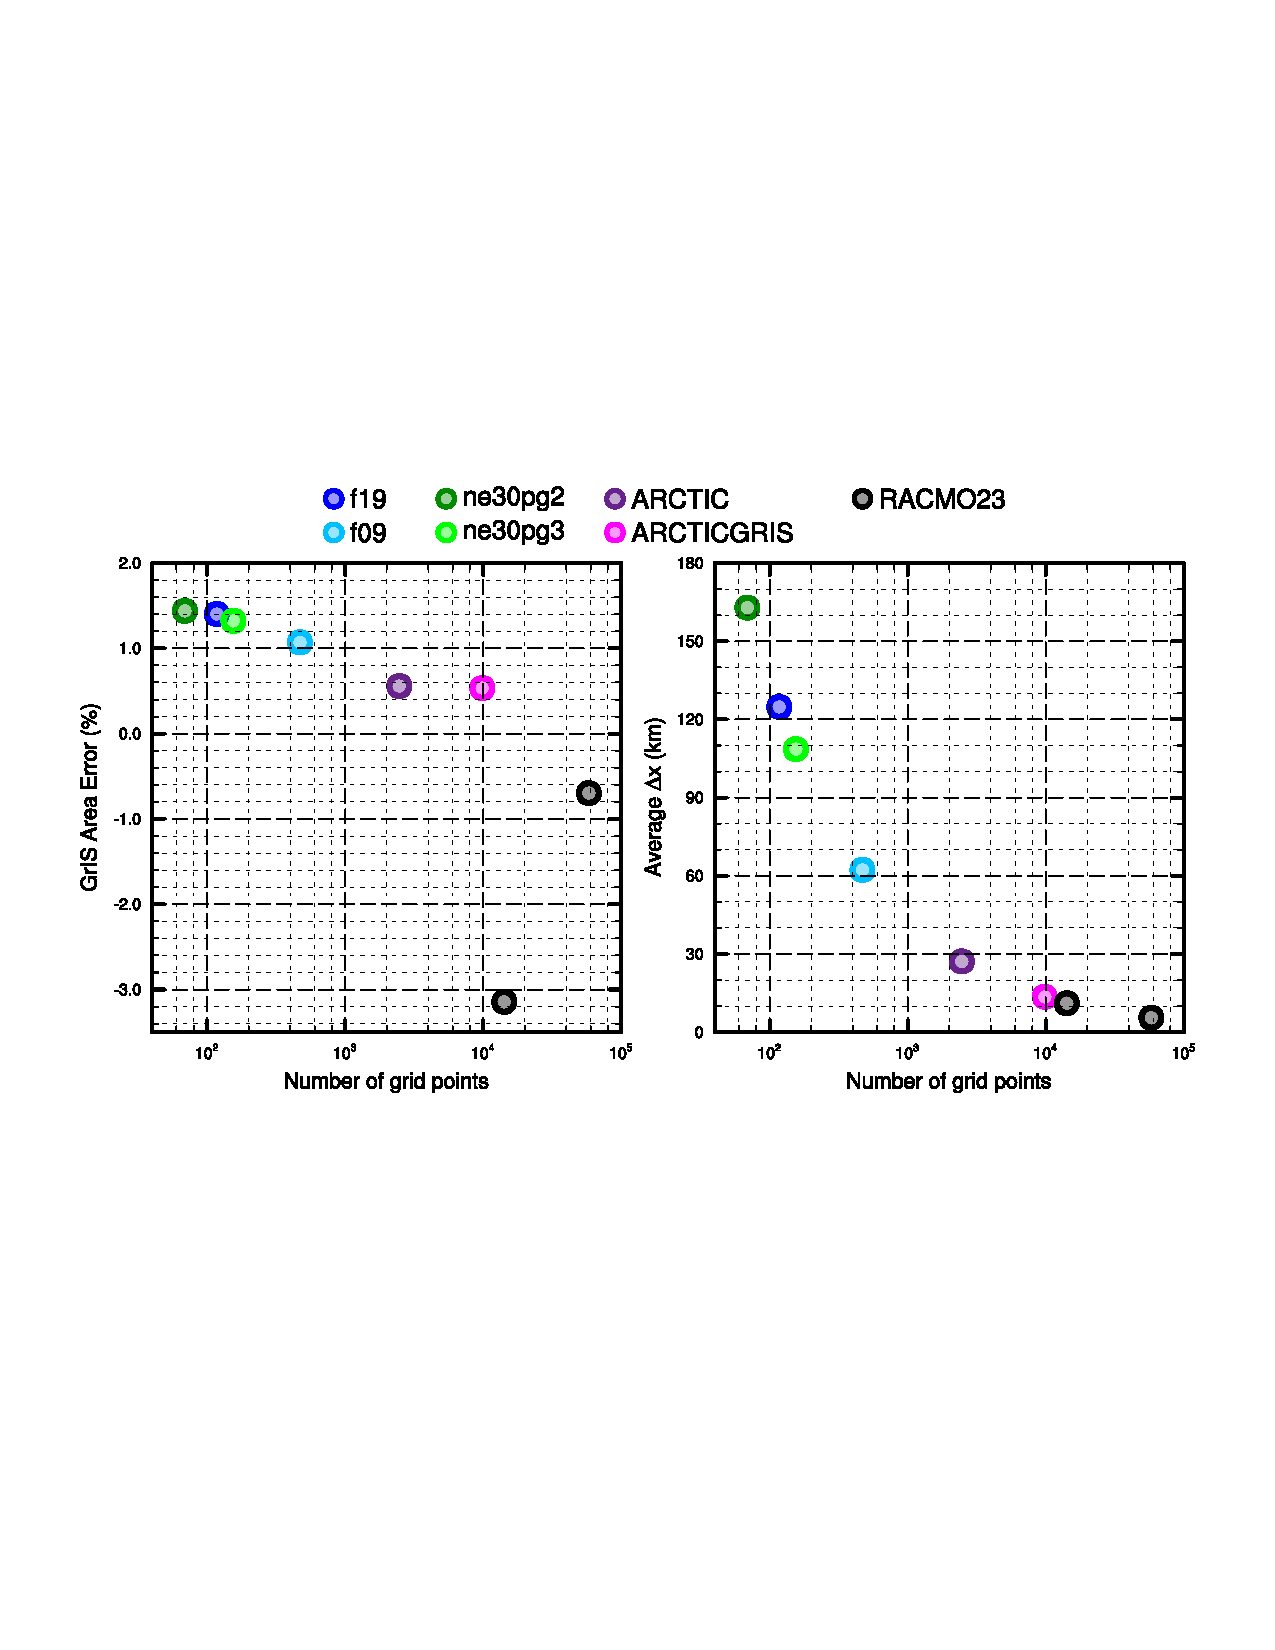
\includegraphics[width=100mm]{figs/temp_grisres.pdf}
\end{center}
\caption{The spatial properties of the GrIS as represented by different grids in this study. (Left) GrIS area error, computed as the relative differences from a 4km dataset used to create the CESM ice masks, (right) approximate average grid spacing over GrIS.}
\label{fig:grisdx}
\end{figure}

We have taken a common-ice-mask approach by mapping all model fields to the lowest-resolution grids, i.e., the $\tt f19$ and $\tt ne30pg2$ grids, and integrating over these low-resolution ice masks. The use of low-resolution common ice masks is a conservative decision and is largely because we seek to use first-order remapping algorithms to map fields to the common ice mask, which is not reliable in the downscaling direction, i.e., mapping to a higher-resolution grid than the source grid. We use two remapping algorithms: ESMF first-order conservative and the TempestRemap \cite{TempestRemap} high-order monotone algorithm. Since mapping errors are sensitive to grid type, we evaluate all quantities on both common ice masks, the $\tt f19$ and $\tt ne30pg2$ masks. Thus, we evaluate an integrated quantity on a given grid up to four times to estimate the uncertainty due to differences in grid type and remapping algorithms.

The SMB is expressed in a form that is agnostic of water phase, a total water mass balance, to facilitate comparisons across different grids with different ice masks and to increase consistency with the variables available in the RACMO datasets. The SMB for total water can be expressed as:
\begin{equation}
SMB = precipitation + runoff + evaporation/sublimation, \label{eq:SMB}
\end{equation}
where all terms have consistent sign conventions (positive values contribute mass, negative values reduce mass). The precipitation source term refers to the combined solid and liquid precipitation, runoff refers to the liquid water sink, and evaporation/sublimation is the vapor sink. Since the runoff term aggregates many processes, we isolate the melting contribution by also tracking the combined snow plus ice melt. Note that this SMB expression is different from the internally computed SMB in CLM \cite{KETAL2020JAMES}.

We consider two approaches for mapping and integrating the SMB components over the common ice masks:
\begin{enumerate}
\item Map the grid-cell mean quantities to the common grid, and integrate the mapped fields over the common ice masks. \label{lbl:label1}
\item Map the patch-level quantities (i.e., the state over the ice fractional component of the grid cell) to the common grid, and integrate the mapped fields over the common ice masks. \label{lbl:label2}
\end{enumerate}

Note that we are mapping to low-resolution grids that have larger GrIS areas (Figure~\ref{fig:grisdx}). Since the components of equation~\ref{eq:SMB} are not confined to the ice mask, method~\ref{lbl:label1} reconstructs the SMB over the portion of the common ice mask that is outside the ice mask on the source grid. While this may be a an acceptable way to reconstruct the mass source terms over different ice masks, ice melt is zero outside the source ice mask, and so method~\ref{lbl:label1} will underestimate the mass sink term. This underestimation is systematic in method~\ref{lbl:label2}; all variables are exclusive to the ice mask. Method~\ref{lbl:label2} is more dissipative, since mapping to the low-resolution grid will average a field of non-zero values over the ice mask with a field of zeros outside the ice mask. However, patch-level values for processes exclusive to the ice mask (e.g., ice melt) will on average have larger magnitudes than the the grid-mean quantities used in method~\ref{lbl:label1}. %The dilution of the these patch level fields caused by mapping to the common ice mask are then inflated due to integrating over the larger ice mask.

The different error characteristics of the two methods are used to diversify the ensemble. Each of the four regridding combinations (with conservative and high-order remapping to the $\tt f09$ and $\tt ne30pg2$ grids) are repeated with each method, resulting in (up to) eight values for each integrated quantity. Unfortunately, the patch-level values of evaporation/sublimation are not available from the model output, and we estimate their contribution by zeroing out the field for grid cells that have no ice, prior to mapping to the common ice mask. This will degrade the SMB estimates using method~\ref{lbl:label2}, but note that we are more interested in the behavior of the processes across grids and dycores, expressed as the components of the SMB, rather than the SMB itself.

\section{Results}\label{sec:results}

\subsection{Tropospheric temperatures}

Before delving into the simulated Arctic, we assess the global mean differences between the various grids and dycores. Figure~\ref{fig:dT-lores} shows 1979-1998 annual mean, zonal mean height plots expressed as differences between uniform-resolution grids and dycores. The $\tt f09$ grid is warmer than the $\tt f19$ grid, primarily in the mid-to-high latitudes throughout the depth of the troposphere. This is a common response to increasing horizontal resolution in GCMs \cite{PS2002CD,RETAL2006JC}.
\citeA{HK2020QJRMS} have shown that this occurs in CAM due to greater resolved vertical velocities which, in turn, drive more condensational heating in the CLUBB macrophyiscs. The right columns in Figure~\ref{fig:dT-lores} support this interpretation, showing an increase in the climatological CLUBB heating in low ({\color{blue}{looks more like subtropics}}) and mid-latitudes on the $\tt f09$ grid. 

\begin{figure}[t]
\begin{center}
         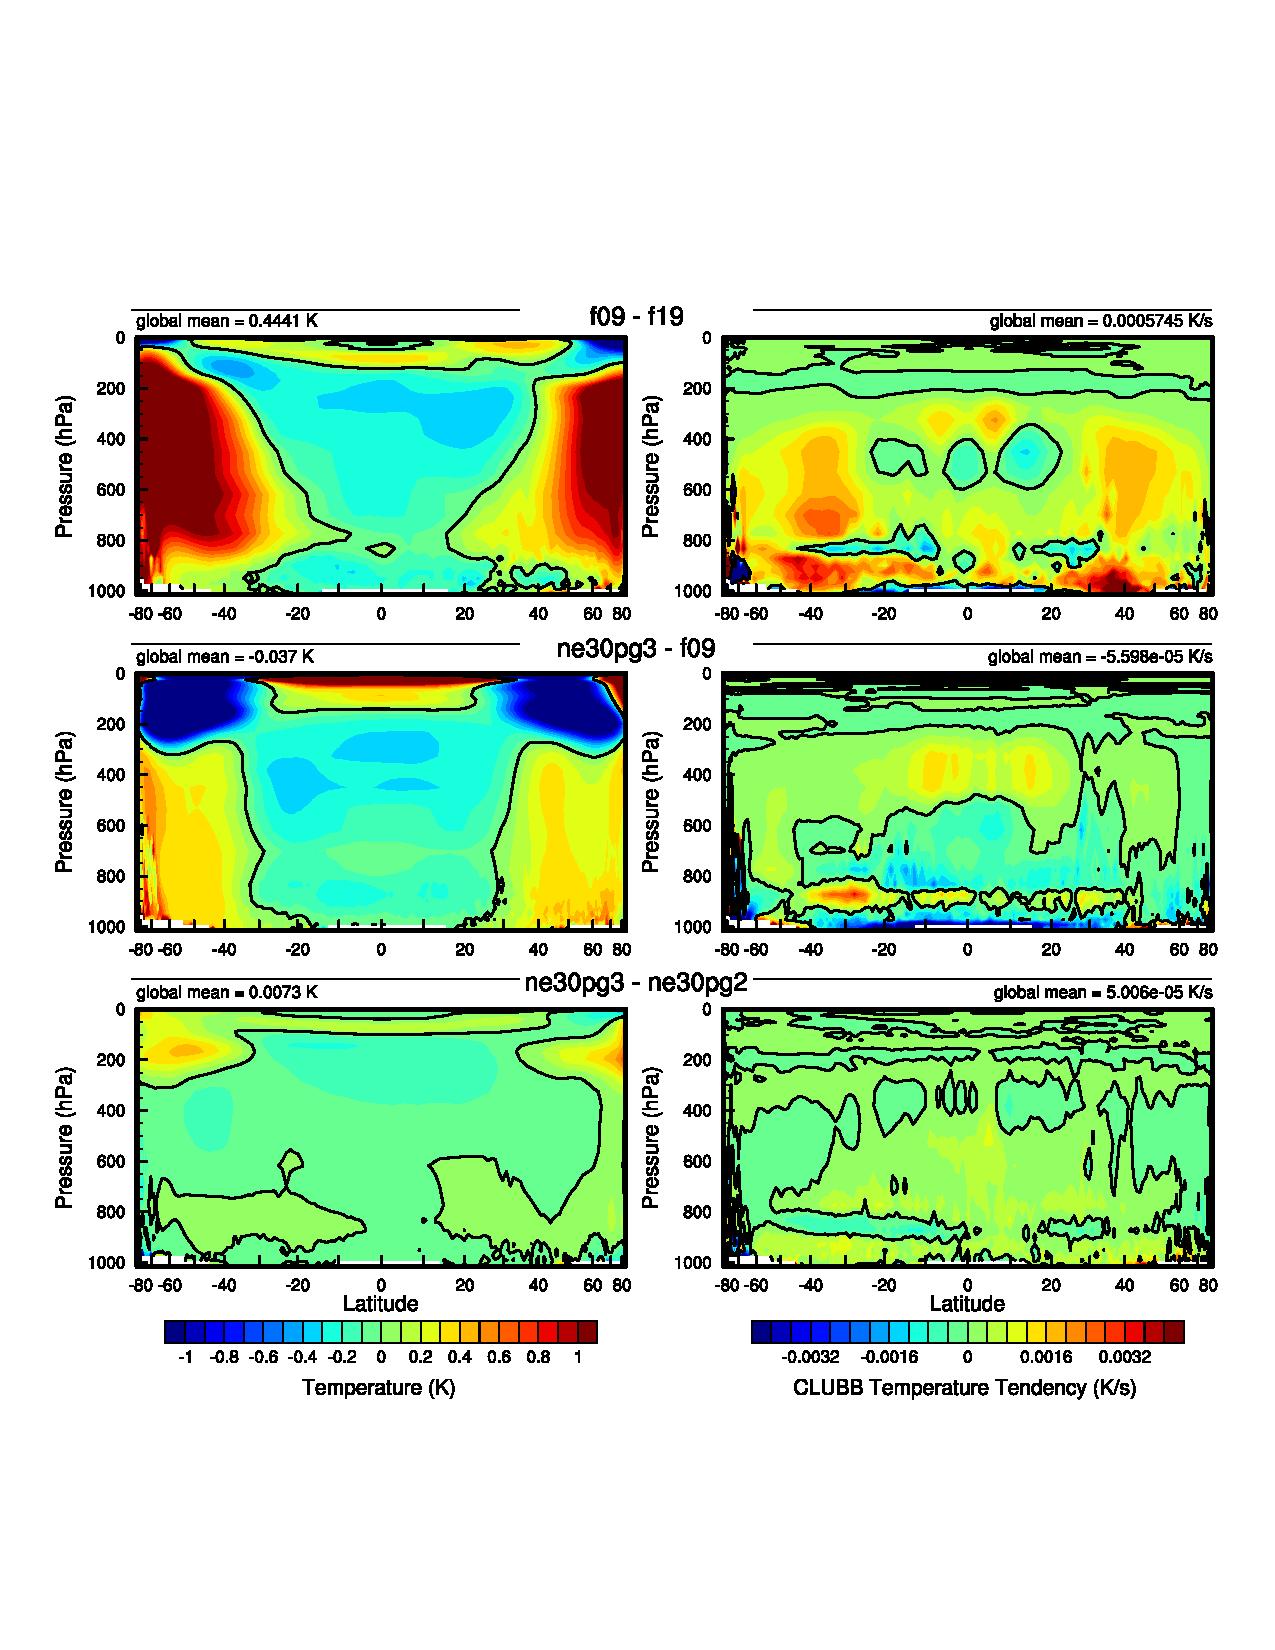
\includegraphics[width=130mm]{figs/temp_dhgt_panel_STEND_CLUBB-lores.pdf}
\end{center}
\caption{1979-1998 annual mean temperature (left column) and CLUBB temperature tendencies (right column) in zonal mean height space, expressed as differences between the various $1^{\circ}-2^{\circ}$ grids. The thick grey and magenta lines are the tropopause for the control run and the test run, respectively.}
\label{fig:dT-lores}
\end{figure}

As the SE dycore is less diffusive than the FV dycore, the resolved vertical velocities are larger in the SE dycore, and so the $\tt ne30pg3$ troposphere is modestly warmer than $\tt f09$ (Figure~\ref{fig:dT-lores}). The stratosphere responds differently, with $\tt ne30pg3$ much cooler than $\tt f09$ in the mid-to-high latitudes. Figure~\ref{fig:dT-lores} also shows small temperature differences between $\tt ne30pg3$ and $\tt ne30pg2$, with  $\tt ne30pg3$ slightly warmer near the tropopause at high latitudes. This is consistent with the similar climates found for these two grids by \citeA{HETAL2019JAMES}.

Comparing the VR grids to the uniform-resolution grids is complicated because we simultaneously increase the resolution and reduce the physics time-step, both of which impact the solution \cite{W2008TELLUS}. We therefore run an additional $\tt ne30pg3$ simulation with the shorter physics time step used in the $\tt Arctic$ grid (450~s), referred to as $\tt ne30pg3^{*}$. Figure~\ref{fig:dT-hires}a shows the difference between $\tt ne30pg3^{*}$ and $\tt ne30pg3$ for climatological summer temperatures in zonal-mean height space. Much of the troposphere is warmer with the reduced time step, and the mechanism is similar in that the shorter time step increases condensational heating by CLUBB. Figure~\ref{fig:dT-hires}b shows the difference in climatological summer temperature between the $\tt Arctic$ grid and the $\tt ne30pg3^{*}$ grid.  With the same physics time step on each grid, the greater condensational heating and warmer temperatures are confined to the refined Arctic region.

Figure~\ref{fig:dT-hires}c shows that the $\tt Arctic-GrIS$ grid is much warmer than the $\tt Arctic$ grid in the Arctic summer. This may be due, in part, to the shorter physics time step,
%; a similar physics-time-step sensitivity in the $\tt ne30pg3^{*}$ comparison is evident in the CLUBB tendencies in the $ARCTCGRIS$ grid.
but the temperature response is too large to be explained by the CLUBB changes alone. This summer warming appears to be a result of variations in the stationary wave pattern, with anomalous southerly winds to the west of Greenland (not shown). This dynamic response is interesting, because other than the physics time step, the only difference between the $\tt Arctic-GrIS$ and $\tt Arctic$ runs is the doubling of resolution over Greenland. This behavior will be explored further in a future study.

\begin{figure}[t]
\begin{center}
         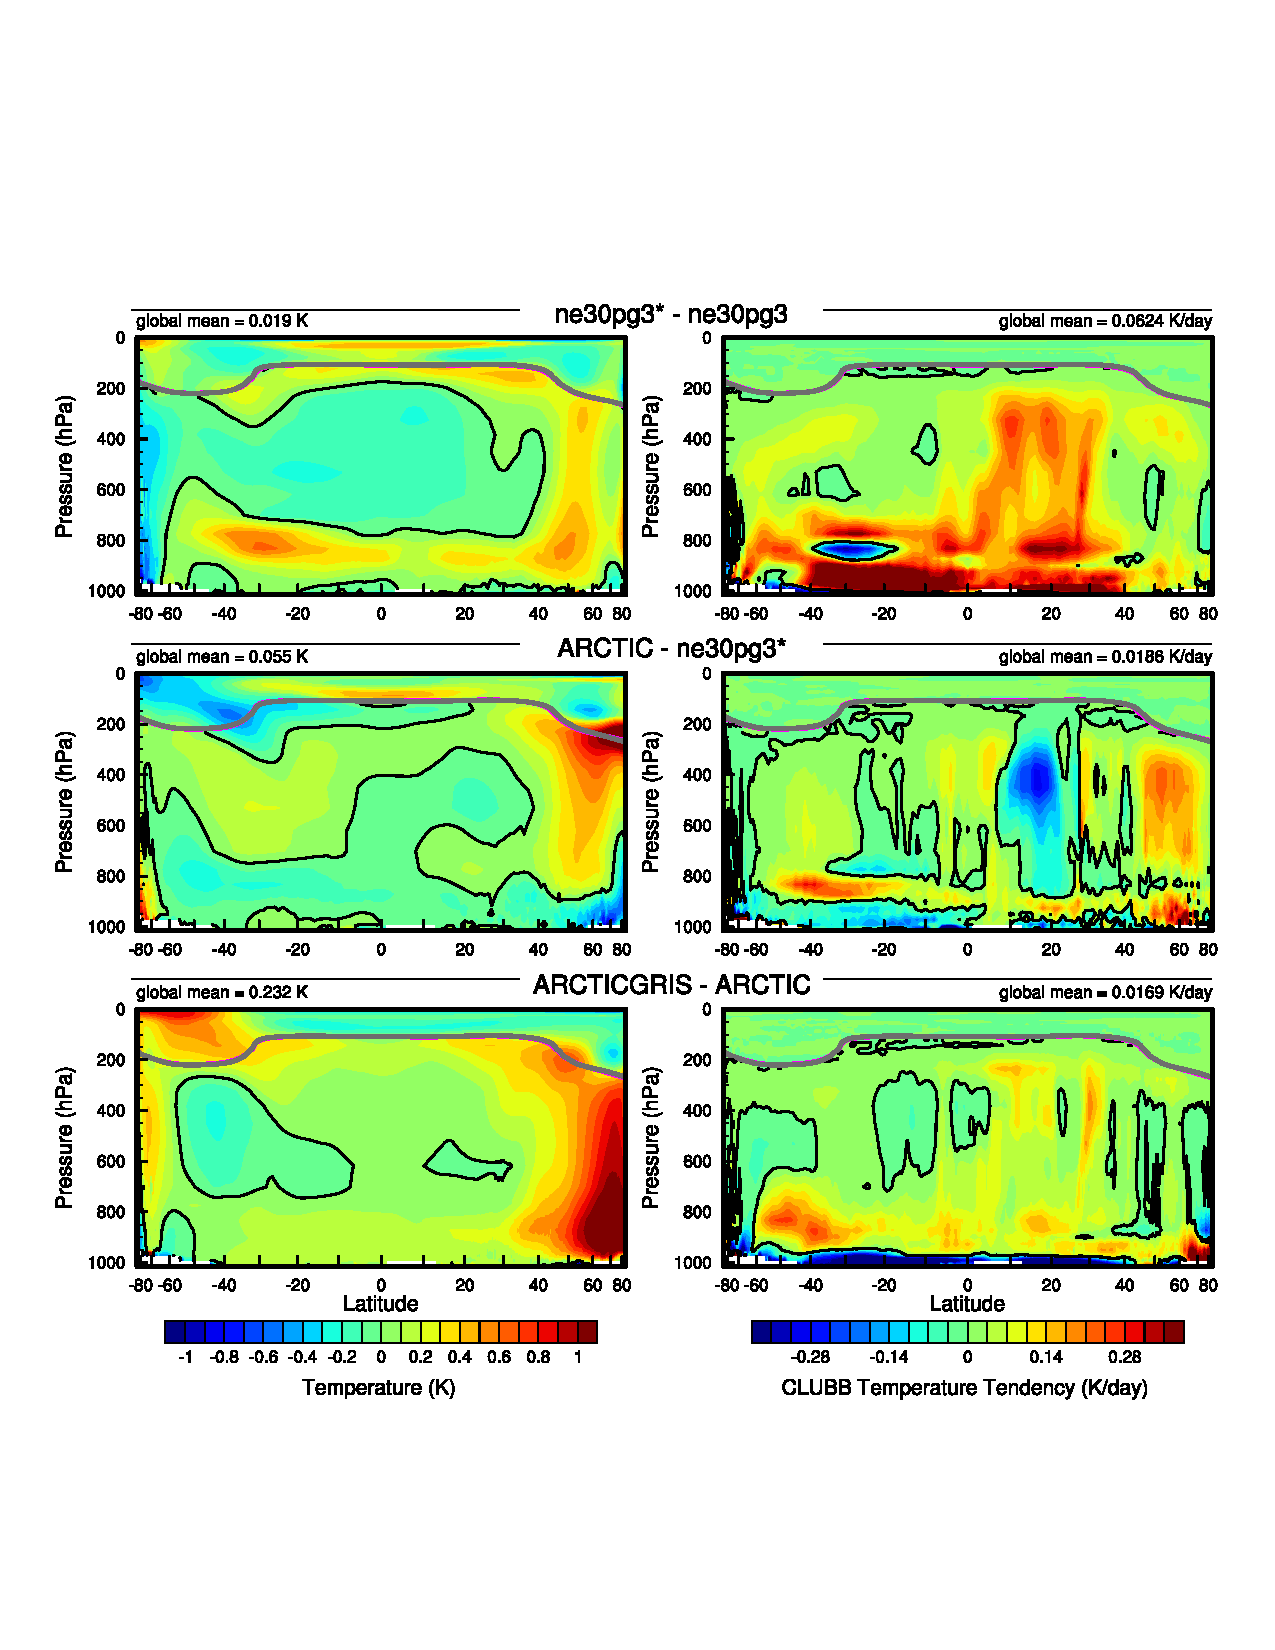
\includegraphics[width=130mm]{figs/temp_dhgt_panel_STEND_CLUBB-hires.pdf}
\end{center}
\caption{As in Figure~\ref{fig:dT-lores} but for the short-time-step experiment and the VR grids. The fields plotted are for the climatological northern hemisphere summer. We focus on summer because that is when the resolution response is largest, and the refined regions are located in the northern hemisphere.}
\label{fig:dT-hires}
\end{figure}

It is useful to understand summer temperature biases due to their control on ice and snow melt over the Greenland Ice Sheet \cite<GrIS;>{O2001JAM}. Figure~\ref{fig:dThyps} shows the 1979--1998 lower troposphere summer temperature bias relative to ERA5. It is computed from the 500--1000 hPa geopotential thickness, solving for the layer-mean virtual temperature using the hypsometric equation ({\color{blue}{Might be good to write this down, for those of us who studied atmospheric science a really long time ago}}). The results are consistent with the zonal mean height plots; increasing resolution from $\tt f19$ to $\tt f09$ warms the climate, and the $1^{\circ}$ SE grids are warmer than the FV grids. The FV summer temperatures are persistently colder than ERA5, whereas the $1^{\circ}$ SE grids are not as cold, and are actually warmer than ERA5 at high-latitudes, north of $75^{\circ}$. All grids show a north-south gradient in bias over Greenland, with the summer temperature bias more positive for the northern part of the ice sheet. This pattern is also evident in the 2m summer temperature bias over Greenland (not shown).

The $\tt Arctic$ grid has summer temperatures similar to the $1^{\circ}$ SE grids, but is slightly warmer over northern Eurasia and the North Pole. An anomalous cooling patch forms to the west of Greenland, centered over Baffin Island. The $\tt Arctic-GrIS$ grid is warmer than the $\tt Arctic$ grid over most of the Arctic, but with a similar spatial pattern of summer temperature bias.

Some of these temperature differences may be related to different summer shortwave cloud forcing for the various grids and dycores. Figure~\ref{fig:SWCF} shows the summer shortwave cloud forcing bias in six runs, using the CERES-EBAF product. 
A negative bias corresponds to excessive reflection and cooling.
The uniform grids have similar biases, with the clouds reflecting 20--40 W/m$^2$ too much shortwave radiation over a wide swath of the Arctic, primarily the land masses ({\color{blue}{please explain what SWCF in caption.}}). There is also a halo of positive bias (clouds not reflective enough) around the ocean perimeter of Greenland. The $\tt Arctic$ grid has much smaller cloud forcing biases over the Arctic land masses, but is still too reflective over Alaska, the Canadian Archipelago, and parts of Eurasia.  Compared to the $\tt Arctic$ grid, the $\tt Arctic-GrIS$ grid vastly reduces the cloud forcing bias over Eurasia, and also improves the bias over North America. In both VR grids, the halo of positive forcing bias around the perimeter of Greenland is absent.

While the summer cloud forcing biases are consistent with the summer temperature biases in Figure~\ref{fig:dThyps} -- regions where clouds are too reflective coincide with regions that are too cold -- it is not clear whether the cold biases are caused by the cloud biases, or whether the cold biases amplify the cloud forcing bias. ({\color{blue}{This ends abruptly. Anything else to add?}} {\color{purple}{Causation I agree is hard to prove due to energy transport, but in summer cloud fraction is probably playing a role. The likely other thing that could be playing a role is surface albedo (absorbed solar). Could note that.}})

\begin{figure}[t]
\begin{center}
         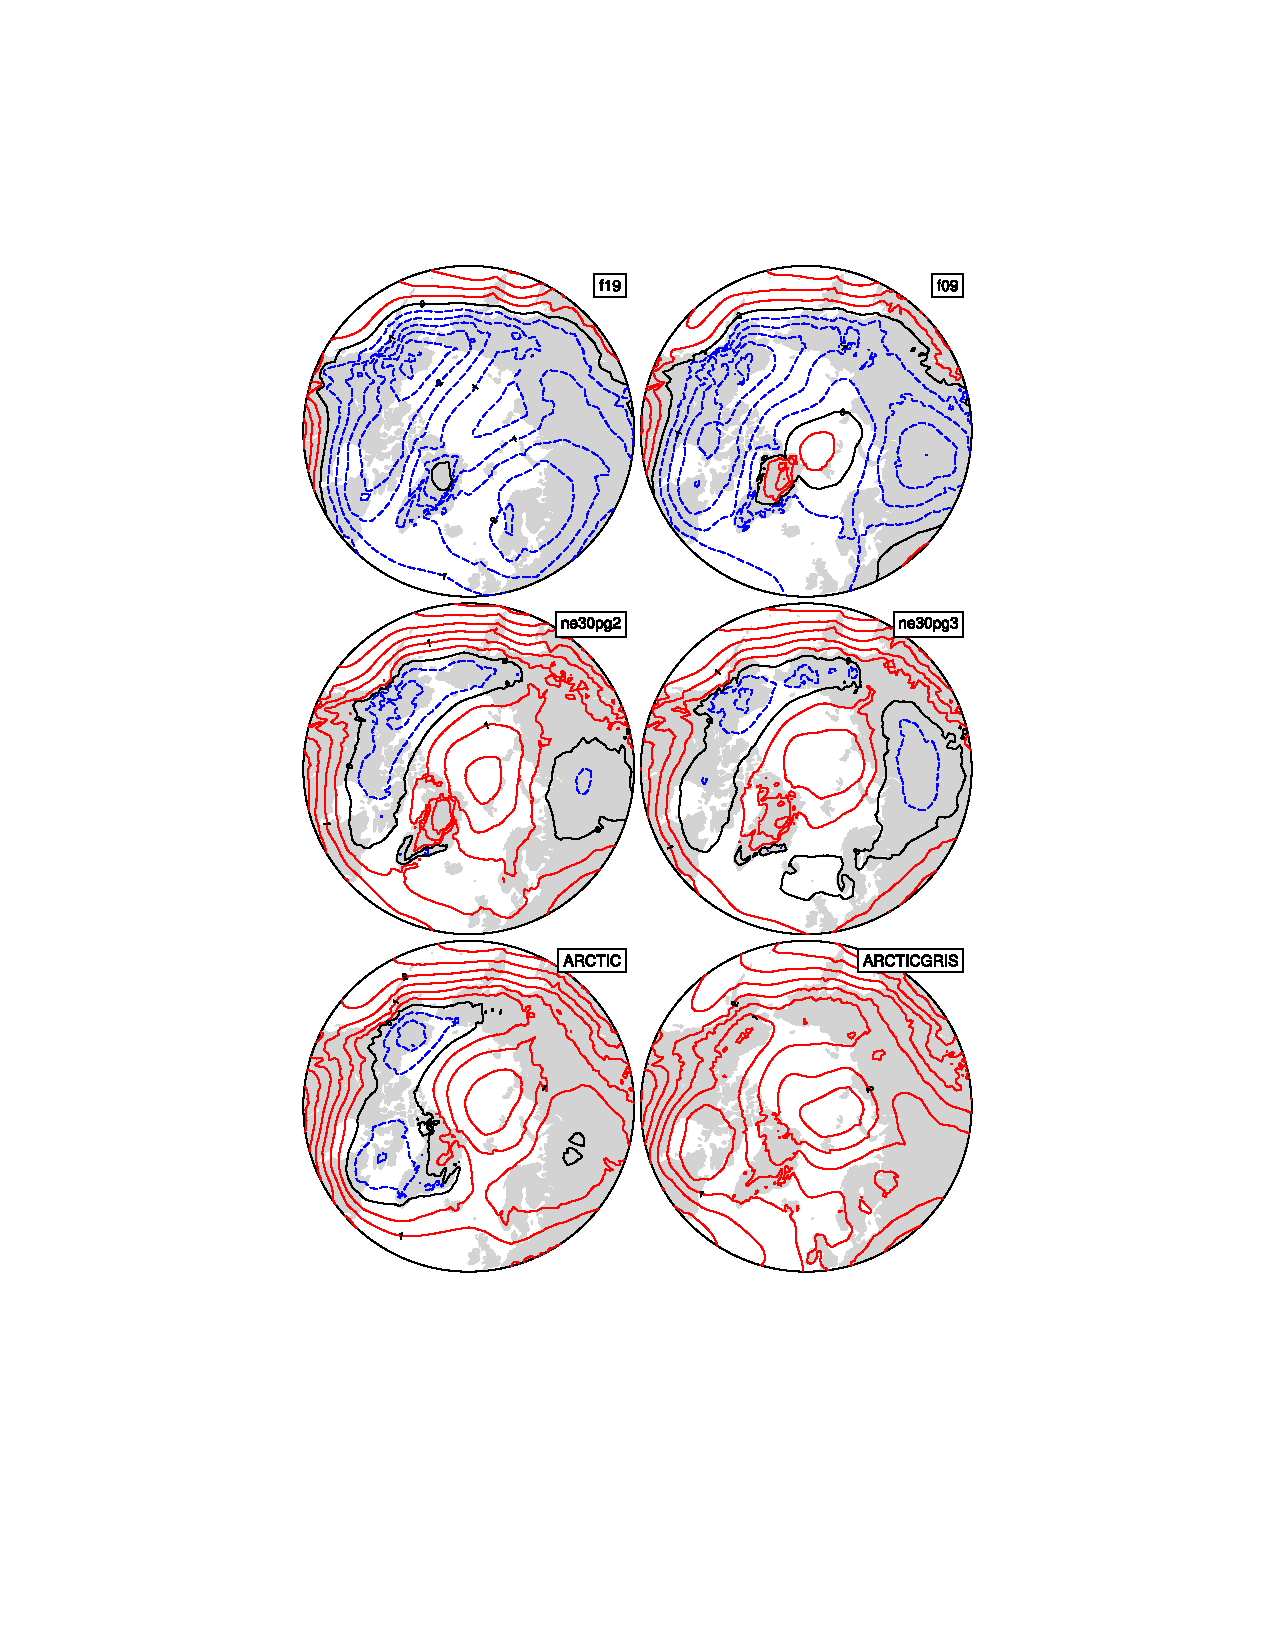
\includegraphics[width=100mm]{figs/temp_contours_diffERA5_Thyps.pdf}
\end{center}
\caption{1979-1998 lower troposphere, northern hemisphere summer virtual temperature biases, computed as the difference from ERA5. Lower troposphere layer mean virtual temperature is derived from the 1000 hPa - 500h Pa geopotential thickness, using the hypsometric equation. Differences are computed after mapping the ERA5 data to the finite-volume grids since the geopotential field is only available on the output tapes in the spectral-element runs that have been interpolated to the $\tt f09$ grid, inline.}
\label{fig:dThyps}
\end{figure}

\begin{figure}[t]
\begin{center}
         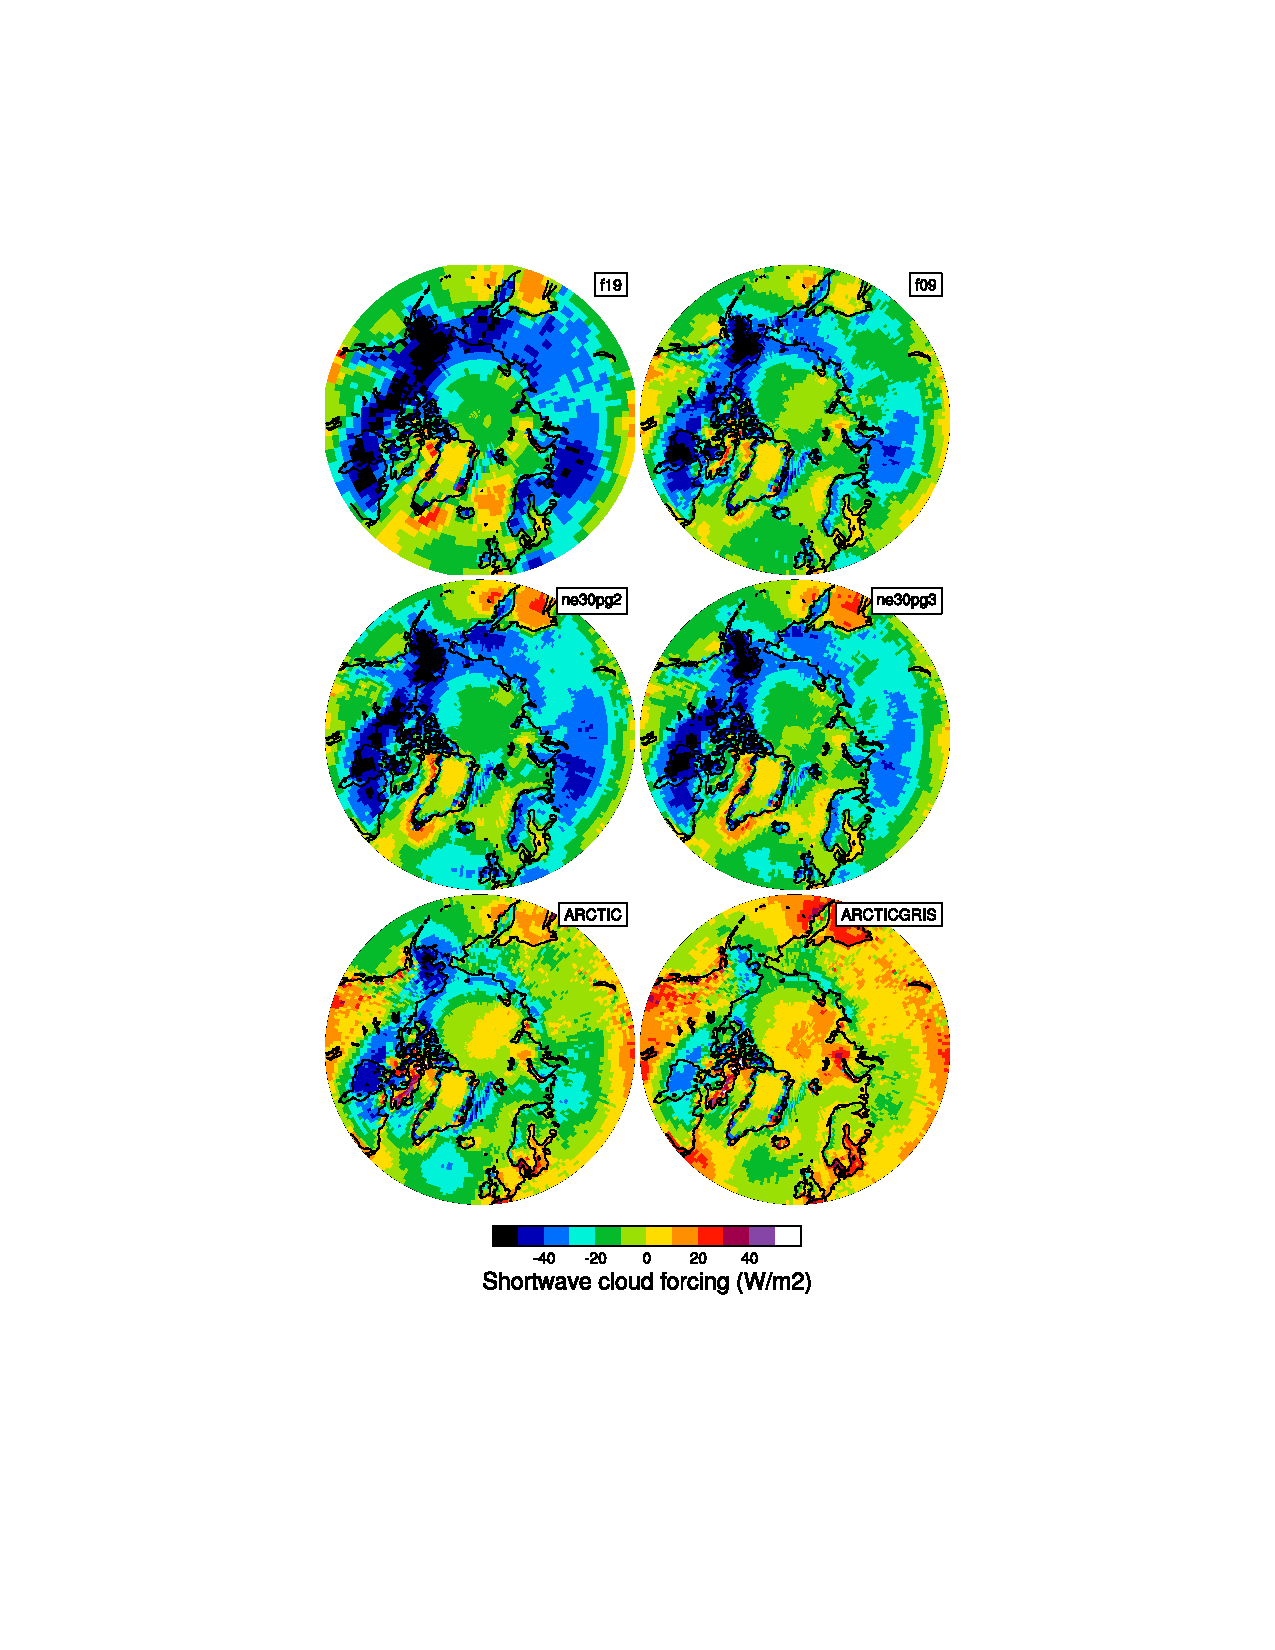
\includegraphics[width=100mm]{figs/temp_contours_diffCERES_SWCF.pdf}
\end{center}
\caption{1979-1998 Northern Hemisphere summer shortwave cloud forcing bias, relative to the CERES-EBAF gridded dataset. Differences are computed after mapping all model output to the $1^{\circ}$ CERES-EBAF grid.}
\label{fig:SWCF}
\end{figure}

\subsection{Shortwave radiation over Greenland}

In addition to summer temperatures, shortwave radiation is an important determinant of snow and ice melt. Figure~\ref{fig:FSDS} shows the summer incident shortwave radiation bias at the surface, zoomed in over Greenland. The top panel shows the bias relative to the CERES-EBAF dataset, and the bottom panel relative to the RACMO2.3p2 dataset.
The halo of excessive incident shortwave radiation around the coasts of Greenland is apparent for both datasets in relation to the coarser grids, consistent with the shortwave cloud forcing biases in Figure~\ref{fig:SWCF}.

The ice sheet interior receives too little shortwave radiation on the coarser grids. On the VR grids, both the interior shortwave deficit and the excessive shortwave around the ocean perimeter are improved. This suggests that the coarse-grid clouds are too thick in the Greenland interior and too thin around the perimeter, and that increasing horizontal resolution reduces these biases. This is consistent with the total summer cloud fraction bias, computed from the CALIPSO-GOCCP cloud dataset  and shown in Figure~\ref{fig:prect}. Note that total cloud fraction characterizes the cloud field at all vertical levels, but attenuates the changes arising from any single layer due to the maximum overlap assumption used to compute this quantity. Despite the attenuated signal, the total cloud fraction for the VR grids does indicate reduced cloud coverage in the interior and increased cloudiness around the ocean perimeter. 

The agreement of the cloud biases in and around Greenland from multiple independent datasets shows that the biases are a robust feature of the coarser grids. The reduced biases on the VR grids suggest that the coarse-grid biases are a result of insufficient horizontal resolution.

\begin{figure}[t]
\begin{center}
         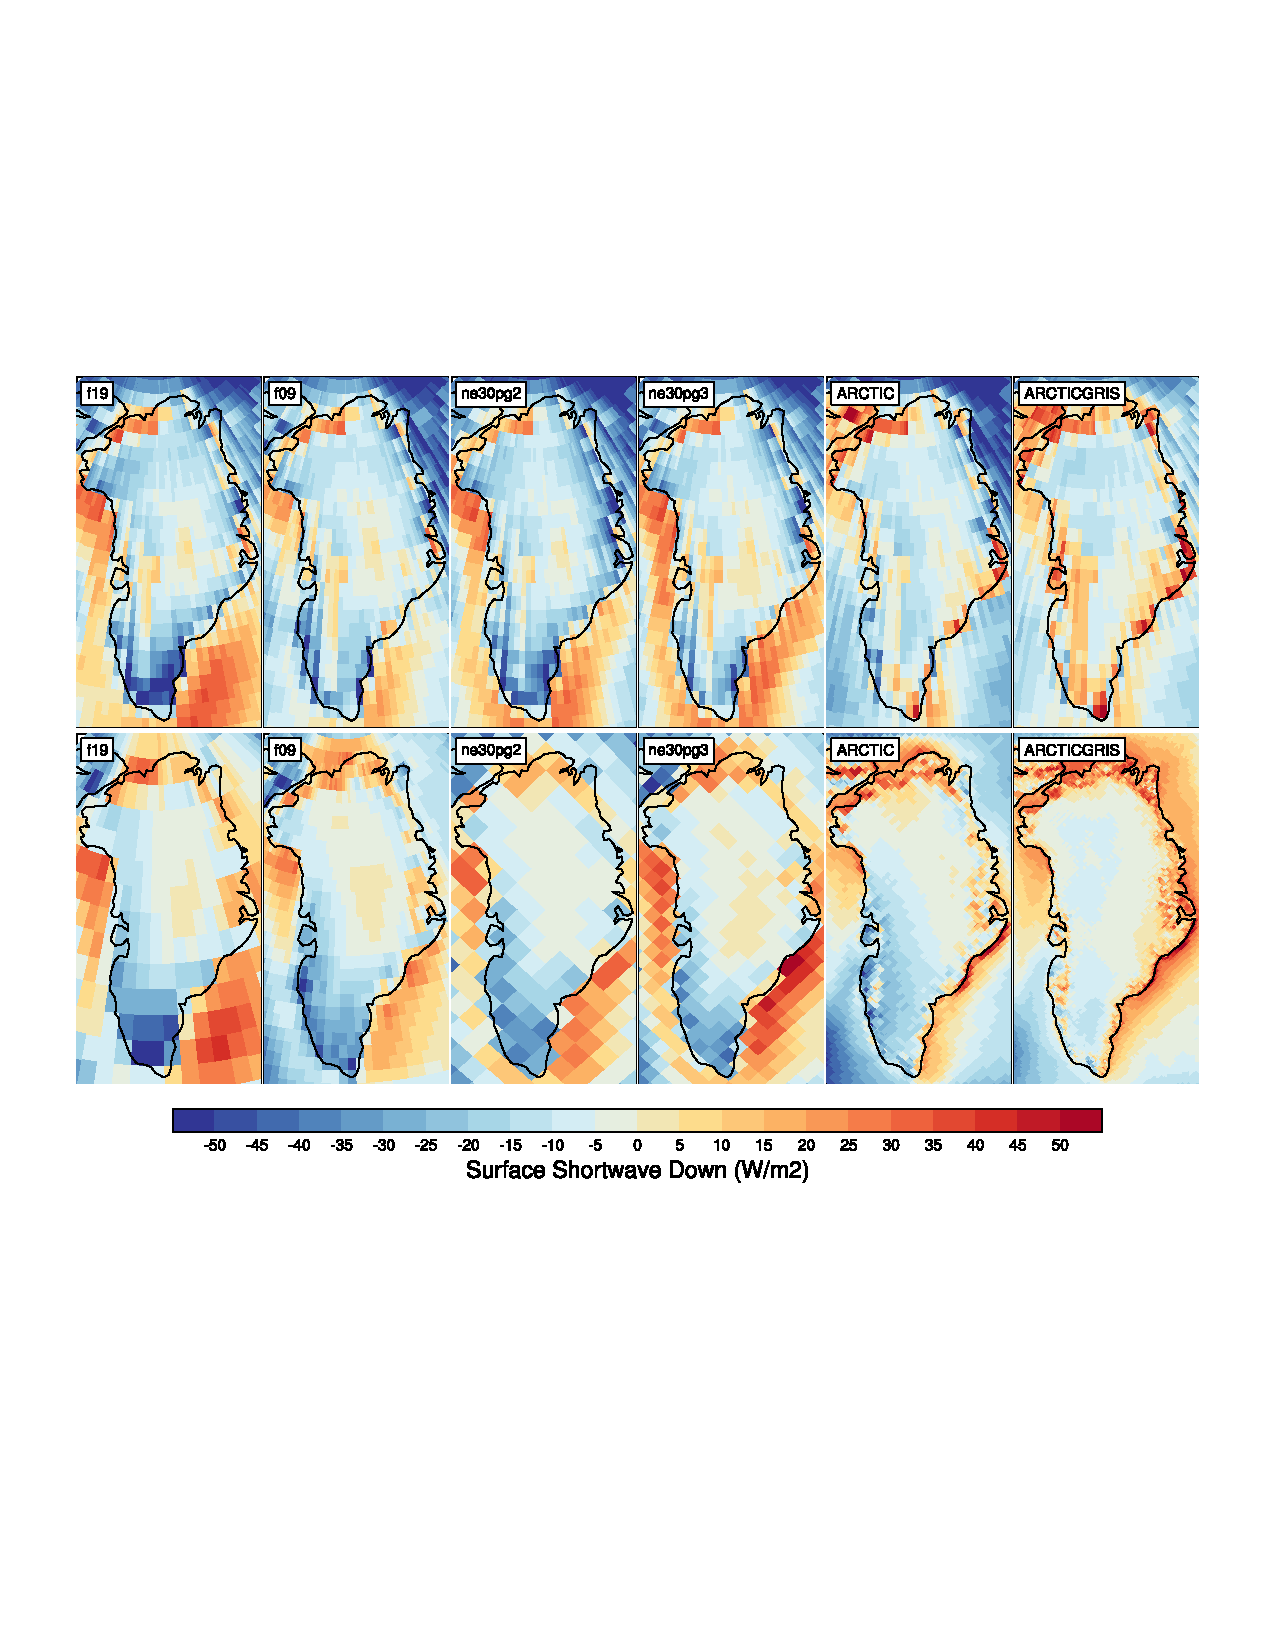
\includegraphics[width=130mm]{figs/temp_contours_diffCERESdiffRACMO_FSDS.pdf}
\end{center}
\caption{1979-1998 northern hemisphere summer, incident shortwave radiation bias, computed as the difference (top) from CERES-EBAF, and (bottom) RACMO2.3p2 dataset. The differences in the top panel are found by mapping the model output to the $1^{\circ}$ CERES-EBAF grid, and differences on the bottom panel are computed after mapping the RACMO2.3p2 dataset to the individual model grids. Note that the averaging period for the CERES-EBAF panels, 2003-2020, is different from the averaging period for the model results.}
\label{fig:FSDS}
\end{figure}

\begin{figure}[t]
\begin{center}
         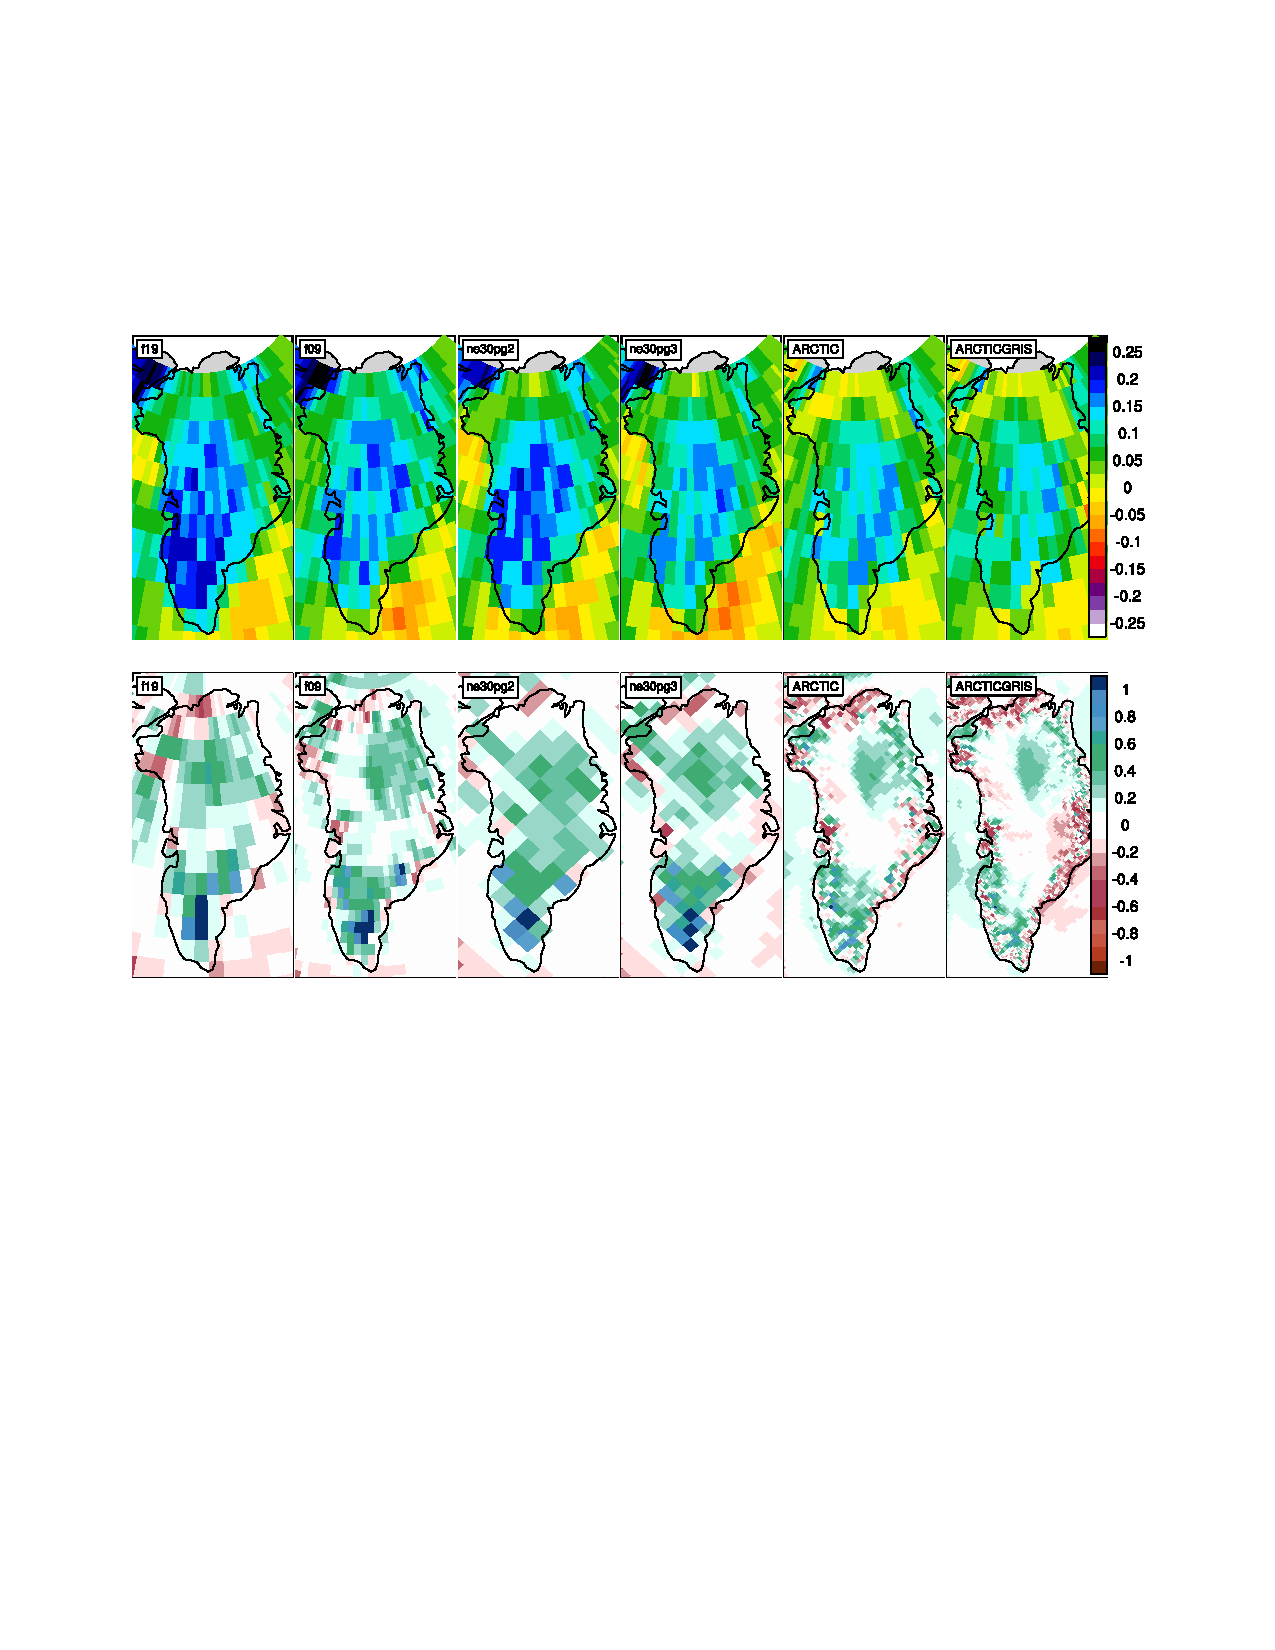
\includegraphics[width=130mm]{figs/temp_contours_diffCERESdiffRACMO_CLOUD_PRECIP.pdf}
\end{center}
\caption{1979-1998 northern hemisphere summer (top) total cloud fraction bias, relative to the CALIPSO-GOCCP dataset, and (bottom) precipitation rate bias, relative to the RACMO2.3p2 dataset. The CALIPSO-GOCCP differences are computed after mapping all model output to the $1^{\circ}$ grid, whereas the RACMO differences are computed after mapping the RACMO dataset to the individual model grids. Note that the averaging period for the CALIPSO-GOCCP panels (2006-2017) is different than the model averaging period. \color{red}{ARH - still trying to fix the layout of this figure so the label bars aren't on top of the panels}.}
\label{fig:prect}
\end{figure}

\subsection{Greenland surface mass balance}

The accuracy of the simulated SMB is expected to be sensitive to grid resolution. Figure~\ref{fig:gridsdx}b shows the average grid spacing over the Greenland Ice Sheet (GrIS) in all six grids in this study. The $\tt ne30pg2$ grid has the coarsest representation with an average $\Delta x=160~km$, and the $\tt Arctic-GrIS$ grid has the highest resolution with an average $\Delta x=14.6~km$, similar to the grid spacing of the $11~km$ RACMO2.3 grid. The $\tt ne30pg3$ grid has an average $\Delta x=111.2~km$, substantially coarser than the $\tt f09$ grid, with an average $\Delta x=60~km$. Although $\tt ne30pg3$ and $\tt f09$ have similar average grid spacing over the entire globe, and comparable computational costs, the convergence of meridians on the FV grid enhances the resolution over the GrIS. The $\tt Arctic$ grid has an average grid spacing of $\Delta x=27.8~km$, and is about 10 times more expensive than the $1^{\circ}$ models.  The $\tt Arctic-GrIS$ grid is about twice as expensive as the $\tt Arctic$ grid. ({\color{blue}{Wondering if this paragraph would go better in an earlier section. Rene agrees}})

The lower panels of Figure~\ref{fig:prect} show the summer climatological mean precipitation bias over the GrIS, expressed as the fractional difference from the RACMO2.3p2 solution. The coarse $1^{\circ}-2^{\circ}$ grids have large, positive biases centered over the southern dome. The $\tt Arctic$ grid reduces this bias substantially, and the $\tt Arctic-GrIS$ grid reduces it further. This suggests that the southern dome bias arises from inadequate horizontal resolution, consistent with the original GrIS VR experiments in \citeA{VETAL2018TC}. 

Large GrIS accumulation rates result from synoptic systems arriving from the south. These systems are orographically lifted at the ice sheet margin, especially over the steep slopes in southeast Greenland, concentrating heavy precipitation near the ice margin. At lower resolutions, the topography is too smooth and moisture penetrates inland, erroneously dumping precipitation onto the southern dome. The ability of the VR grids to more accurately simulate orographic precipitation is consistent with the cloud results above. As the precipitation centers move from the interior toward the margins, and even out over the ocean with increasing resolution, the cloud decks move accordingly. Figures~\ref{fig:SWCF}, \ref{fig:FSDS}, and \ref{fig:prect} clearly illustrate a shift in clouds from the interior to the ocean perimeter with increasing resolution.

 \begin{table*}
 \centering
 \scriptsize
 \begin{tabular}{lccccc}
   \hline
   grid name & accumulation & total melt & runoff & sublimation & SMB \\ 
   \hline
   $RACMO$ & 768.5 (733.5) & -347.2 (-436.4) & -221.7 (-258.5) & -36.5 (-38.8) & 510.3 (436.2) \\
   \hline
   $\tt f19$ & 882.5 (913.5) & -440.3 (-546.5) & -283.7 (-284.3) & -36.6 (-37.5) & 562.2 (591.7) \\
   $\tt f09$ & 874.8 (882.1) & -418.4 (-482.3) & -255.0 (-212.3) & -38.1 (-37.4) & 581.7 (632.4) \\
   $\tt ne30pg2$ & 1000. (973.4) & -549.4 (-647.3) & -383.9 (-347.0) & -33.4 (-32.1) & 582.7 (594.3) \\
   $\tt ne30pg3$ & 934.9 (909.3) & -568.8 (-686.7) & -356.2 (-330.1) & -34.4 (-32.6) & 544.3 (546.6) \\
   $\tt Arctic$ & 795.9 (818.6) & -367.3 (-436.8) & -208.9 (-194.2) & -44.1 (-43.9) & 542.9 (580.5) \\
   $\tt Arctic-GrIS$ & 708.7 (747.3) & -471.6 (-610.4) & -261.1 (-307.8) & -50.7 (-51.8) & 396.9 (387.7) \\
 \hline
 \end{tabular}
  \caption{1979-1998 surface mass balance of the Greenland Ice Sheet in Gt/yr. Values shown are using the common ice mask approach described in the methods section, whereas values in parentheses are from integrating over the native grid and ice mask. {\color{red}{ARH - these numbers need updating ... they are only for method 1.}}}
 \label{tbl:table3}
 \end{table*}

\begin{figure}[t]
\begin{center}
         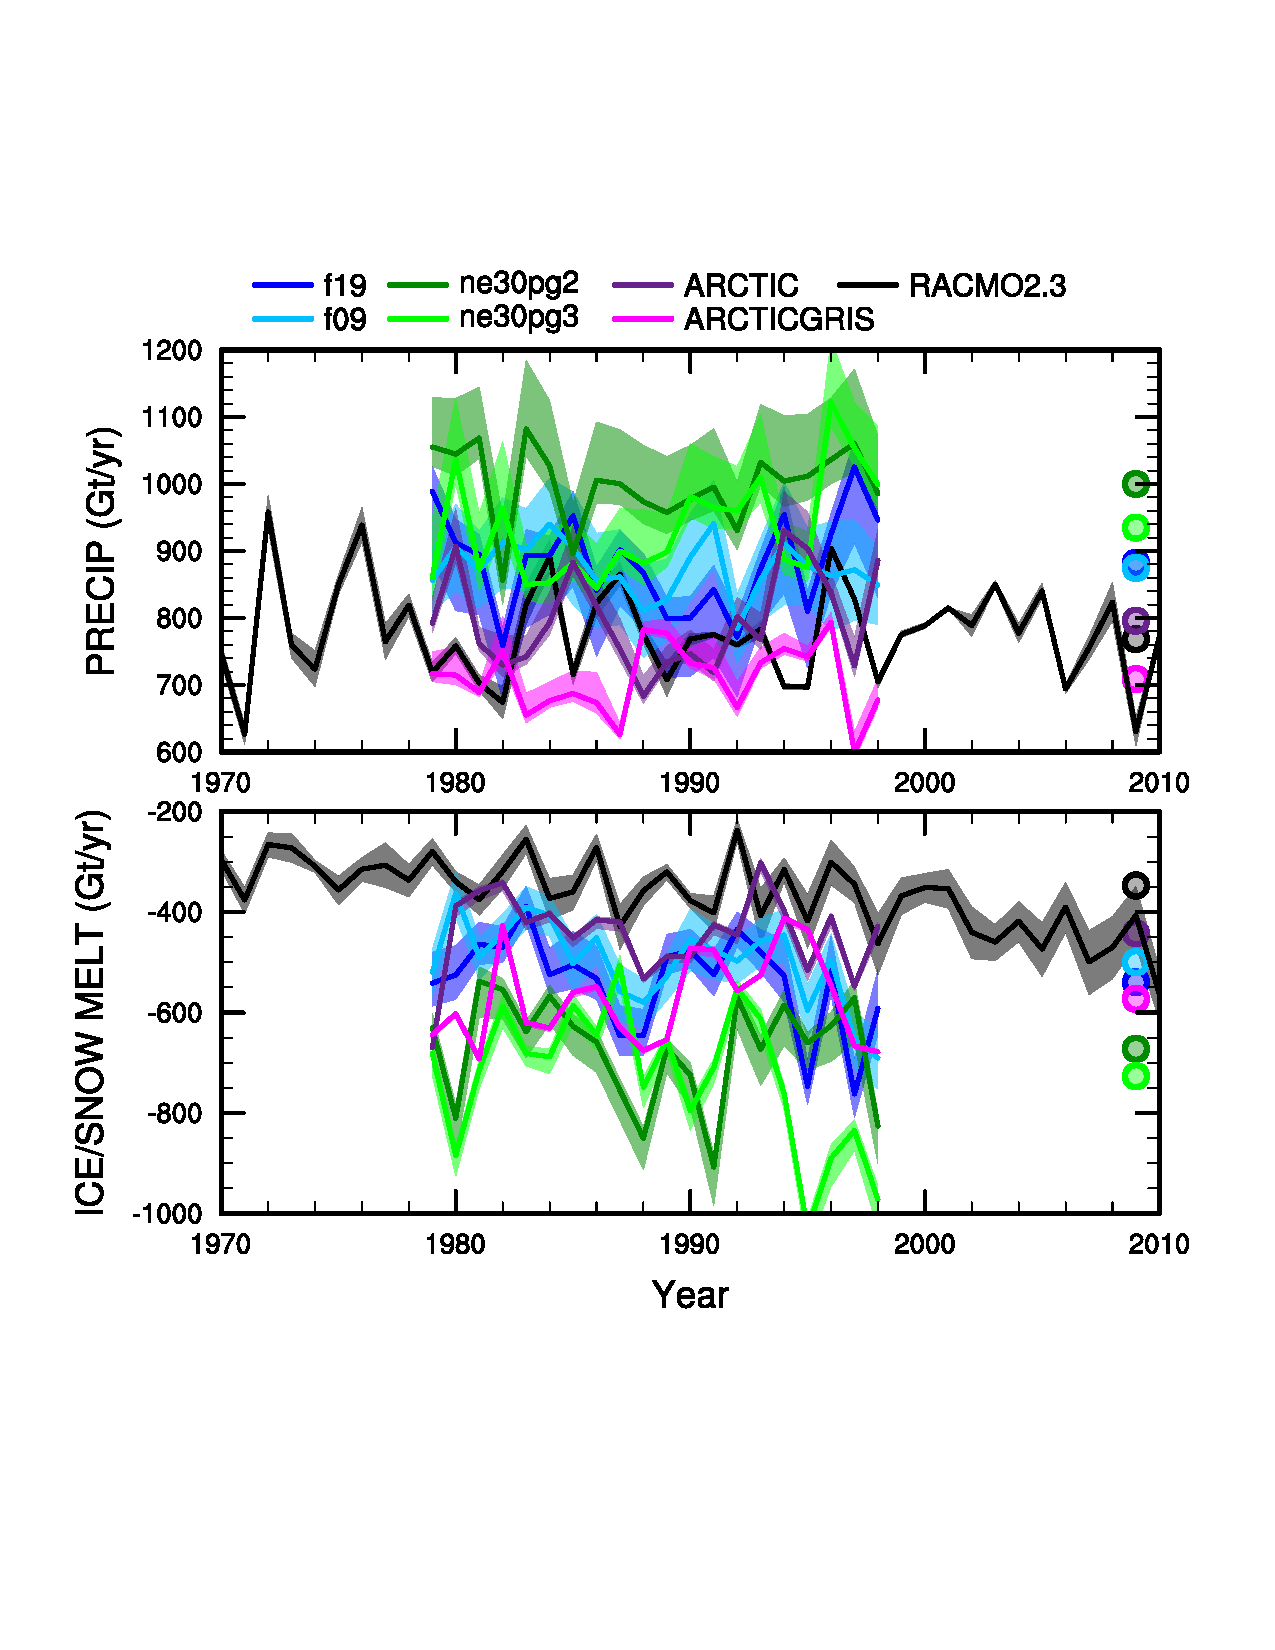
\includegraphics[width=100mm]{figs/temp_tseries_GRIS.pdf}
\end{center}
\caption{Time-series of annual (solid+liquid) precipitation (top) and annual runoff (bottom) integrated over the Greenland Ice Sheet for all six simulations and compared to the RACMO datasets. The time-series were generated using the common ice mask approach, which results in up to 4 ensembles, with the mean value given by the solid line and shading spanning the extent of the ensemble members.}
\label{fig:tseries}
\end{figure}

Table~\ref{tbl:table3} shows the 1979-1998 climatological SMB components for each grid, compared with RACMO {\color{purple}{Andrew - do you want to talk about the values at all?}}.
The CESM values are averages over the ensemble of common ice masks and regridding methods described in section~\ref{sec:SMB}, and the RACMO values are averages over both RACMO datasets (Table~\ref{tbl:table2}) using the same common-ice-mask approach. Table~\ref{tbl:table3} also contains (in parentheses) the SMB components derived from evaluating the integrals on each model's native grid and ice mask. Of note is the large reduction in melt rates using the common-ice-mask approach compared to the native grid, illustrating the dissipation discussed in section~\ref{sec:SMB}. The errors are greatest in partially ice-covered grid cells straddling the ice sheet margins, in the ablation zone where melt rate are large. For integrated precipitation, the differences between the native and common-ice-mask approaches are much smaller, since the combined solid/liquid precipitation rates are not directly tied to the ice mask.

Figure~\ref{fig:tseries} shows time series of annually integrated precipitation and snow/ice melt over the GrIS for the various different grids and dycores, with both versions of RACMO shown in black. The 1979-1998 climatological mean values, listed in Table~\ref{tbl:table3}, are shown as circles on the right side of the panels. The uniform $1^{\circ}-2^{\circ}$ grids have positive precipitation biases in the interior, whereas the VR grids have the smallest biases, with precipitation comparable to RACMO. The $\tt f19$ and $\tt f09$ grids perform similarly, with +110 Gt/yr bias, whereas $\tt ne30pg3$ is biased by about +165 Gt/yr and $\tt ne30pg2$ by +230 Gt/yr. The larger biases on the uniform-resolution SE grids relative to the FV grids are consistent with the coarser GrIS resolution on the SE grids (Figure~\ref{fig:grisdx}).

The combined annual snow/ice melt shown in the bottom panel of Figure~\ref{fig:tseries} indicates that the $\tt Arctic$ grid simulates the most realistic melt rates, with the other grids having more melt than RACMO. The $\tt Arctic-GrIS$ grid overpredicts melting by about 125 Gt/yr. This is likely due to an anomalously warm lower troposphere during the summer, relative to the $\tt Arctic$ run (Figure~\ref{fig:dThyps}). The $\tt f19$ and $\tt f09$ melting rates are improved over $\tt Arctic-GrIS$, overestimating melt by only 70--90 Gt/yr. The SE grids have the largest positive melt bias, between 200--220 Gt/yr. It is more difficult to attribute these differences to resolution alone, since the FV grids have colder summer temperatures than the uniform-resolution SE grids. ({\color{blue}{Not sure I understand this sentence.  FV is both cooler and higher-resolution than SE, so one might suspect that cooler T is, in fact, connected to higher resolution.}})

To illustrate the regional behavior of the SMB components, Figure~\ref{fig:basin} shows the precipitation and combined snow/ice melt integrated over the basins defined by \citeA{RM2012GRL}. The uncertainty due to differences in basin area is larger than for GrIS-wide integrals, owing to the differences in basin boundaries as represented by the common ice masks, which are shown in the $\tt f19$ and $\tt ne30pg2$ panels of Figure~\ref{fig:melt}. Nonetheless, the regional totals in Figure~\ref{fig:basin} correctly show the southeast and southwest basins have the most accumulation. In all basins, accumulations drops monotonically with increasing grid resolution, with some exceptions. The $\tt Arctic-GrIS$ grid simulates less precipitation than RACMO in the central-east and southeast basins, and is closest of all grids to the RACMO precipitation in the large southwest basin.

\begin{figure}[t]
\begin{center}
         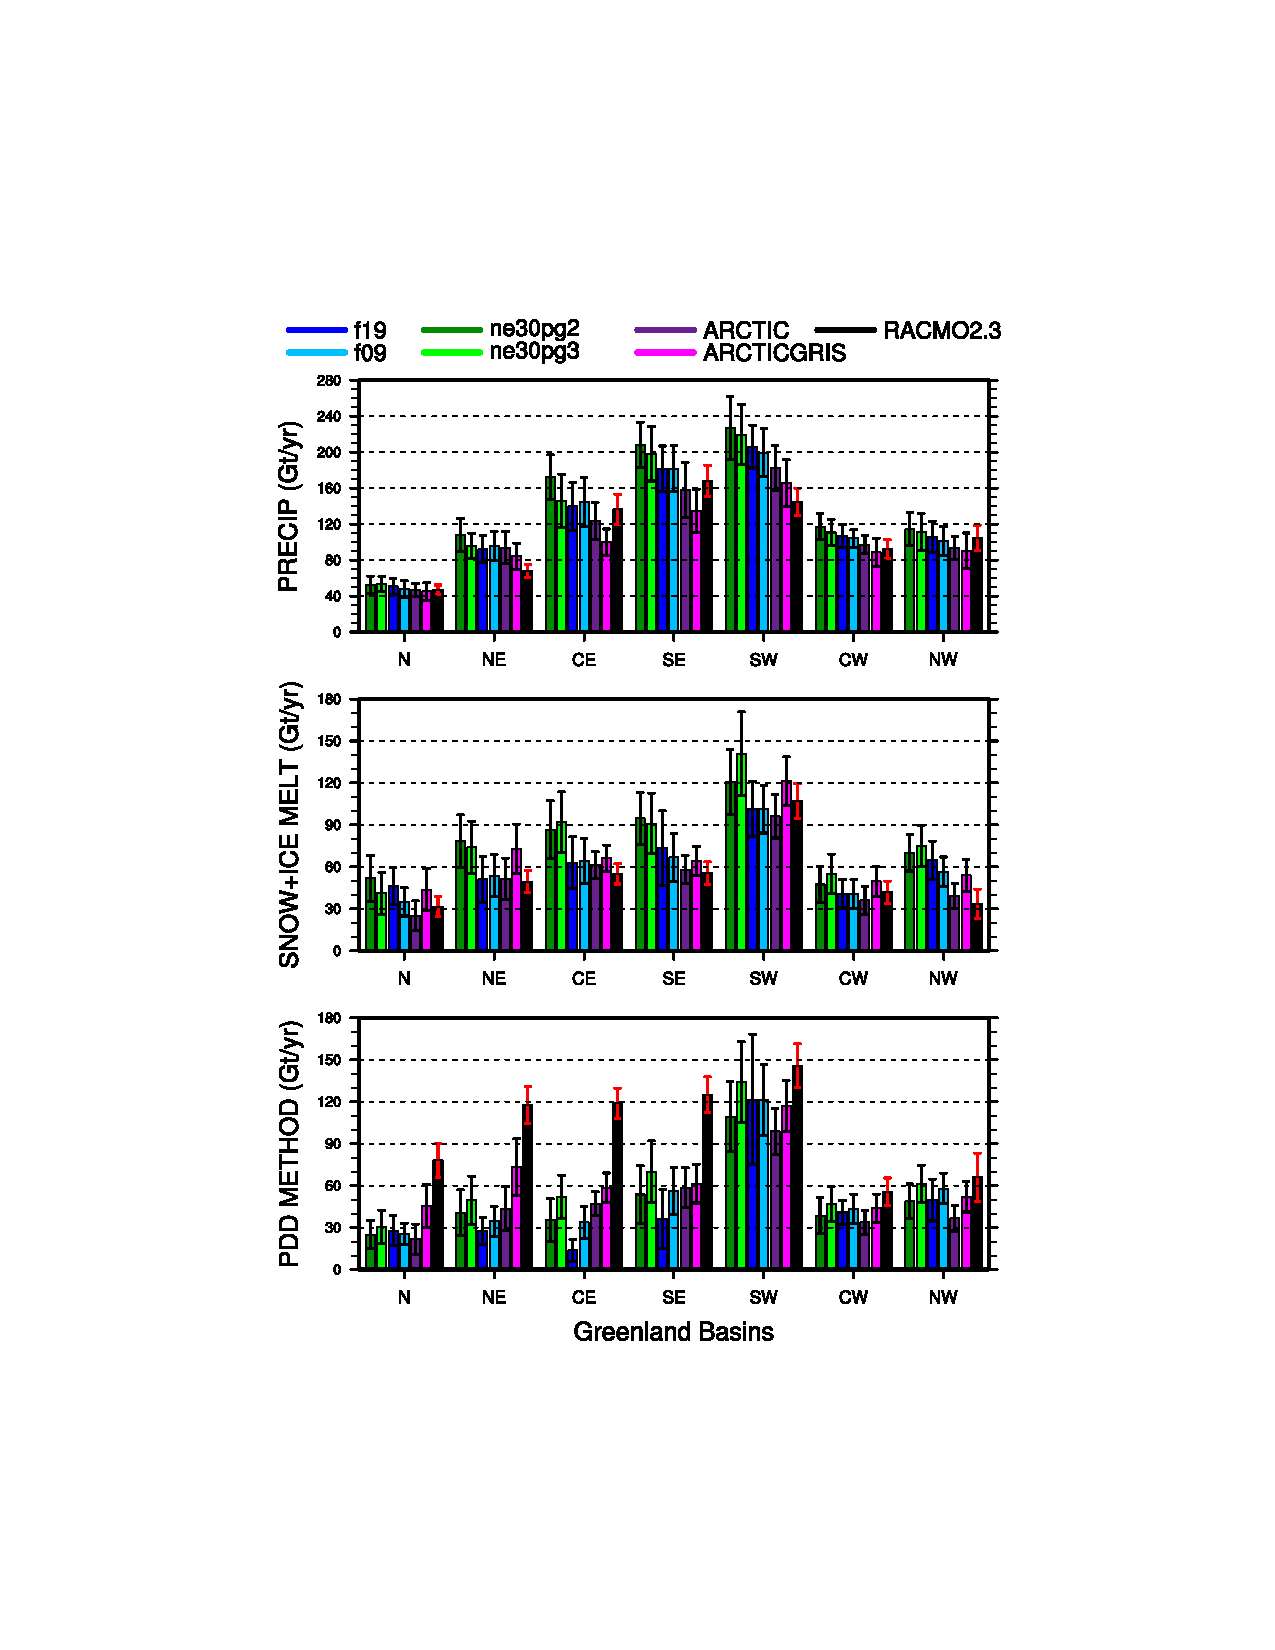
\includegraphics[width=100mm]{figs/temp_tseries_BASIN.pdf}
\end{center}
\caption{1979--1998 basin integrated components of the SMB; (top) precipitation, (middle) ice/snow melt and (bottom) ice/snow melt estimated from the PDD method. Whiskers span the max/min of the four ensemble members generated from the common-ice-mask approach. Basin definitions are after \citeA{RM2012GRL}, and are found on the common ice masks using a nearest neighbor approach, and shown in Figure~\ref{fig:melt}.}
\label{fig:basin}
\end{figure}

\begin{figure}[t]
\begin{center}
         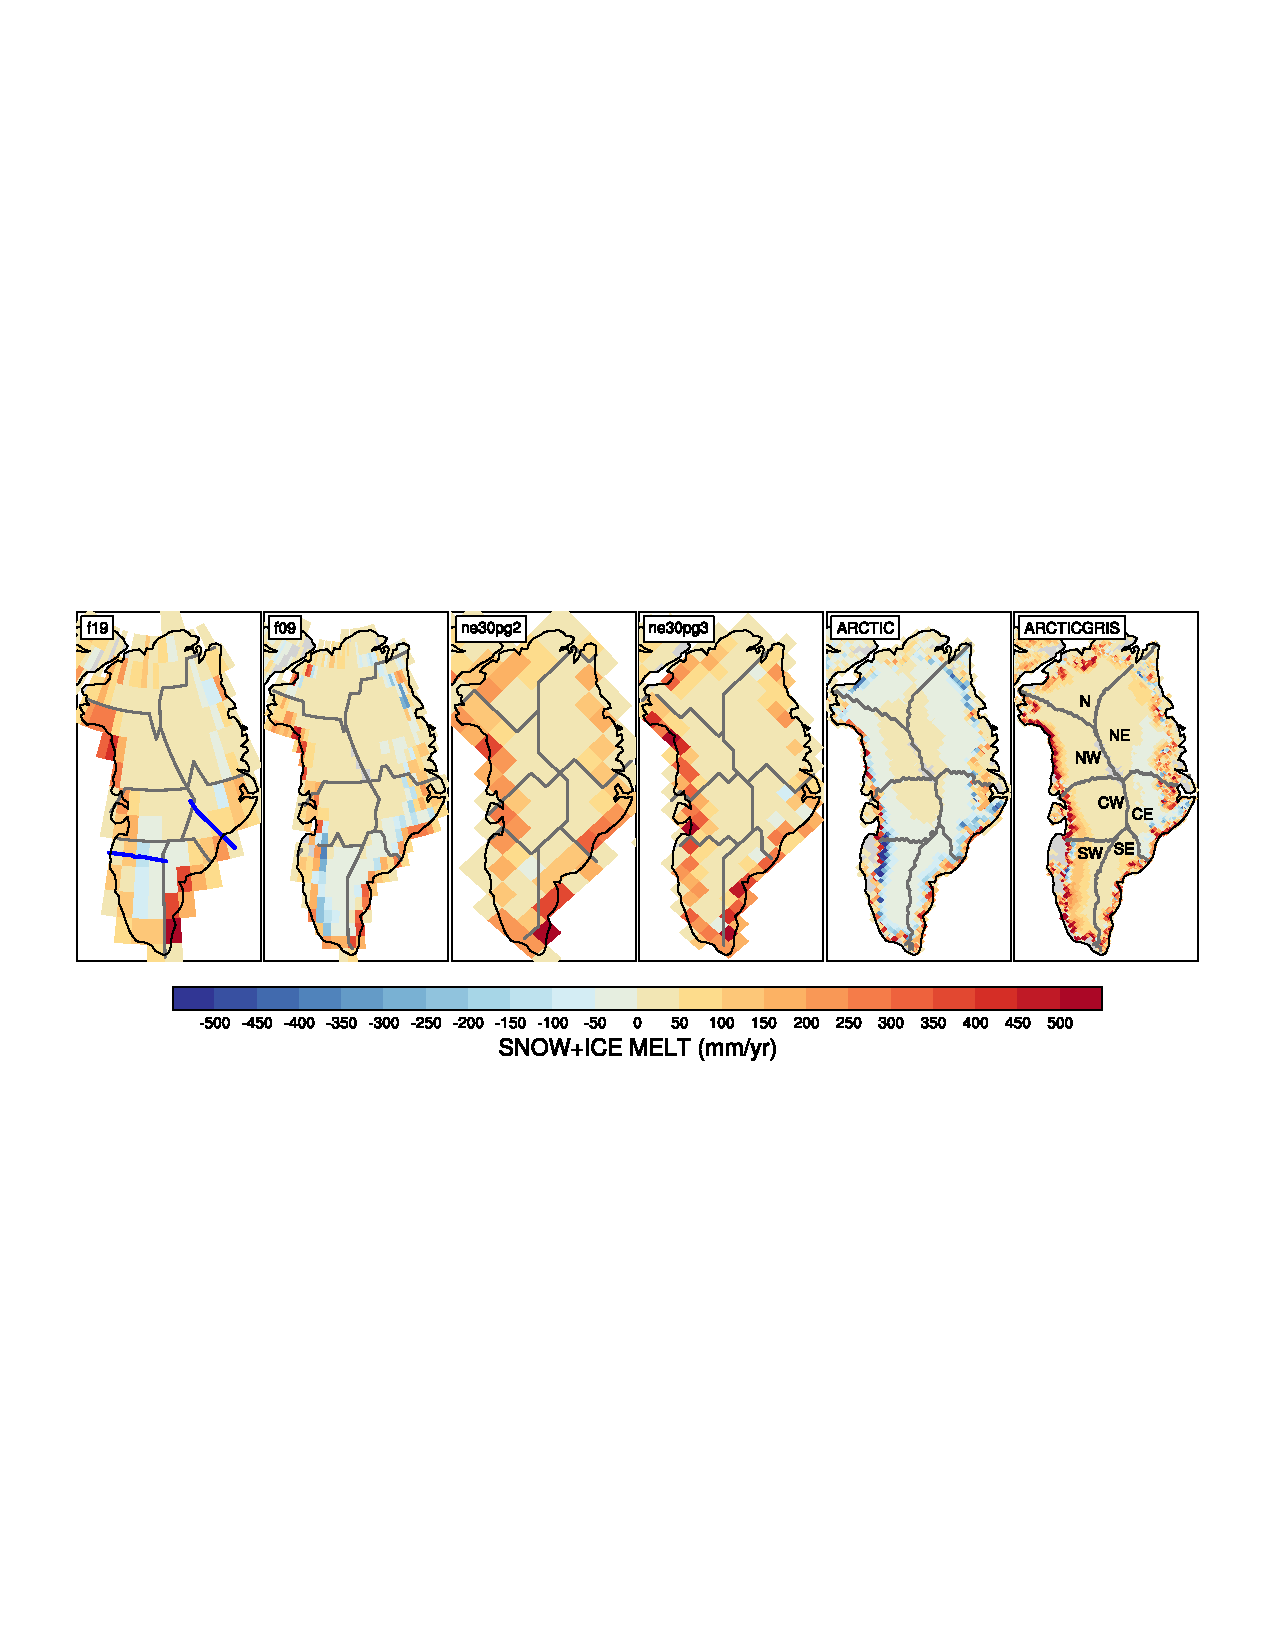
\includegraphics[width=130mm]{figs/temp_contours_diffRACMO_melt.pdf}
\end{center}
\caption{1979--1998 ice/snow melt biases (in mm/yr) relative to RACMO2.3p2, evaluated on the native model grids. The \citeA{RM2012GRL} basin boundaries are shown in grey for each model grid. Note that Figure~\ref{fig:basin} uses the basin boundaries for the two common ice masks, shown in the $\tt f19$ and $\tt ne30pg2$ panels, in computing the basin-scale integrals. Blue lines in the $\tt f19$ panel show the location of the two transects plotted in Figure~\ref{fig:ztrans}.}
\label{fig:melt}
\end{figure}

The basin-integrated melt rates in Figure~\ref{fig:basin} depend on the dycore. The uniform-resolution SE grids have the largest positive biases in all basins. The $\tt Arctic-GrIS$ grid is a close second, while the FV grids have systematically smaller melt-rates. The ``second-place" standing of $\tt Arctic-GrIS$ is somewhat unexpected, as this grid has the warmest lower-troposphere summer temperatures (Figure~\ref{fig:dThyps}) and greatest incident shortwave radiation (Figure~\ref{fig:FSDS}), yet it has less melting than the uniform-resolution SE grids.

Lower troposphere temperature is not a strict proxy for melting; e.g., it may not capture microclimate effects as a result of a better representation of the low-elevation ablation zones. Positive degree-days \cite<PDD;>{B1984Z}, which accumulate the near-surface temperature in $^{\circ}C$ for days with temperature above freezing, are a more accurate proxy.
PDD is nonlinear in mean monthly temperature \cite{R1991P}.  We compute it from monthly mean 2-meter temperature using the method of \citeA{CG2005JG}, assuming a fixed monthly mean standard deviation of 3$^{\circ}$C and a degree-day factor of 5~mm~d$^{-1}$ $^{\circ}$C$^{-1}$.

Figure~\ref{fig:basin}c shows the basin-integrated PDD melt estimate.  In the large southeast and southwest basins (and all the other western basins), the $\tt ne30pg3$ grid has larger PDD-based melt than the $ARCTCGRIS$ grid. The FV grids also have large PDD-based melt in the southwest basin, relative to $\tt Arctic-GrIS$. The PDD plots indicate that the near-surface temperatures which contribute to melt are not well approximated by the summer lower-troposphere temperatures in Figure~\ref{fig:dThyps}.

Figure~\ref{fig:melt} presents the biases in the combined ice/snow melt as map plots. These plots show that the largest melt biases are on the southeast and northwest coasts, where large coarse-grid cells overlap with the ocean. One possibility is that these problematic grid cells are situated at lower elevations than the true ice sheet surface, leading to a warm bias and too much melt. Figure~\ref{fig:ztrans} shows the representation of the ice sheet surface along two transects on the different grids, compared to the high-resolution dataset used to generate CAM topographic boundary conditions \cite{GMTED2010,gmdd-8-4623-2015}. The two transects are shown in Figure~\ref{fig:melt}: the east-west ``K-transect'' in southwest Greenland and a transect extending from the central dome down to the  Kangerlussuaq glacier on the southeast coast. The $1^{\circ}-2^{\circ}$ grids are noticeably coarse, with only a few grid cells populating the transect. The $\tt f09$ grid is a bit of an exception for the K-transect, with grid cells becoming narrow in the meridional direction at high latitudes. The VR grids are more skillful at reproducing the steep margins of the ice sheet, capturing the parabolic shape of the GrIS margins.

\begin{figure}[t]
\begin{center}
\begin{tabular}{cccc}
         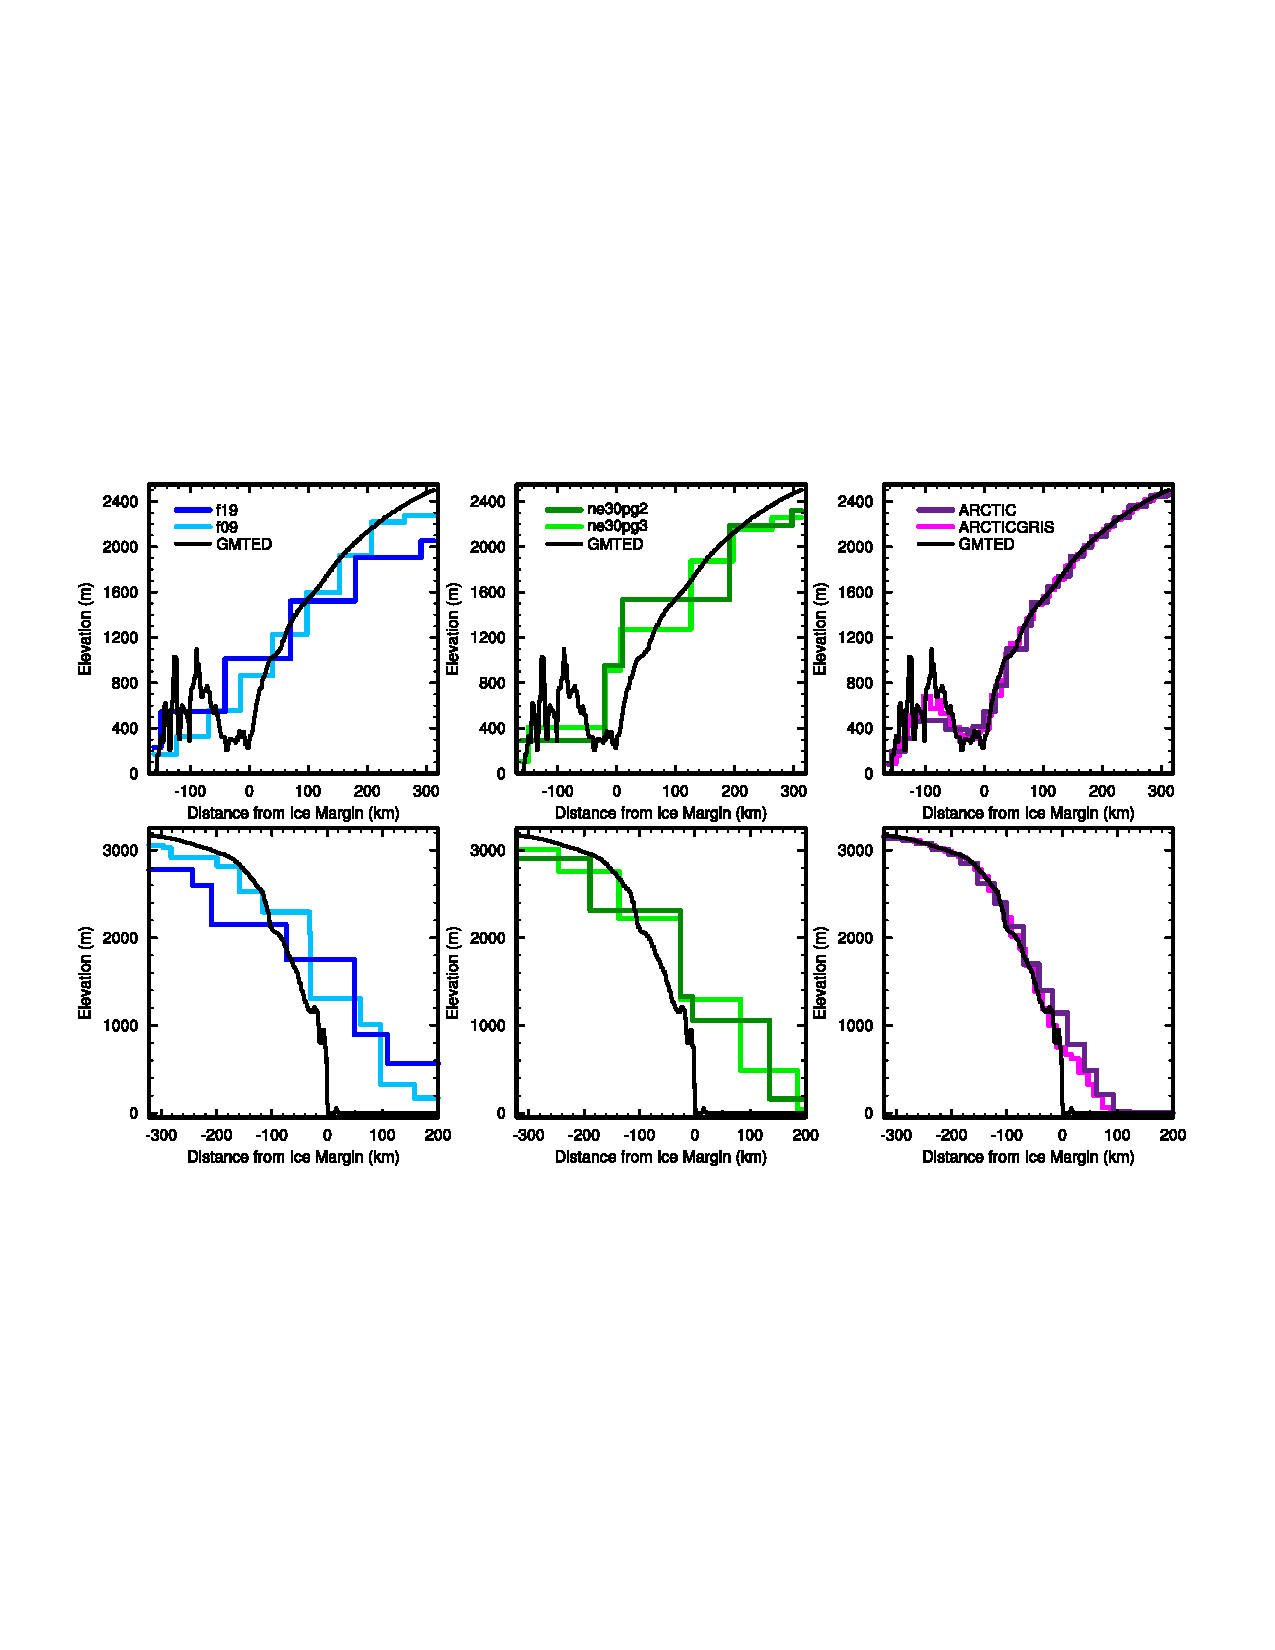
\includegraphics[width=130mm]{figs/temp_zsects.pdf}
\end{tabular}
\end{center}
\caption{Model surface elevation along the (top) K-transect, and (bottom) a transect spanning the central dome down to the Kangerlussuaq glacier in southeast Greenland, for all model grids. The reference surface (GMTED) is a 1 km surface elevation dataset used for generating the CAM topographic boundary conditions. }
\label{fig:ztrans}
\end{figure}

The transects in Figure~\ref{fig:ztrans} show that the ice sheet surface on the coarse grids is not systematically lower than the true surface in ablation zones. Rather, the smoothing of the raw topography, necessary to prevent the model from instigating grid-scale modes, flattens the ice sheet, causing the lower-elevation ablation zones to extend beyond the true ice sheet margin, where they lie above the actual ice surface. The $\tt f19$ grid has the smoothest topography since its dynamics are coarsest (whereas $\tt f09$, $\tt ne30pg2$ and $\tt ne30pg3$ use identical smoothing), and has the flattest ice sheet. This suggests that if anything, coarser models will tend to elevate the ablation zones and depress melt rates.

Figure~\ref{fig:ztrans} also shows the ice margin boundary, illustrating that the ablation zone lies in a narrow horizontal band where the ice sheet rapidly plunges to sea-level. Due to this abrupt transition, coarse grids will commonly represent the ablation zone with grid cells containing mixtures of ice-covered and ice-free regions. We hypothesize that coarser models have larger melt biases
%despite the $ARCTCIGRIS$ having the warmest troposphere,
because summer melting is confined to these mixed ice/land/ocean grid cells. CLM deals with land heterogeneity in a complex and sophisticated manner, but CAM only sees a homogenized state due to volume averaging over the sub-grid mixture. Thus, warm ice-free land patches in a grid cell may unduly influence the climate over the entire grid cell, causing a warm bias over the ice-covered patch. ({\color{blue}{This is an interesting conclusion pointing to the need for better treatment of surface inhomogeneity in CAM.  This might be a way to compensate for coarse resolution in future CESM versions?}})

Figure~\ref{fig:bias} shows mean melt bias, relative to both RACMO datasets, conditionally sampled based on grid cell ice fraction in the GrIS region. Errors are computed using the common-ice-mask approach, meaning that all fields are mapped to the common masks, which define the grid cell ice fraction. The figure shows ({\color{blue}{Any idea why the errors are smaller in the cells with intermediate ice fraction?  I wouldn't have expected this.}}) that coarser grids generally have two peaks in ice fraction space; a bump in positive melting errors in the 0-20$\%$ range, and another in the fully ice-covered cells. Also shown are the $\pm 1$~standard deviation of the biases for each bin. They indicate that the biases in 0-20$\%$ bins are mostly contained in the positive bias region (a fractional bias greater than 0), whereas the fully-covered ice cells have a wider distribution, with many grid cells also containing negative melting biases. The excessive melting in the 0-20$\%$ ice fraction bins supports our hypothesis that the prevalence of mixed-grid cells in the ablation zone on coarse grids is responsible for their large melt bias.

{\color{green}{Rene - is the melt map consistent with the bin figure? Smallest errors are interior points which correspond to glacier fraction bin of 1, which the largest errors.}}
{\color{blue}{ARH - I can check. The bin figure is fractional change so its a different metric, which could explain the apparent inconsistency.}}

\begin{figure}[t]
\begin{center}
\begin{tabular}{cccc}
         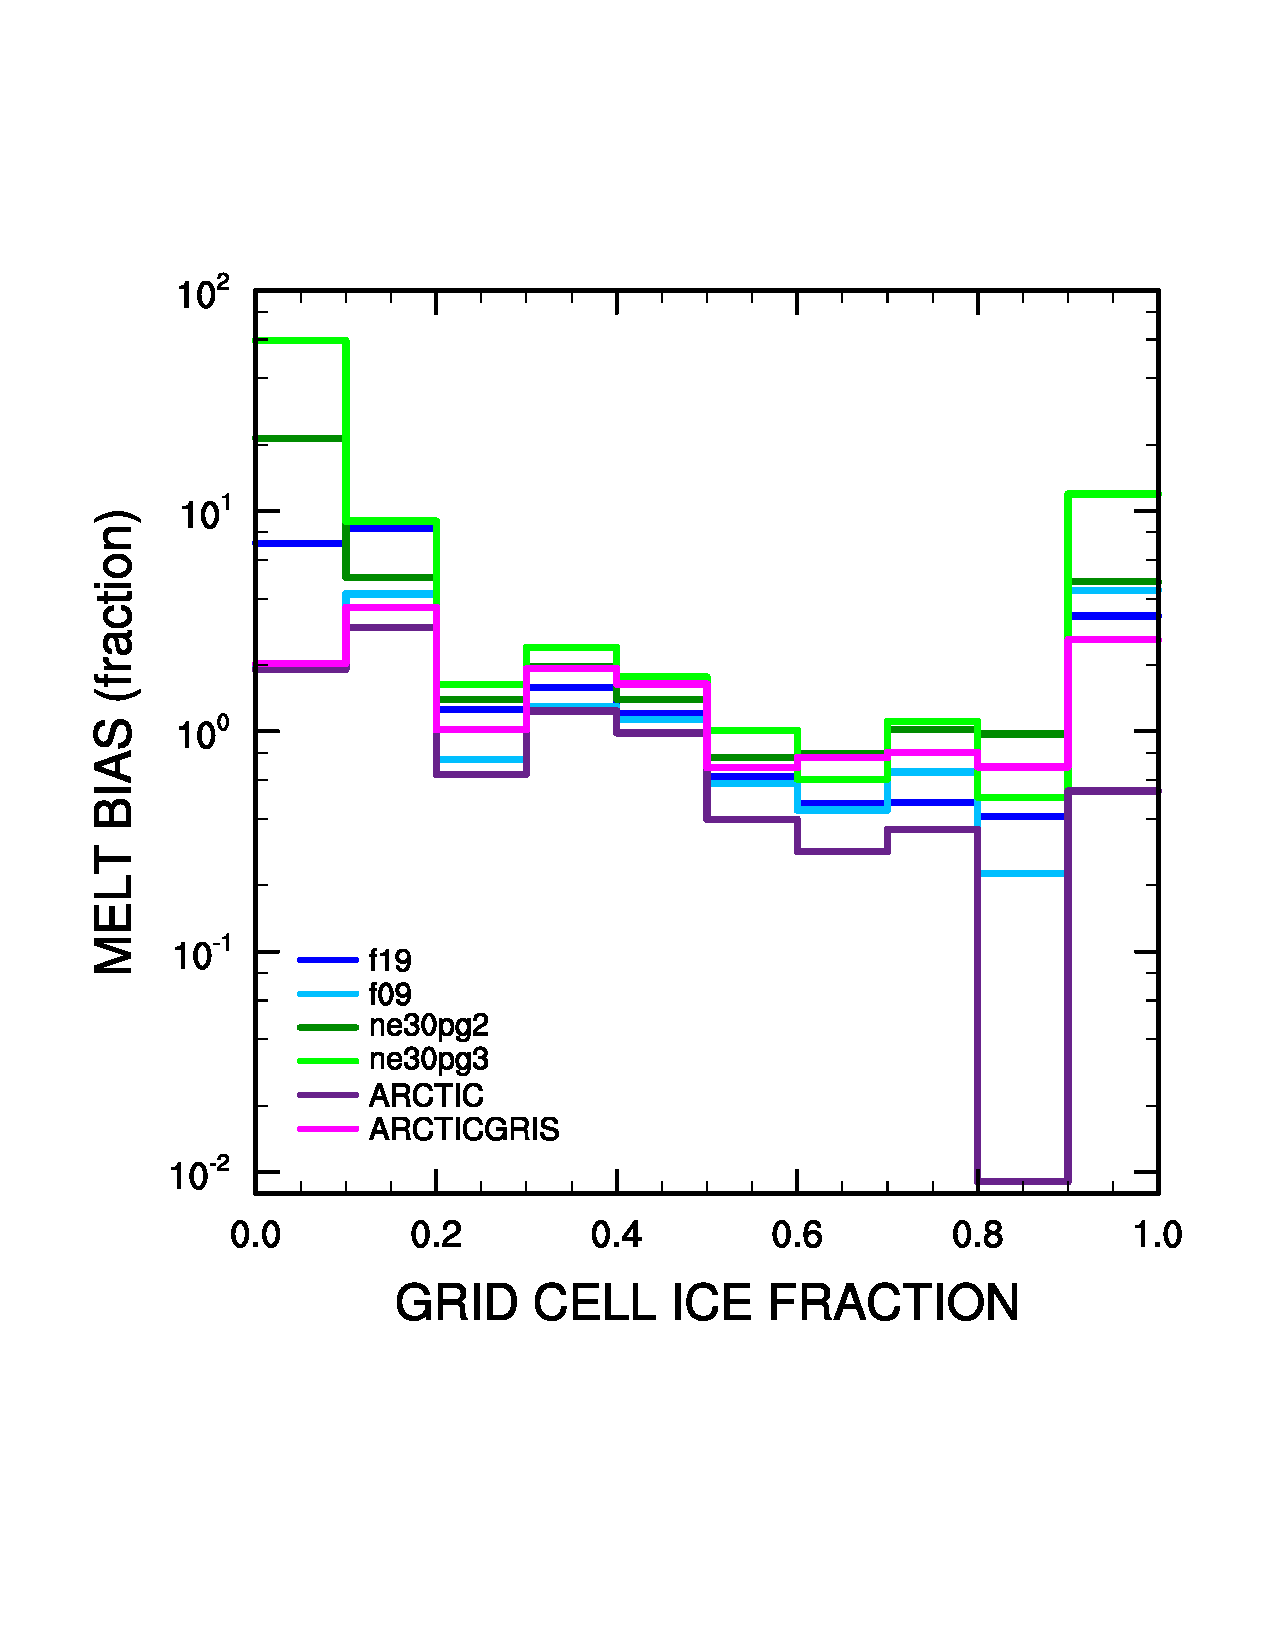
\includegraphics[width=80mm]{figs/temp_xy_diffRACMO_melt.pdf}
\end{tabular}
\end{center}
\caption{Fractional melt bias over the GrIS, computed relative to the RACMO datasets using the common ice mask approach, and conditionally sampled by grid cell ice fraction provided by the common ice masks. Solid lines are the mean of the distribution with $\pm$ one standard deviation expressed by shading.}
\label{fig:bias}
\end{figure}

\subsection{Precipitation extremes}

Synoptic storms are tracked using TempestExtremes atmospheric feature detection software \cite{UETAL2021}. As the $\tt Arctic$ grid contains $1/4^{\circ}$ refinement north of about $45^{\circ}$ latitude, the storm tracker is applied to this region for the $\tt Arctic$ and $\tt ne30pg3$ runs to identify differences in storm characteristics due to horizontal resolution. The composite mean precipitation maps are similar between the two grids, and exhibit the iconic comma structure of synoptic cyclones (not shown).

Figure~\ref{fig:comp-pdf} shows monthly PDFs of the precipitation rates associated with storms. The PDFs are constructed by sampling all the precipitation rates within $30^{\circ}$ of the storm center, for each point on the storm track and for all storms. The PDFs are evaluated on an identical composite grid for all runs, and so storm statistics are not impacted by differences in output resolution. The $\tt Arctic$ run has larger extreme precipitation rates compared to $\tt ne30pg3$ in every month, but the increase is greatest in the summer months, which coincides with the most extreme events of the year. This is primarily due to increased resolution and not the reduced physics times-step; the $\tt ne30pg3^{*}$ run only marginally increases the extreme precipitation rates compared with $\tt ne30pg3$ (Figure~\ref{fig:comp-pdf}).

The extreme precipitation rates in the $\tt Arctic$ run are closer than $\tt ne30pg3$ to the ERA5 reanalysis (Figure~\ref{fig:comp-pdf}). It is difficult to know how much the extreme precipitation rates in ERA5 are constrained by data assimilation, or whether these precipitation rates are due to using a similar $1/4^{\circ}$ model as the $\tt Arctic$ grid. However, it is well documented that $1/4^{\circ}$ models are more skillful at simulating extreme events \cite{BetAl2013JC,OETAL2016JAMES}.  This is an additional benefit of the VR grids.

\begin{figure}[t]
\begin{center}
         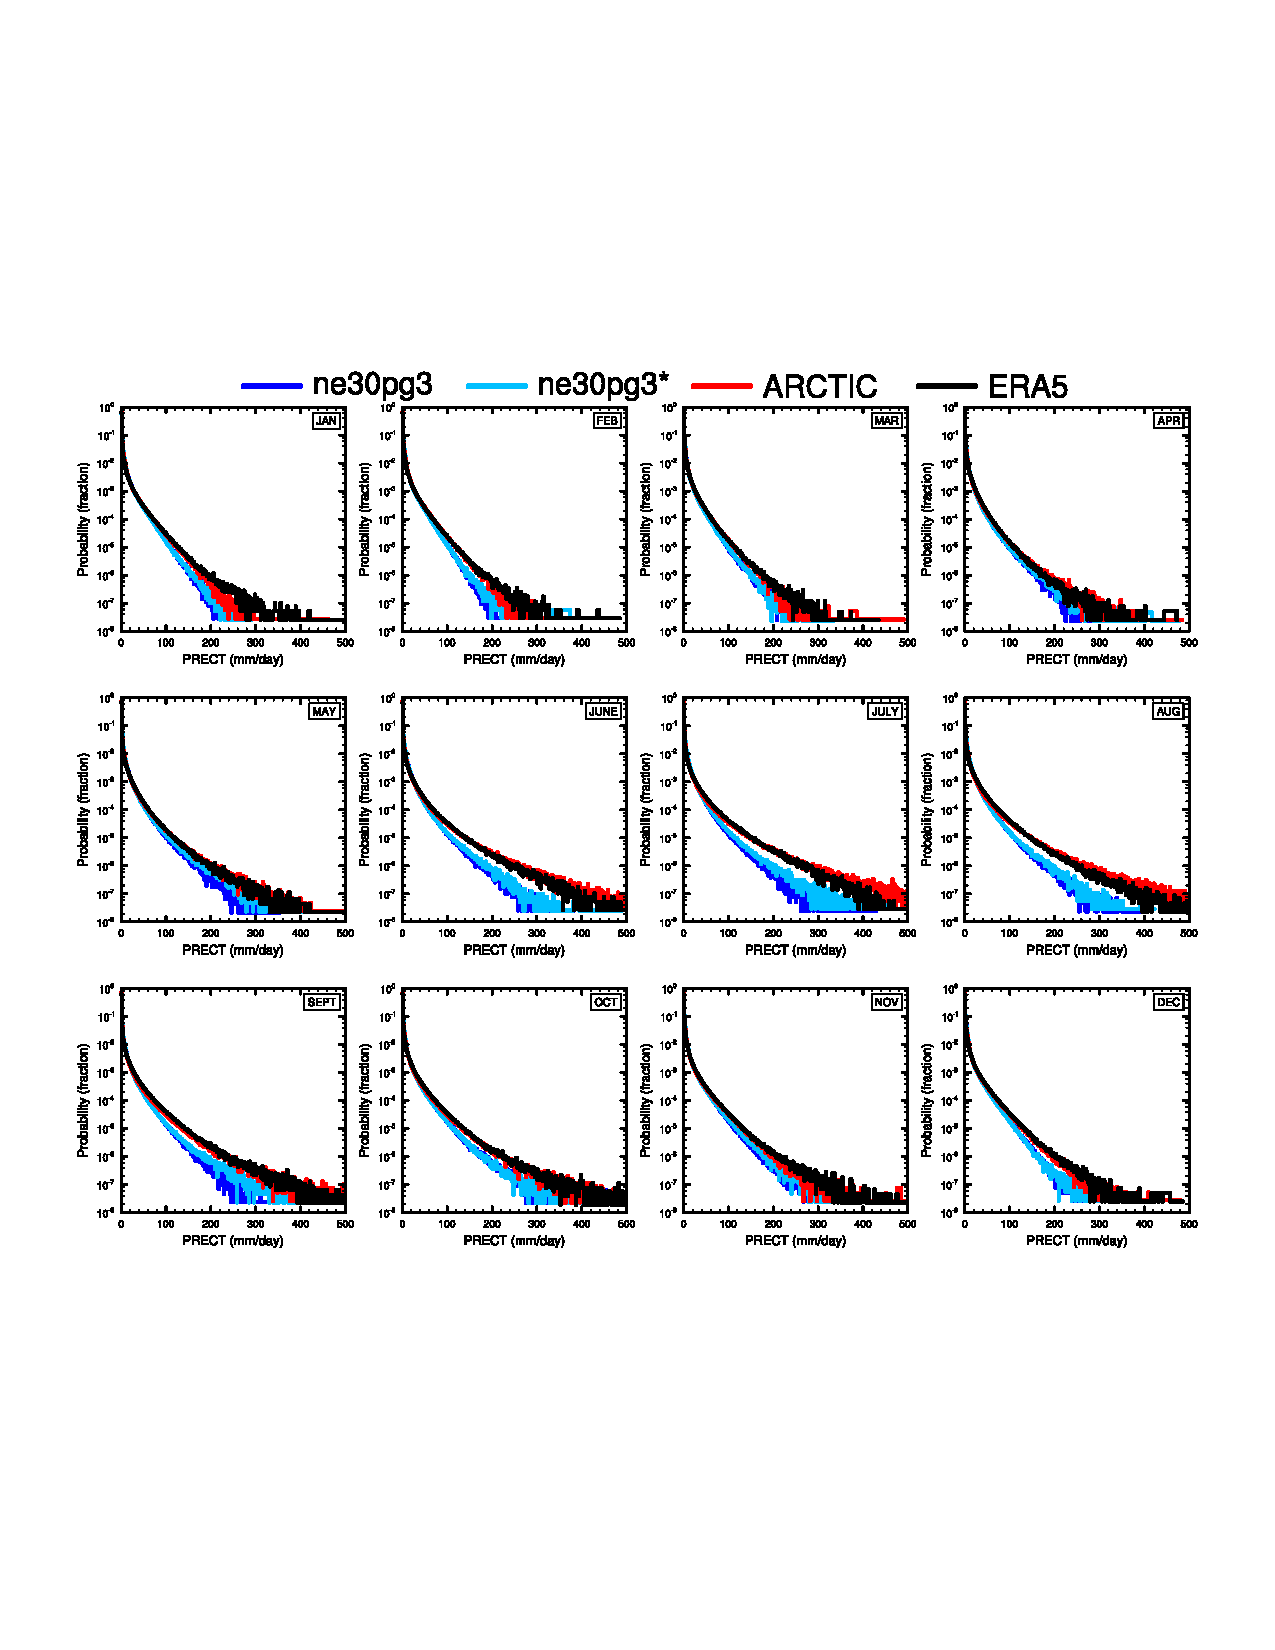
\includegraphics[width=130mm]{figs/temp_composite_ge45N_pdf.pdf}
\end{center}
\caption{PDFs of the total precipitation rate associated with tracked storms, by month, in the $\tt ne30pg3$, $\tt ne30pg3^{*}$ and $\tt Arctic$ runs, and compared with the ERA5 dataset.}
\label{fig:comp-pdf}
\end{figure}

\section{Conclusions}\label{sec:conclusions}

Running CESM2.2 in an AMIP-style configuration, we have evaluated six grids from two dynamical cores for their performance over the Arctic and in simulating the Greenland Ice Sheet (GrIS) surface mass balance (SMB). The $1-2^{\circ}$ finite-volume grids have enhanced resolution over polar regions due to the convergence of meridian lines, although a polar filter is used to prevent spurious atmospheric features from forming at this higher resolution. Spectral-element grids comparable to the resolution of the finite-volume grids have an isotropic grid structure, meaning the grid resolution is similar over the entire domain.
We developed two VR grids and introduced them into CESM2.2 as part of this work. Both use the spectral-element dycore; the $\tt Arctic$ grid has $1/4^{\circ}$ refinement over the broader Arctic, whereas the $\tt Arctic-GrIS$ grid is identical except for a $1/8^{\circ}$ patch of refinement over Greenland.

In general, the FV grids have colder summer temperatures over the Arctic compared with the SE grids (including the VR grids). The cloud biases in all the uniform-resolution grids, whether FV or SE, are similar, in general being too cloudy over Arctic land masses. The VR grids reduce the cloud biases. It should be emphasized that our analysis is specific to the Arctic summer because of its relevance to GrIS melt rates; improved clouds in the Arctic do not imply improved clouds at lower latitudes.

At the regional level, there is a halo of negative cloud bias (/color{blue}{I got confused about signs here, because section 3 talks about a halo of positive cloud SW forcing bias, which corresponds to a negative bias in cloud amounts.  Maybe replace 'cloud bias' with 'cloudiness bias' or something similar?}) around the ocean perimeter of Greenland on all $1-2^{\circ}$ grids, but not the VR grids. This halo bias coincides with a positive cloud bias over the ice sheet interior. This pattern has been traced to the inadequacy of the coarser grids for resolving orographic precipitation.  With overly smooth topography on the $1-2^{\circ}$ grids, synoptic systems moving into Greenland are not sufficiently lifted when encountering the steep ice margins.
As a result, moisture penetrates and dumps excess precipitation into the GrIS interior, instead of being concentrated near the coastal margins as shown by observations. This results in a positive precipitation and cloud bias in the ice sheet interior, and a halo of low cloud bias about the perimeter. The agreement of different observational data products on this bias lends confidence in the attribution of causes.
The VR grids compare better to the observations and show that orographic precipitation in Greenland is largely resolved.

We integrated the primary source and sink terms of the SMB equation over the GrIS for each of the six grids. The uniform $1-2^{\circ}$ grids have large positive accumulation biases because they fail to resolve orographic precipitation. The uniform SE grids have larger accumulation biases, suggesting that the FV grids are more skillful for precipitation due to finer resolution over Greenland, despite a polar filter. The VR grids have the most accurate accumulation rates of all the grids. 

The primary mass sink term of the GrIS, ice/snow melt, has similar biases. The uniform resolution SE grids have too much melt, while the FV grids have smaller biases. It is difficult to attribute these biases to grid resolution alone.  The FV grids have colder summers, consistent with their lower melt bias. However, the $\tt Arctic-GrIS$ grid has the warmest summer temperatures of all grids, yet it has less melting than the uniform-resolution SE grids. This suggests that grid resolution is responsible for a large fraction of the melt biases. We propose a mechanism: Coarse grids represent ablation zones using grid cells with mixed surface types, ice-covered and ice-free.  The warmer ice-free patches may largely determine the mean state, leading to a warm bias over the ice-covered patches of the grid cell. This mechanism is supported by analysis of melt biases binned by grid-cell ice fraction. 

The $\tt Arctic$ grid substantially improves the simulated Arctic climate, including precipitation extremes and the Greenland SMB, compared to the uniform $1^{\circ}-2^{\circ}$ grids. The $\tt Arctic-GrIS$ grid has the most realistic cloud and precipitation fields, but its summer temperatures are too warm. The $1^{\circ}$ FV model gives a surprisingly realistic SMB, likely due to the relatively fine resolution of Greenland on lat-lon grids. In particular, a greater number of grid cells in the ablation zone reduces the influence of mixed ice-covered/ice-free grid cells that represent ablation poorly on the other uniform-resolution grids.

As modeling systems move away from lat-lon grids towards quasi-uniform unstructured grids, it is worth taking stock of whether this will degrade the simulated polar climate. We have found that the $1^{\circ}$ FV model has clear advantages over the $1^{\circ}$ SE model in simulating the surface mass balance of the GrIS. This finding will not interrupt the ongoing transition towards unstructured grids in CESM, largely driven by gains in computational efficiency, but it has inspired us to develop alternative configurations that recover or improve on the fidelity of polar climate. We have shown here (and in a prior companion study \cite{VETAL2018TC}) that for CESM, Arctic-refined meshes can substantially improve the simulated mass balances of the GrIS, even compared to the $1^{\circ}$ grid. This should reassure the CESM modeling community that the ongoing transition away from lat-lon grids will not adversely impact CESM's usefuless as a state-of-the-art tool for simulating and understanding polar processes.
{\color{blue} (WHL: This last sentence may be too sanguine.  Yes, we can recover the fidelity of Arctic simulations using VR grids, but (so far) only at a considerable cost in cpu-hours.  This points to the need for an intermediate resolution that is more affordable, and/or model development or tuning that reduces the biases on coarse grids.)}{\color{purple}{Andrew - Maybe better to just state that higher resolution is better: 1deg better than 2deg FV, and ne30 is coarser than 1deg at Greenland latitudes so it's worse. But VR has higher resolution so SR-VR is better. It's all about resolution.}}

We are  working to develop a configuration of the $\tt Arctic$ grid that is fully-coupled with the CESM ocean and sea ice components and the Community Ice Sheet Model (CISM), to provide multi-century projections of the state of the GrIS and its contribution to sea-level rise.
%A fully-coupled pre-industrial control configuration has already been developed and vetted.
%, and should be incorporated into CESM in the near future.
We have also developed a visualization of the $ARCTCGRIS$ run, now available on youtube\footnote{\url{https://www.youtube.com/watch?v=YwHgqDu75s8&t=4s&ab_channel=NCARVisLab}}.
%in order to advertise some of the stunning capabilities of the refined mesh approach.
Figure~\ref{fig:viz} shows a snapshot of this visualization, illustrating mesoscale katabatic winds descending the southeastern slopes of GrIS.
%We are optimistic about the polar science opportunities provided by these new Arctic mesh configurations, and our open to collaborating with the CESM community to assist in anyway we can.
These new grids and configurations will provide new opportunities for CESM polar science and aims to contribute to an improved understanding of the polar environment.
{\color{blue} (WHL: I replaced the previous last sentence because it seemed too much like an advertisement.  However, this new ending seems weak.  I wonder if we should say something about future work motivated by this study, for instance investigating grids and parameterizations that provide some of the same benefits as these VR grids but at lower cost.)}

\begin{figure}[t]
\begin{center}
         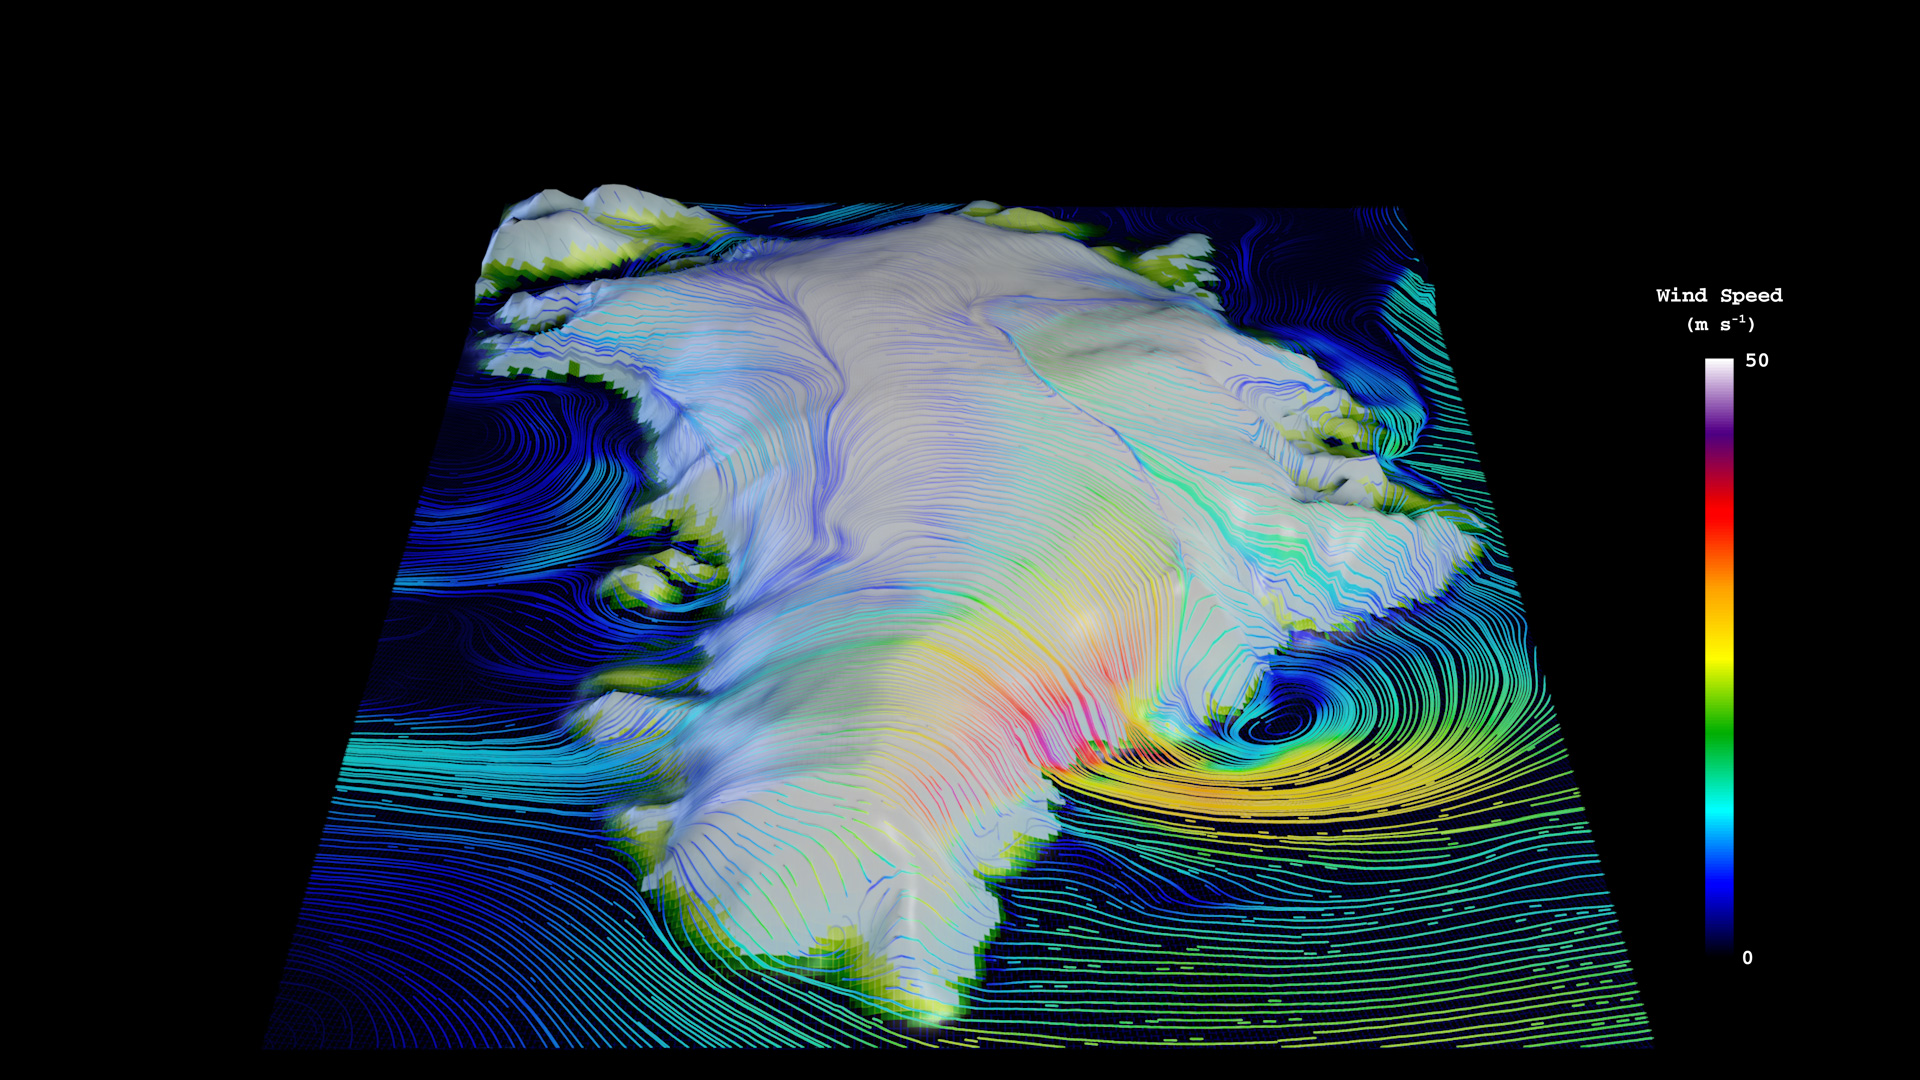
\includegraphics[width=130mm]{figs/Vis1472.jpg}
\end{center}
\caption{Snapshot of the lowest model level streamlines from the $\tt Arctic-GrIS$ visualization, with color shading denoting the wind magnitude.}
\label{fig:viz}
\end{figure}

% \section{Materials and Methods}
% Here is text on Materials and Methods.
%
% \subsection{A descriptive heading about methods}
% More about Methods.
%
% \section{Data} (Or section title might be a descriptive heading about data)
%
% \section{Results} (Or section title might be a descriptive heading about the
% results)
%

%\begin{figure}[t]
%\begin{center}
%         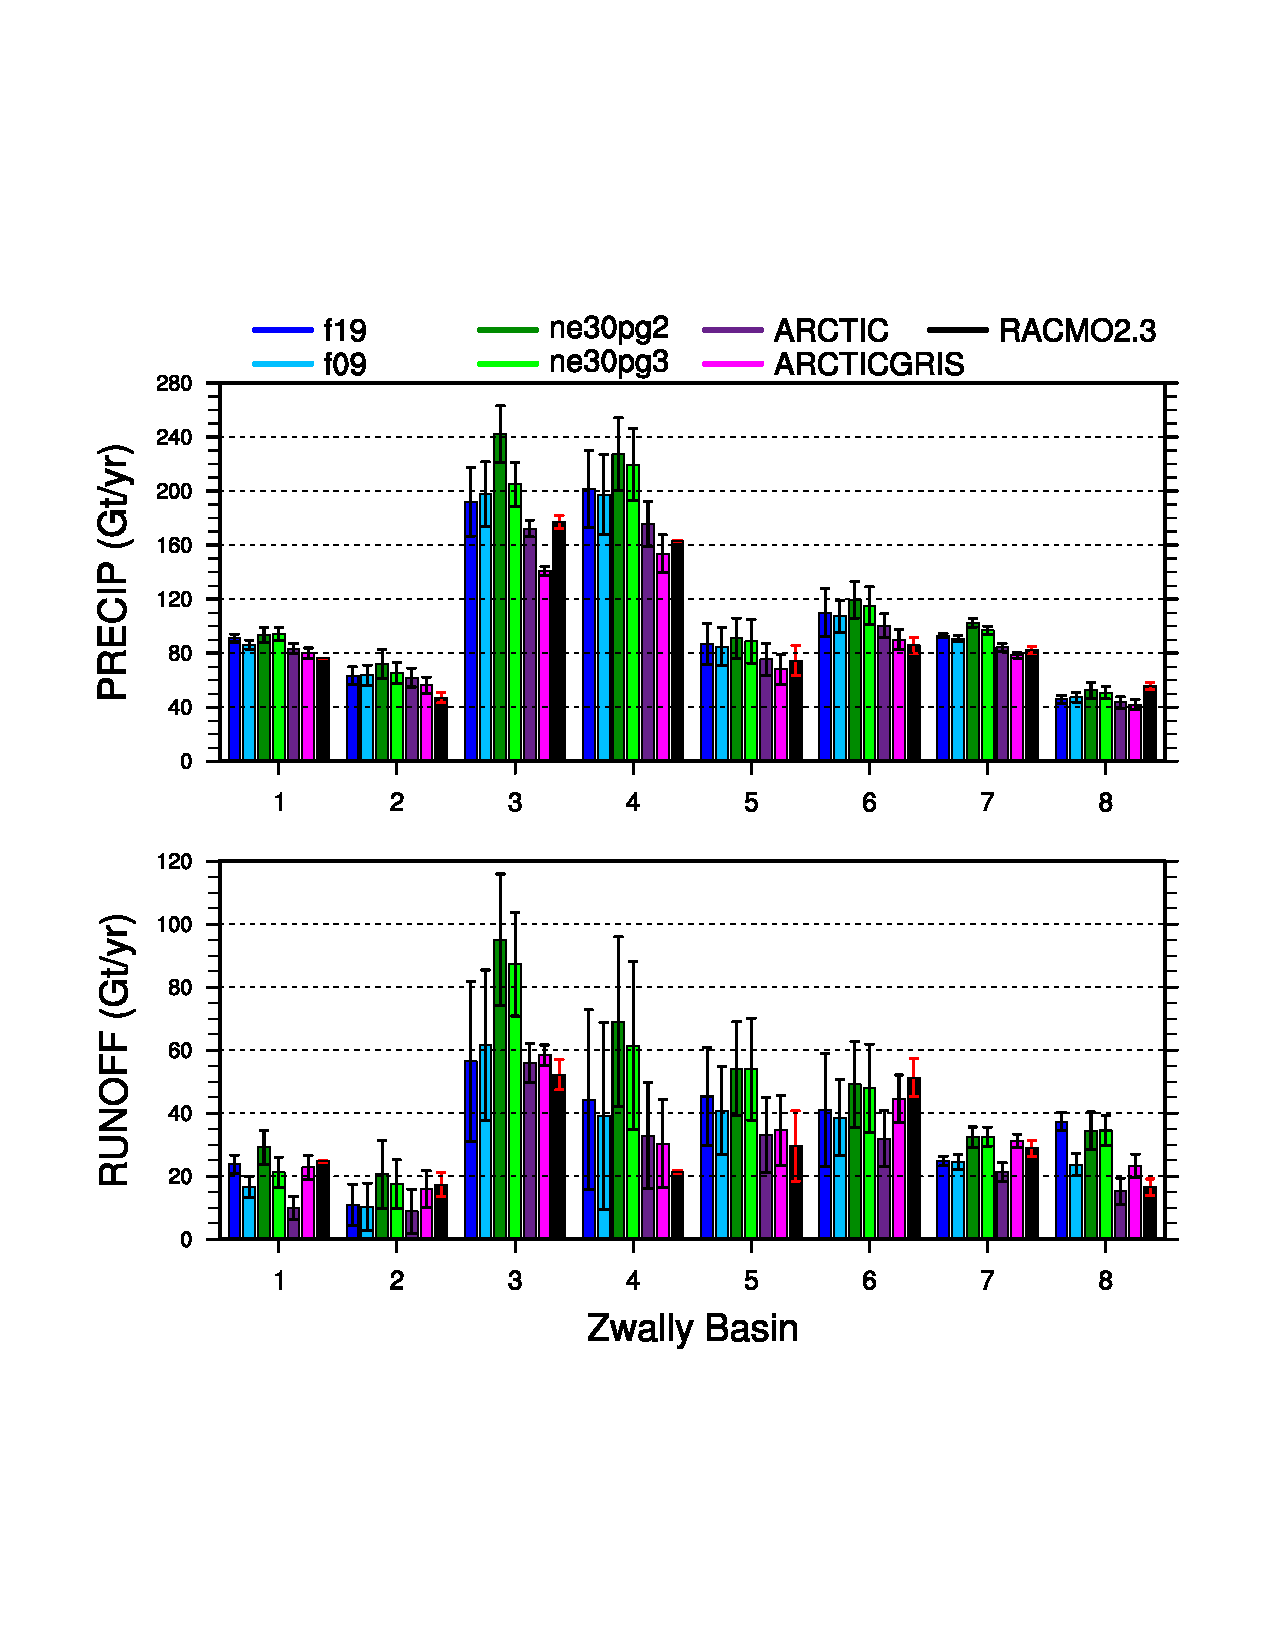
\includegraphics[width=100mm]{figs/temp_tseries_BASIN_uqmap.pdf}
%\end{center}
%\caption{.}
%\label{fig:zwally}
%\end{figure}

%Text here ===>>>


%%

%  Numbered lines in equations:
%  To add line numbers to lines in equations,
%  \begin{linenomath*}
%  \begin{equation}
%  \end{equation}
%  \end{linenomath*}



%% Enter Figures and Tables near as possible to where they are first mentioned:
%
% DO NOT USE \psfrag or \subfigure commands.
%
% Figure captions go below the figure.
% Table titles go above tables;  other caption information
%  should be placed in last line of the table, using
% \multicolumn2l{$^a$ This is a table note.}
%
%----------------
% EXAMPLE FIGURES
%
% \begin{figure}
% \includegraphics{example.png}
% \caption{caption}
% \end{figure}
%
% Giving latex a width will help it to scale the figure properly. A simple trick is to use \textwidth. Try this if large figures run off the side of the page.
% \begin{figure}
% \noindent\includegraphics[width=\textwidth]{anothersample.png}
%\caption{caption}
%\label{pngfiguresample}
%\end{figure}
%
%
% If you get an error about an unknown bounding box, try specifying the width and height of the figure with the natwidth and natheight options. This is common when trying to add a PDF figure without pdflatex.
% \begin{figure}
% \noindent\includegraphics[natwidth=800px,natheight=600px]{samplefigure.pdf}
%\caption{caption}
%\label{pdffiguresample}
%\end{figure}
%
%
% PDFLatex does not seem to be able to process EPS figures. You may want to try the epstopdf package.
%

%
% ---------------
% EXAMPLE TABLE
%
% \begin{table}
% \caption{Time of the Transition Between Phase 1 and Phase 2$^{a}$}
% \centering
% \begin{tabular}{l c}
% \hline
%  Run  & Time (min)  \\
% \hline
%   $l1$  & 260   \\
%   $l2$  & 300   \\
%   $l3$  & 340   \\
%   $h1$  & 270   \\
%   $h2$  & 250   \\
%   $h3$  & 380   \\
%   $r1$  & 370   \\
%   $r2$  & 390   \\
% \hline
% \multicolumn{2}{l}{$^{a}$Footnote text here.}
% \end{tabular}
% \end{table}

%% SIDEWAYS FIGURE and TABLE
% AGU prefers the use of {sidewaystable} over {landscapetable} as it causes fewer problems.
%
% \begin{sidewaysfigure}
% \includegraphics[width=20pc]{figsamp}
% \caption{caption here}
% \label{newfig}
% \end{sidewaysfigure}
%
%  \begin{sidewaystable}
%  \caption{Caption here}
% \label{tab:signif_gap_clos}
%  \begin{tabular}{ccc}
% one&two&three\\
% four&five&six
%  \end{tabular}
%  \end{sidewaystable}

%% If using numbered lines, please surround equations with \begin{linenomath*}...\end{linenomath*}
%\begin{linenomath*}
%\begin{equation}
%y|{f} \sim g(m, \sigma),
%\end{equation}
%\end{linenomath*}

%%% End of body of article

%%%%%%%%%%%%%%%%%%%%%%%%%%%%%%%%
%% Optional Appendix goes here
%
% The \appendix command resets counters and redefines section heads
%
% After typing \appendix
%
%\section{Here Is Appendix Title}
% will show
% A: Here Is Appendix Title
%
\appendix
\section{Details on spectra-element dynamical core improvements since the CESM2.0 release}
Since the CESM2.0 release of the spectral-element dynamical core documented in \citeA{LetAl2018JAMES} some important algorithmic improvements have been implemented and released with CESM2.2. These pertain mainly to the flow over orography that, for the spectral-element dynamical core, can lead to noise aligned with the element boundaries \cite{HL2018MWR}.
\subsection{Reference profiles}
Significant improvement in removing noise for flow over orography can be achieved by using reference profiles for temperature and pressure
\begin{eqnarray}
  T^{(ref)}&=&T_0+T_1 \Pi^{(ref)},\\
  p_s^{(ref)}&=&p_0\exp{\left(-\frac{\Phi_s}{R^{(d)}(T_0+T_1)}\right)},
\end{eqnarray}
{\color{blue}{Mark - Note: new definition of T0 means this equation should also be changed}} \cite{SJ1991QJRMS} where $g$ gravity, $T_1=\Gamma_0 T_0 c_p^{(d)}/g\approx 192K$ with standard lapse rate $\Gamma_0\equiv 6.5K/km$ and $T_0\equiv 288K-T_0\approx 97K$ ($c_p^{(d)}$ specific heat of dry air at constant pressure; $R^{(d)}$ gas constant for dry air), and $\Phi_s$ surface geopotential. The reference Exner function is
\begin{equation}
   \Pi^{(ref)}=\left( \frac{p^{(ref)}}{p_0}\right)^{\kappa}
\end{equation}
where $\kappa=\frac{R^{(d)}}{c_p^{(d)}}$. The reference surface pressure $p_0=1000hPa$ and at each model level the reference pressure $p^{(ref)}$ is computed from $p_s^{(ref)}$ and the standard hybrid coefficients
\begin{equation}
    p^{(ref)}(\eta) = A(\eta)p_0+B(\eta)p_s^{(ref)},
\end{equation}
where $A$ and $B$ are the standard hydrid coefficients (using a dry-mass generalized vertical mass coordinate $\eta$). These reference profiles are subtracted from the prognostic temperature and pressure-level-thickness states before applying hyperviscosity:
\begin{eqnarray}
   \hbox{CESM2.0}&\rightarrow&\hbox{CESM2.2}\\
   && \\
  \nabla^4_\eta T &\rightarrow& \nabla^4_\eta \left(T-T^{(ref)}\right),\label{eq:hyperT}\\ 
    \nabla^4_\eta \delta p^{(d)} &\rightarrow& \nabla^4_\eta \left(\delta p^{(d)}-\delta p^{(ref)}\right).\label{eq:hyperDP}
\end{eqnarray}
This reduces spurious transport of temperature and mass up/down-slope due to the hyperviscosity operator. 


\subsection{Rewriting the pressure gradient force (PGF)}
In the CESM2.0 the following (standard) form of the pressure gradient term was used:
\begin{equation}
\label{eq:pgf}
    \nabla_{\eta }\Phi+\frac{1}{\rho}\nabla_{\eta }p,
\end{equation}
where $\Phi$ is geopotential and $\rho=\frac{R^{(d)}T_v}{p}$ is density \cite<for details see >{LetAl2018JAMES}. To alleviate noise for flow over orography, 
 we switched to an Exner pressure formulation following \citeA{T2020JAMES}, which uses that (\ref{eq:pgf}) can be written in terms of the Exner pressure
\begin{equation}\label{eq:pgf2}
    \nabla_{\eta }\Phi+c_p^{(d)}\theta_v\nabla_{\eta }\Pi,
\end{equation}
where the Exner pressure is
\begin{equation}
    \Pi\equiv \left( \frac{p}{p_0}\right)^{\kappa}.
\end{equation}
The derivation showing that (\ref{eq:pgf}) and (\ref{eq:pgf2}) are equivalent is shown here:
\begin{eqnarray*}
c_p^{(d)}\theta_v\nabla_{\eta }\Pi &=& c_p^{(d)}\theta_v\nabla_{\eta }\left( \frac{p}{p_0}\right)^{\kappa},\\
&=& c_p^{(d)}\theta_v\kappa\left( \frac{p}{p_0}\right)^{\kappa-1} \nabla_{\eta }\left( \frac{p}{p_0}\right),\\
&=& c_p^{(d)}\theta_v\kappa\Pi\left( \frac{p_0}{p}\right) \nabla_{\eta }\left(\frac{p}{p_0}\right),\\
&=& \frac{c_p^{(d)}\theta_v\kappa\Pi}{p} \nabla_{\eta }p,\\
&=& \frac{R^{(d)}\theta_v\Pi}{p} \nabla_{\eta }p,\\
&=& \frac{R^{(d)}T_v}{p} \nabla_{\eta }p,\\
&=& \frac{1}{\rho} \nabla_{\eta }p.
\end{eqnarray*}
Using the reference states from \cite{SJ1991QJRMS},
\begin{eqnarray}
  \overline{T}&=&T_0+T_1 \Pi,\\
  \overline{\theta}&=&{T_0}/\Pi+T_1,
\end{eqnarray}
we can define a geopotential as a function of Exner pressure
\begin{equation}
    \overline{\Phi} = -c_p^{(d)}\left( T_0\log \Pi+T_1\Pi-T_1\right). 
\end{equation}
This "balanced" geopotential obeys
\begin{equation}
    c_p^{(d)}\overline{\theta}\nabla \Pi+\nabla \overline{\Phi}=0 
\end{equation}
for any Exner pressure. Subtracting this "reference" profile from the PGF yields
\begin{eqnarray}
    \nabla_{\eta }\Phi+c_p^{(d)}\theta_v\nabla_{\eta }\Pi&=& \nabla_{\eta }\left(\Phi-\overline{\Phi}\right)+c_p^{(d)}\left(\theta_v-\overline{\theta}\right)\nabla_{\eta }\Pi,\nonumber \\
    &=& \nabla_{\eta }\Phi+c_p^{(d)}\theta_v\nabla_{\eta }\Pi+c_p^{(d)}T_0\left[ \nabla_\eta \log \Pi -\frac{1}{\Pi}\nabla_\eta \Pi\right].\label{eq:pgf_ref}
\end{eqnarray}
In the continuum, the two formulations (left and right-hand side of (\ref{eq:pgf_ref})) are identical. But under discretization, the second formulation can have much less truncation error. 

\subsection{Results}
{\color{red}{[Adam: have you defined ne30np4 in the main text?]}}\\
One year averages of vertical pressure velocity at 500hPa ( {\tt OMEGA500}) have been found to be a useful quantity to detect spurious up or down-drafts induced by steep orography (Figure \ref{fig:OMEGA500}). While the true solution is not known, strong vertical velocities aligned with element edges that are not found in the CAM-FV reference solution (Figure \ref{fig:OMEGA500}(a)) are likely not physical (spurious). The older CESM2.0 version of SE (Figure \ref{fig:OMEGA500}(d)) using the "traditional" discretization of the PGF, (\ref{eq:pgf_ref}), exhibits significant spurious noise patters around steep orography compared to CAM-FV (e.g., around Himalayas and Andes). This is strongly alleviated by switching to the Exner formulation of the PGF (\ref{eq:pgf2}; Figure \ref{fig:OMEGA500}(c)). By also subtracting reference profiles from pressure-level thickness and temperature, equations (\ref{eq:hyperT}) and (\ref{eq:hyperDP}) respectively, reduces strong up-down drafts further (Figure \ref{fig:OMEGA500}(d)). Switching to the CAM-SE-CSLAM version where physics tendencies are computed on an quasi-equal area physics grid and using the CSLAM transport scheme, marginal improvements are observed in terms of a smoother vertical velocity field (Figure \ref{fig:OMEGA500}(e,f)). The configuration shown in Figure \ref{fig:OMEGA500}(d) is used for the simulations shown in the main text of this paper.

It is interesting to note that the noise issues and algorithmic remedies found in the real-world simulations discussed above, can be investigated by replacing all of physics with a modified version of the Held-Suarez forcing \cite{HS1994}. The original formulation of the Held-Suarez idealized test case used a flat Earth ($\Phi_s=0$) and a dry atmosphere. By simply adding the surface topography used in `real-world' simulations and removing the temperature relaxation in the lower part of domain ($\sigma>0.7$; see \citeA{HS1994} for details), surprisingly realistic vertical velocity fields (in terms of structure) result (see Figure \ref{fig:OMEGA500FHS94}). Since this was a very useful development tool it is shared in this manuscript. 

\begin{figure}[t]
\begin{center}
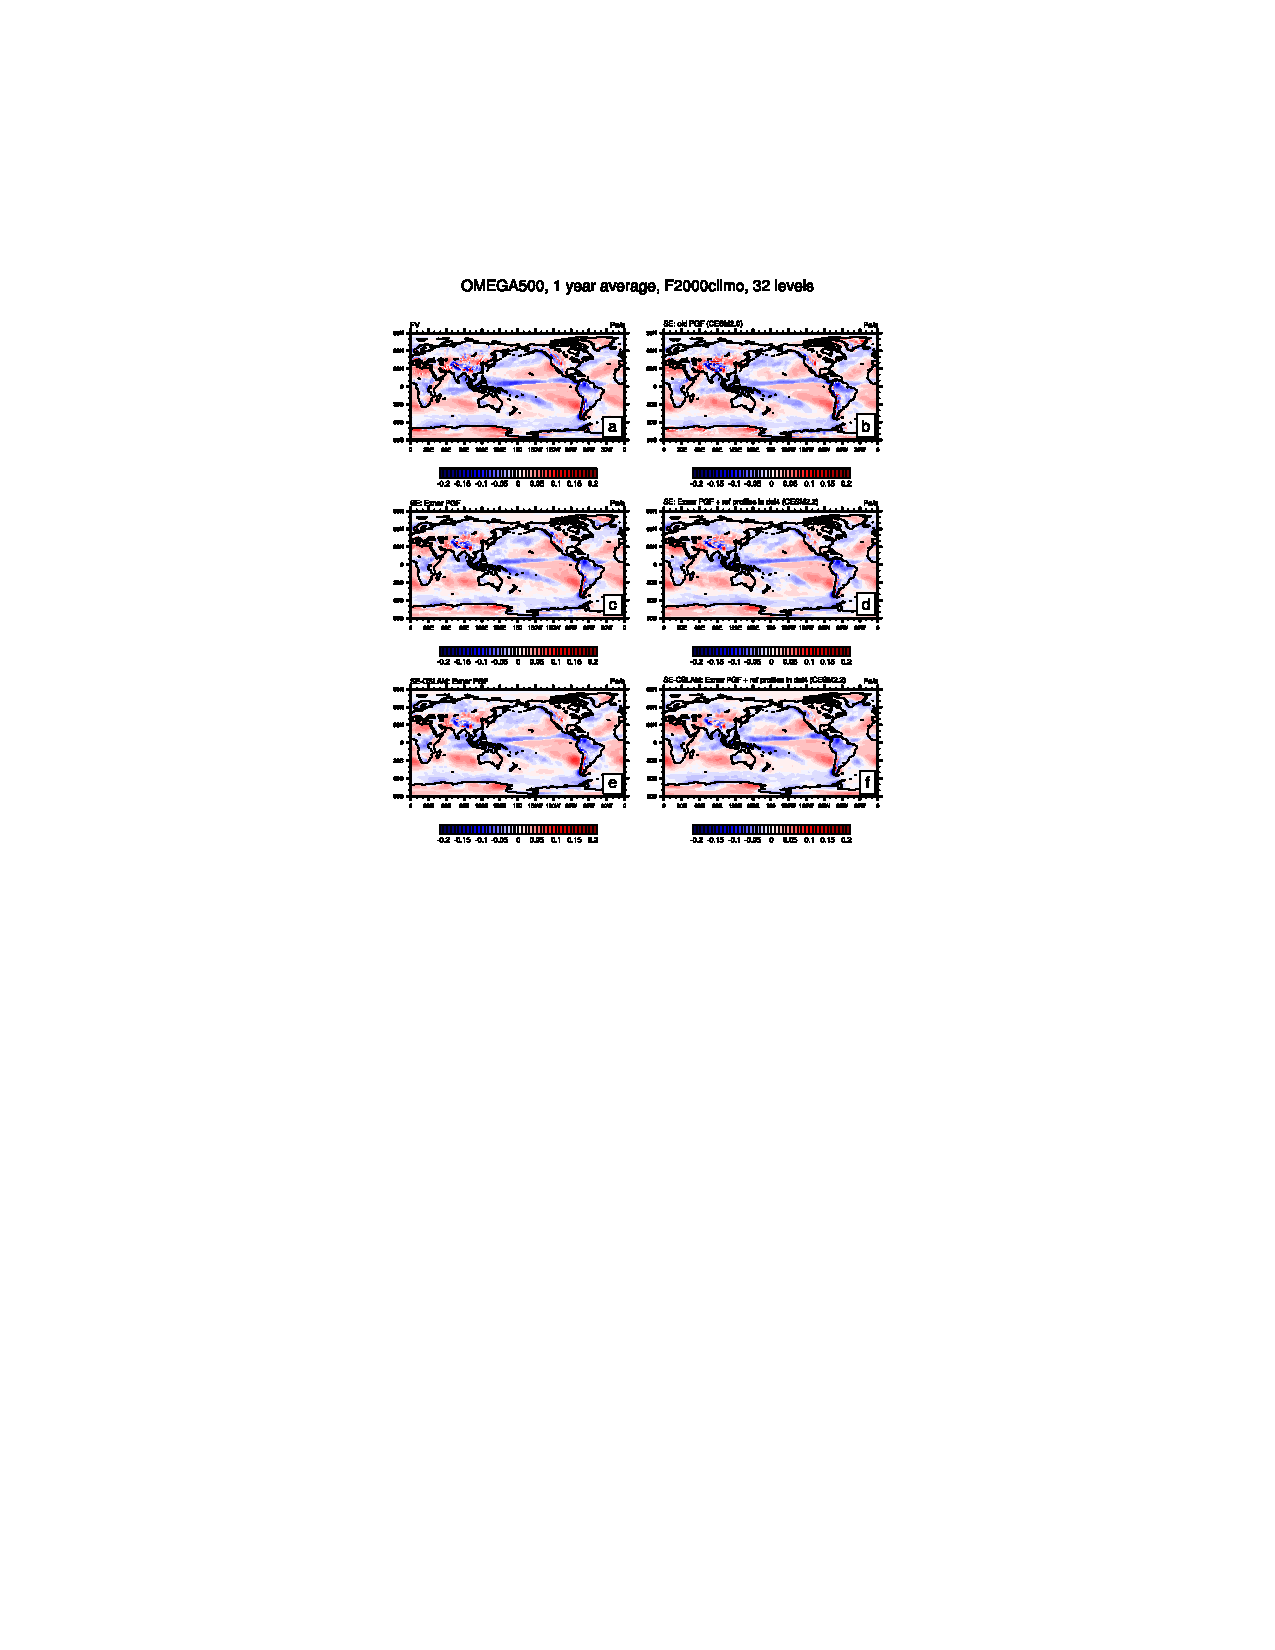
\includegraphics[width=145mm]{OMEGA500F2000climo.pdf}
\end{center}
\caption{One year averages of vertical pressure velocity at 500hPa ({\tt OMEGA500}) using (a) CAM-FV (Finite-Volume dynamical core) and (b-f) various versions of the spectral-element (SE) dynamical core at approximately $1^\degree$ horizontal resolution and using 32 levels. (b) is equivalent to the CESM2.0 version of the SE dynamical core using the "traditional"/"old" discretization of the pressure-gradient force (PGF). Plot (c) is equivalent to configuration (b) but using the Exner form of the PGF. Plot (d) is the same as configuration (c) but also subtracting reference profiles from pressure and temperature before applying hyperviscosity operators (which is equivalent to the CESM2.2 version of SE in terms of the dynamical core). Plots (e) and (f) are equivalent to (c) and (d), respectively, by using the SE-CSLAM ($\tt ne30pg3$) version of the SE dynamical core (i.e. separate quasi-uniform physics grid and CSLAM transport scheme).}\label{fig:OMEGA500}
\end{figure}
\begin{figure}[t]
\begin{center}
\includegraphics[width=145mm]{OMEGA500FHS94.pdf}
\end{center}
\caption{Same as Figure \ref{fig:OMEGA500} but using modified Held-Suarez forcing and the average is over 18 months (excl. spin-up).}\label{fig:OMEGA500FHS94}
\end{figure}

%%%%%%%%%%%%%%%%%%%%%%%%%%%%%%%%%%%%%%%%%%%%%%%%%%%%%%%%%%%%%%%%
%
% Optional Glossary, Notation or Acronym section goes here:
%
%%%%%%%%%%%%%%
% Glossary is only allowed in Reviews of Geophysics
%  \begin{glossary}
%  \term{Term}
%   Term Definition here
%  \term{Term}
%   Term Definition here
%  \term{Term}
%   Term Definition here
%  \end{glossary}

%
%%%%%%%%%%%%%%
% Acronyms
%   \begin{acronyms}
%   \acro{Acronym}
%   Definition here
%   \acro{EMOS}
%   Ensemble model output statistics
%   \acro{ECMWF}
%   Centre for Medium-Range Weather Forecasts
%   \end{acronyms}

%
%%%%%%%%%%%%%%
% Notation
%   \begin{notation}
%   \notation{$a+b$} Notation Definition here
%   \notation{$e=mc^2$}
%   Equation in German-born physicist Albert Einstein's theory of special
%  relativity that showed that the increased relativistic mass ($m$) of a
%  body comes from the energy of motion of the body—that is, its kinetic
%  energy ($E$)—divided by the speed of light squared ($c^2$).
%   \end{notation}




%%%%%%%%%%%%%%%%%%%%%%%%%%%%%%%%%%%%%%%%%%%%%%%%%%%%%%%%%%%%%%%%
%
%  ACKNOWLEDGMENTS
%
% The acknowledgments must list:
%
% >>>>	A statement that indicates to the reader where the data
% 	supporting the conclusions can be obtained (for example, in the
% 	references, tables, supporting information, and other databases).
%
% 	All funding sources related to this work from all authors
%
% 	Any real or perceived financial conflicts of interests for any
%	author
%
% 	Other affiliations for any author that may be perceived as
% 	having a conflict of interest with respect to the results of this
% 	paper.
%
%
% It is also the appropriate place to thank colleagues and other contributors.
% AGU does not normally allow dedications.


\acknowledgments
    This material is based upon work supported by the National Center for Atmospheric Research (NCAR), which is a major facility sponsored by the NSF under Cooperative Agreement 1852977. Computing and data storage resources, including the Cheyenne supercomputer (doi:10.5065/D6RX99HX), were provided by the Computational and Information Systems Laboratory (CISL) at NCAR. A. Herrington thanks Matt Rehme (NCAR/CISL) for his role in generating the $\tt Arctic-GrIS$ visualization available on youtube ({\url{https://www.youtube.com/watch?v=YwHgqDu75s8&t=4s&ab_channel=NCARVisLab}}).

The data presented in main part of this manuscript is available at {\url{https://github.com/adamrher/2020-arcticgrids}}. The source code and data for the Appendix is available at {\url{https://github.com/PeterHjortLauritzen/CAM/tree/topo-mods}}.

%% ------------------------------------------------------------------------ %%
%% References and Citations

%%%%%%%%%%%%%%%%%%%%%%%%%%%%%%%%%%%%%%%%%%%%%%%
%
% \bibliography{<name of your .bib file>} don't specify the file extension
%
% don't specify bibliographystyle
%%%%%%%%%%%%%%%%%%%%%%%%%%%%%%%%%%%%%%%%%%%%%%%

%\bibliography{ enter your bibtex bibliography filename here }
\bibliography{bib}


%Reference citation instructions and examples:
%
% Please use ONLY \cite and \citeA for reference citations.
% \cite for parenthetical references
% ...as shown in recent studies (Simpson et al., 2019)
% \citeA for in-text citations
% ...Simpson et al. (2019) have shown...
%
%
%...as shown by \citeA{jskilby}.
%...as shown by \citeA{lewin76}, \citeA{carson86}, \citeA{bartoldy02}, and \citeA{rinaldi03}.
%...has been shown \cite{jskilbye}.
%...has been shown \cite{lewin76,carson86,bartoldy02,rinaldi03}.
%... \cite <i.e.>[]{lewin76,carson86,bartoldy02,rinaldi03}.
%...has been shown by \cite <e.g.,>[and others]{lewin76}.
%
% apacite uses < > for prenotes and [ ] for postnotes
% DO NOT use other cite commands (e.g., \citet, \citep, \citeyear, \nocite, \citealp, etc.).
%



\end{document}



More Information and Advice:

%% ------------------------------------------------------------------------ %%
%
%  SECTION HEADS
%
%% ------------------------------------------------------------------------ %%

% Capitalize the first letter of each word (except for
% prepositions, conjunctions, and articles that are
% three or fewer letters).

% AGU follows standard outline style; therefore, there cannot be a section 1 without
% a section 2, or a section 2.3.1 without a section 2.3.2.
% Please make sure your section numbers are balanced.
% ---------------
% Level 1 head
%
% Use the \section{} command to identify level 1 heads;
% type the appropriate head wording between the curly
% brackets, as shown below.
%
%An example:
%\section{Level 1 Head: Introduction}
%
% ---------------
% Level 2 head
%
% Use the \subsection{} command to identify level 2 heads.
%An example:
%\subsection{Level 2 Head}
%
% ---------------
% Level 3 head
%
% Use the \subsubsection{} command to identify level 3 heads
%An example:
%\subsubsection{Level 3 Head}
%
%---------------
% Level 4 head
%
% Use the \subsubsubsection{} command to identify level 3 heads
% An example:
%\subsubsubsection{Level 4 Head} An example.
%
%% ------------------------------------------------------------------------ %%
%
%  IN-TEXT LISTS
%
%% ------------------------------------------------------------------------ %%
%
% Do not use bulleted lists; enumerated lists are okay.
% \begin{enumerate}
% \item
% \item
% \item
% \end{enumerate}
%
%% ------------------------------------------------------------------------ %%
%
%  EQUATIONS
%
%% ------------------------------------------------------------------------ %%

% Single-line equations are centered.
% Equation arrays will appear left-aligned.

Math coded inside display math mode \[ ...\]
 will not be numbered, e.g.,:
 \[ x^2=y^2 + z^2\]

 Math coded inside \begin{equation} and \end{equation} will
 be automatically numbered, e.g.,:
 \begin{equation}
 x^2=y^2 + z^2
 \end{equation}


% To create multiline equations, use the
% \begin{eqnarray} and \end{eqnarray} environment
% as demonstrated below.
\begin{eqnarray}
  x_{1} & = & (x - x_{0}) \cos \Theta \nonumber \\
        && + (y - y_{0}) \sin \Theta  \nonumber \\
  y_{1} & = & -(x - x_{0}) \sin \Theta \nonumber \\
        && + (y - y_{0}) \cos \Theta.
\end{eqnarray}

%If you don't want an equation number, use the star form:
%\begin{eqnarray*}...\end{eqnarray*}

% Break each line at a sign of operation
% (+, -, etc.) if possible, with the sign of operation
% on the new line.

% Indent second and subsequent lines to align with
% the first character following the equal sign on the
% first line.

% Use an \hspace{} command to insert horizontal space
% into your equation if necessary. Place an appropriate
% unit of measure between the curly braces, e.g.
% \hspace{1in}; you may have to experiment to achieve
% the correct amount of space.


%% ------------------------------------------------------------------------ %%
%
%  EQUATION NUMBERING: COUNTER
%
%% ------------------------------------------------------------------------ %%

% You may change equation numbering by resetting
% the equation counter or by explicitly numbering
% an equation.

% To explicitly number an equation, type \eqnum{}
% (with the desired number between the brackets)
% after the \begin{equation} or \begin{eqnarray}
% command.  The \eqnum{} command will affect only
% the equation it appears with; LaTeX will number
% any equations appearing later in the manuscript
% according to the equation counter.
%

% If you have a multiline equation that needs only
% one equation number, use a \nonumber command in
% front of the double backslashes (\\) as shown in
% the multiline equation above.

% If you are using line numbers, remember to surround
% equations with \begin{linenomath*}...\end{linenomath*}

%  To add line numbers to lines in equations:
%  \begin{linenomath*}
%  \begin{equation}
%  \end{equation}
%  \end{linenomath*}



